\chapter{Numerical results} \label{chap:results}
In this chapter we present some numerical results. The convergence of higher 
order methods applied to the Navier-Stokes equations is tested, first in space, 
then in time. Then another spatial comparison test between the upwind method 
and the TVD methods is performed using a channel flow. After that the results 
from the backward facing step test using the RANS equations are shown and 
compared to those from the CFL3D code \cite{web:nasa}. Next, a turbulent 
channel flow with two small cavities is studied and at last it is coupled
with a porous-medium flow, analysing the several values of permeability of the porous-medium.
%
\section{Navier-Stokes tests}
\subsection{Space convergence} \label{subsec:conv}
We want to test the spatial convergence order of the $L^2$-error of the 
solution of the Navier-Stokes equations, comparing the results obtained with 
the upwind method \eqref{eq:upwind} and the TVD methods described in 
Subsection~\ref{subsec:tvd}.\\
We consider a steady version of the 
equations~\eqref{eq:nsmass}--\eqref{eq:nsmom}:
\begin{align}
	\label{eq:nssteadymass} \nabla \cdot \mathbf{v} -h = 0&\\
	\label{eq:nssteadymom} \nabla \cdot (\mathbf{v} \mathbf{v}^\mathrm{T}) - 
	\nabla \cdot (\nu \nabla \mathbf{v}) + \frac{1}{\varrho}\nabla p  
	-\mathbf{f} = \mathbf{0}&
\end{align}
We neglect the gravity, but we take into account two possible source terms 
$h$ and $\mathbf{f}$. Moreover, for the sake of simplicity, we consider here 
all the quantities appearing in the equations to be non-dimensional.
%
\subsubsection{Sin-Cos test}
Let us solve the equations~\eqref{eq:nssteadymass}--\eqref{eq:nssteadymom} over 
a two-dimensional unit domain $\Omega=(0,1)^2$, with the following source terms:
\begin{align}
	h &= 0,\\
	\mathbf{f} &= [-2\nu \cos(x) \sin(y), \; 2\nu \cos(y) \sin(x)]^\mathrm{T},
\end{align}
so that, choosing $\varrho=1$, the analytical solution, depicted in 
Figure~\ref{fig:sincosexact}, is given by
\begin{align}
\label{eq:uexsin}	u_\text{ex}(x,y) &= -\cos(x)\sin(y)\\
	v_\text{ex}(x,y) &= \sin(x)\cos(y)\\
\label{eq:pexsin}	p_\text{ex}(x,y) &= -\frac{\cos(2x)+\sin(2y)}{4}
\end{align}
Dirichlet boundary conditions for the velocity are applied on the whole 
boundary $\partial \Omega$ using the exact solution. Because of this choice, 
the pressure appears in the problem only in the momentum equation 
\eqref{eq:nssteadymom}, under the sign of gradient. Thus in the numerical 
solution it would be defined up to a constant, so we fix its value at one point 
in the domain in order to match the exact solution \eqref{eq:pexsin}.
\begin{figure}
	\centering
	\subfloat{\includegraphics[width=0.5\textwidth]{sincos_exact_v_report.png}}
	\subfloat{\includegraphics[width=0.5\textwidth]{sincos_exact_p_report.png}}
	\caption[Exact solution of the Sin-Cos test]{Exact solution of the Sin-Cos 
	test \eqref{eq:uexsin}--\eqref{eq:pexsin}. On the left the magnitude of the 
	velocity field, on the right the 
	pressure field.}
	\label{fig:sincosexact}
\end{figure}

The problem is solved over a sequence of five uniform grids, starting from 
$\num{4x4}$ cells and each time halving their size. Both the cases of $\nu=1$ 
and $\nu=\num{e-3}$ are considered, that correspond to $Re=1$ and $Re=\num{e3}$ 
respectively. In Figure~\ref{fig:sin_err} the errors computed are reported 
depending on the square root of the number of cells, while in 
Tables~\ref{tab:sin_lre}--\ref{tab:sin_hre} we can compare directly the 
convergence orders for the different differencing schemes.
\begin{figure}
	\centering
	\subfloat[Upwind, $Re = 1$]{
		% This file was created by matlab2tikz.
%
\definecolor{mycolor1}{rgb}{0.00000,0.44700,0.74100}%
\definecolor{mycolor2}{rgb}{0.85000,0.32500,0.09800}%
\definecolor{mycolor3}{rgb}{0.92900,0.69400,0.12500}%
%
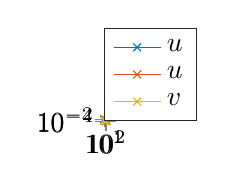
\begin{tikzpicture}

\begin{axis}[%
width=0.951\figwidth,
height=0.75\figwidth,
at={(0\figwidth,0\figwidth)},
scale only axis,
xmode=log,
xmin=4,
xmax=100,
xminorticks=true,
ymode=log,
ymin=1e-05,
ymax=0.1,
yminorticks=true,
axis background/.style={fill=white},
legend style={at={(0.03,0.03)}, anchor=south west, legend cell align=left, align=left, draw=white!15!black}
]
\addplot [color=mycolor1, mark=x, mark options={solid, mycolor1}]
  table[row sep=crcr]{%
4	0.0377253281\\
8	0.016292839\\
16	0.00647505826\\
32	0.00277859939\\
64	0.00131783073\\
};
\addlegendentry{$u$}

\addplot [color=mycolor2, mark=x, mark options={solid, mycolor2}]
  table[row sep=crcr]{%
4	0.00100309389\\
8	0.000409725552\\
16	0.000134946447\\
32	5.06672786e-05\\
64	2.29407924e-05\\
};
\addlegendentry{$u$}

\addplot [color=mycolor3, mark=x, mark options={solid, mycolor3}]
  table[row sep=crcr]{%
4	0.000631316968\\
8	0.000278812074\\
16	0.00010907144\\
32	4.76177485e-05\\
64	2.28652417e-05\\
};
\addlegendentry{$v$}

\addplot [color=white!70!black, forget plot]
  table[row sep=crcr]{%
4	0.00025\\
100	1e-05\\
};
\addplot [color=white!70!black, forget plot]
  table[row sep=crcr]
	\subfloat[Upwind, $Re = \num{e3}$]{
		\input{../img/l2error_test_navierstokes_sincos_hre}}\\
	\subfloat[Min-Mod, $Re = 1$]{
		% This file was created by matlab2tikz.
%
\definecolor{mycolor1}{rgb}{0.00000,0.44700,0.74100}%
\definecolor{mycolor2}{rgb}{0.85000,0.32500,0.09800}%
\definecolor{mycolor3}{rgb}{0.92900,0.69400,0.12500}%
%
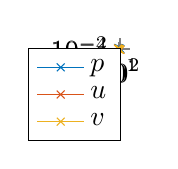
\begin{tikzpicture}

\begin{axis}[%
width=0.951\figwidth,
height=0.75\figwidth,
at={(0\figwidth,0\figwidth)},
scale only axis,
xmode=log,
xmin=4,
xmax=100,
xminorticks=true,
ymode=log,
ymin=1e-05,
ymax=0.1,
yminorticks=true,
axis background/.style={fill=white},
legend style={at={(0.97,0.97)}, anchor=north east, legend cell align=left, align=left}
]
\addplot [color=mycolor1, mark=x, mark options={solid, mycolor1}]
  table[row sep=crcr]{%
4	0.0201961443\\
8	0.00658170291\\
16	0.00181646151\\
32	0.000558641084\\
64	0.000188245776\\
};
\addlegendentry{$p$}

\addplot [color=mycolor2, mark=x, mark options={solid, mycolor2}]
  table[row sep=crcr]{%
4	0.00148598782\\
8	0.00053497283\\
16	0.000150385476\\
32	3.95894587e-05\\
64	1.01636468e-05\\
};
\addlegendentry{$u$}

\addplot [color=mycolor3, mark=x, mark options={solid, mycolor3}]
  table[row sep=crcr]{%
4	0.00119526142\\
8	0.00045470553\\
16	0.000138075359\\
32	3.80865907e-05\\
64	1.00057526e-05\\
};
\addlegendentry{$v$}

\addplot [color=white!70!black, forget plot]
  table[row sep=crcr]{%
4	0.00025\\
100	1e-05\\
};
\addplot [color=white!70!black, forget plot]
  table[row sep=crcr]
	\subfloat[Min-Mod, $Re = \num{e3}$]{
		\input{../img/l2error_test_navierstokes_sincos_mm_hre}}\\
	\subfloat[Van Leer, $Re = 1$]{
		% This file was created by matlab2tikz.
%
\definecolor{mycolor1}{rgb}{0.00000,0.44700,0.74100}%
\definecolor{mycolor2}{rgb}{0.85000,0.32500,0.09800}%
\definecolor{mycolor3}{rgb}{0.92900,0.69400,0.12500}%
%
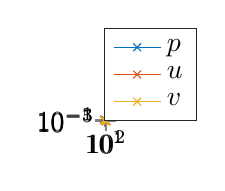
\begin{tikzpicture}

\begin{axis}[%
width=0.951\figwidth,
height=0.75\figwidth,
at={(0\figwidth,0\figwidth)},
scale only axis,
xmode=log,
xmin=4,
xmax=100,
xminorticks=true,
ymode=log,
ymin=8.63199669e-06,
ymax=0.1,
yminorticks=true,
axis background/.style={fill=white},
legend style={at={(0.03,0.03)}, anchor=south west, legend cell align=left, align=left, draw=white!15!black}
]
\addplot [color=mycolor1, mark=x, mark options={solid, mycolor1}]
  table[row sep=crcr]{%
4	0.017335487\\
8	0.0062618753\\
16	0.00193371119\\
32	0.000605597659\\
64	0.000196206927\\
};
\addlegendentry{$p$}

\addplot [color=mycolor2, mark=x, mark options={solid, mycolor2}]
  table[row sep=crcr]{%
4	0.00136409678\\
8	0.000476275877\\
16	0.000131606902\\
32	3.41242821e-05\\
64	8.66824542e-06\\
};
\addlegendentry{$u$}

\addplot [color=mycolor3, mark=x, mark options={solid, mycolor3}]
  table[row sep=crcr]{%
4	0.00114596769\\
8	0.000417513208\\
16	0.000122988533\\
32	3.32359157e-05\\
64	8.63199669e-06\\
};
\addlegendentry{$v$}

\addplot [color=white!70!black, forget plot]
  table[row sep=crcr]{%
4	0.00021579991725\\
100	8.63199669e-06\\
};
\addplot [color=white!70!black, forget plot]
  table[row sep=crcr]
	\subfloat[Van Leer, $Re = \num{e3}$]{
		% This file was created by matlab2tikz.
%
\definecolor{mycolor1}{rgb}{0.00000,0.44700,0.74100}%
\definecolor{mycolor2}{rgb}{0.85000,0.32500,0.09800}%
\definecolor{mycolor3}{rgb}{0.92900,0.69400,0.12500}%
%
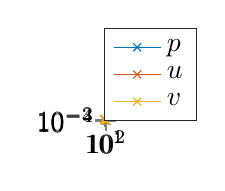
\begin{tikzpicture}

\begin{axis}[%
width=0.951\figwidth,
height=0.75\figwidth,
at={(0\figwidth,0\figwidth)},
scale only axis,
xmode=log,
xmin=4,
xmax=100,
xminorticks=true,
ymode=log,
ymin=0.0001,
ymax=0.01454297,
yminorticks=true,
axis background/.style={fill=white},
legend style={at={(0.03,0.03)}, anchor=south west, legend cell align=left, align=left, draw=white!15!black}
]
\addplot [color=mycolor1, mark=x, mark options={solid, mycolor1}]
  table[row sep=crcr]{%
4	0.01454297\\
8	0.00653869074\\
16	0.00224775854\\
32	0.0005196908\\
64	0.000249600967\\
};
\addlegendentry{$p$}

\addplot [color=mycolor2, mark=x, mark options={solid, mycolor2}]
  table[row sep=crcr]{%
4	0.0107200353\\
8	0.00466675248\\
16	0.00177426299\\
32	0.000645881865\\
64	0.000238530337\\
};
\addlegendentry{$u$}

\addplot [color=mycolor3, mark=x, mark options={solid, mycolor3}]
  table[row sep=crcr]{%
4	0.0112112271\\
8	0.00583504088\\
16	0.00263953931\\
32	0.00102531826\\
64	0.000347747564\\
};
\addlegendentry{$v$}

\addplot [color=white!70!black, forget plot]
  table[row sep=crcr]{%
4	0.0025\\
100	0.0001\\
};
\addplot [color=white!70!black, forget plot]
  table[row sep=crcr]
	\caption[$L^2$-errors for the Sin-Cos test]{$L^2$-errors for the Sin-Cos 
	test depending on the square root of the number of cells in the grid. 
	The grey lines are the reference lines for the first-order and second-order 
	convergence.}
	\label{fig:sin_err}
\end{figure}

\begin{table}
	\centering
	\[
	\begin{array}{c|ccc}
	\toprule
	& \text{Upwind} & \text{Min-Mod} & \text{Van Leer} \\ 
	\midrule
	p & 1.008 & 1.569 & 1.626\\
	v_x & 1.143 & 1.962 & 1.977\\
	v_y & 1.058 & 1.928 & 1.945\\
	\bottomrule
	\end{array}
	\]
	\caption[Convergence orders with $Re = 1$ for the Sin-Cos 
	test]{Convergence orders with $Re = 1$ for the Sin-Cos test. They are 
	computed considering the last two refinements of the grid.}
	\label{tab:sin_lre}
	\[
	\begin{array}{c|ccc}
	\toprule
	& \text{Upwind} & \text{Min-Mod} & \text{Van Leer} \\ 
	\midrule
	p & 1.148 & 1.659 & 1.058\\
	v_x & 1.071 & 1.441 & 1.437\\
	v_y & 1.068 & 1.533 & 1.560\\
	\bottomrule
	\end{array}
	\]
	\caption[Convergence orders with $Re = \num{e3}$ for the Sin-Cos 
	test]{Convergence orders with $Re = \num{e3}$ for the Sin-Cos test. 
	They are computed considering the last two refinements of the grid.}
	\label{tab:sin_hre}
\end{table}

We observe, as expected, a better behaviour of the TVD methods with respect to 
the upwind method. In Table~\ref{tab:sin_lre} we can see that at $Re=1$ the 
formers show a full second order convergence for the velocity, while for the 
rate is a bit lower; the latter instead shows a first for all the variables. At 
$Re=\num{e3}$ a slight decrease of the rates of the TVD methods occurs also for 
the velocities, but they remain higher then the ones of the upwind method. In 
Table~\ref{tab:sin_hre} we observe a convergence order of 1 for the pressure 
using the Van Leer flux limiter, but looking at Figure~\ref{fig:sin_err} we can 
see that the global trend indicates a convergence of higher order. Moreover it 
can be observed how, thanks to the faster convergence, on the same grid the 
absolute values of the errors reach smaller values using the TVD methods. 
Between the Min-Mod and Van Leer flux limiter it is hard to say which performs 
better, the results are very similar.

Analogous tests with other analytical solutions are reported in the 
Appendix~\ref{app:conv}. They show always a better convergence of the TVD 
methods with respect to the upwind method, but in some cases the convergence 
order of pressure and velocity behave differently.
%
\subsection{Time convergence}
We test the time convergence of the $L^\infty(0,T;L^2(\Omega))$ norm of the 
error of the solution of the Navier-Stokes equations, comparing the results 
obtained with the BE method \eqref{eq:be} and the BDF2 method \eqref{eq:bdf2}.\\
We consider the unsteady version of the 
equations~\eqref{eq:nssteadymass}--\eqref{eq:nssteadymom}:
\begin{align}
	\label{eq:nsunsteadymass} \nabla \cdot \mathbf{v} -h = 0&\\
	\label{eq:nsunsteadymom} \frac{\partial \mathbf{v}}{\partial t} +\nabla 
	\cdot (\mathbf{v} \mathbf{v}^\mathrm{T}) - 
	\nabla \cdot (\nu \nabla \mathbf{v}) + \frac{1}{\varrho}\nabla p  
	-\mathbf{f} = \mathbf{0}&
\end{align}
Again the gravity is neglected and two possible sources $h$ and $\mathbf{f}$ 
are taken into account, moreover all the quantities are considered to be 
non-dimensional.
%
\subsubsection{Unsteady Sin-Cos test}
Let us solve the equations~\eqref{eq:nsunsteadymass}--\eqref{eq:nsunsteadymom} 
over a two dimensional unit domain $\Omega=(0,1)^2$ and in the time interval 
$(0,T)$, with $T=1$. We use the following source terms:
\begin{align}
h &= 0,\\
\mathbf{f} &= 2\Big(\frac{\cos(2t)}{\varrho} + \nu \sin(2t)\Big)[- \cos(x) 
\sin(y), \; 
\cos(y) \sin(x)]^\mathrm{T},
\end{align}
so that, choosing $\varrho=1$, the analytical solution is given by
\begin{align}
\label{eq:uexunssin}	u_\text{ex}(x,y) &= -\cos(x)\sin(y)\sin(2t)\\
v_\text{ex}(x,y) &= \sin(x)\cos(y)\sin(2t)\\
\label{eq:pexunssin}	p_\text{ex}(x,y) &= 
-\frac{\cos(2x)+\sin(2y)}{4}\sin^2(2t),
\end{align}
so it is equal to \eqref{eq:uexsin}--\eqref{eq:pexsin}, used in the steady test 
for the space convergence, except for the modulation over time. We choose 
$\nu=0.1$, so that $Re=10$. Dirichlet boundary conditions for the velocity are 
applied on the whole boundary $\partial \Omega$ using the exact solution. 
Pressure is again fixed  at one point in order to match the exact solution 
\eqref{eq:pexunssin}.

The problem is solved seven times subdividing the time interval $(0,T)$ into 
uniform time-steps and each time time doubling their number, starting from a 
single time-step. Uniform grids of $\num{40x40}$ and $\num{80x80}$ cells are 
employed and as a differencing scheme the TVD method with the Van Leer flux 
limiter \eqref{eq:vl} is used. From Figure~\ref{fig:timeerr} we observe that, 
as expected, the BE method shows a first-order convergence, while the BDF2 
method is of second order. Moreover we notice that, with a grid of 
$\num{40x40}$ cells, in the last refinement the error with the BDF2 method does 
not decrease anymore. This happens because the spatial error becomes 
dominant, indeed refining the grid the convergence order is restored entirely 
for the pressure and almost for the velocity.
\begin{figure}
	\centering
	\subfloat{\input{../img/time_convergence_p_report}}
	\subfloat{% This file was created by matlab2tikz.
%
\definecolor{mycolor1}{rgb}{0.00000,0.44700,0.74100}%
\definecolor{mycolor2}{rgb}{0.85000,0.32500,0.09800}%
\definecolor{mycolor3}{rgb}{0.92900,0.69400,0.12500}%
%
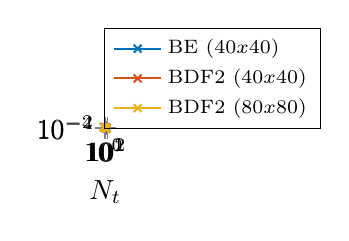
\begin{tikzpicture}

\begin{axis}[%
width=0.99\figwidth,
height=0.8\figwidth,
at={(0\figwidth,0\figwidth)},
scale only axis,
xmode=log,
xmin=1,
xmax=100,
xminorticks=true,
xlabel={$N_t$},
ymode=log,
ymin=1e-5,
ymax=1e-1,
yminorticks=true,
%ylabel style={font=\scriptsize},
%ylabel={$L^\infty$-error},
axis background/.style={fill=white},
legend style={at={(0.03,0.03)}, anchor=south west, legend cell align=left, fill=none,
align=left, font=\scriptsize}
]

\addplot [color=white!70!black, forget plot, line width=0.75pt]
  table[row sep=crcr]{%
1	0.1\\
100	0.001\\
};
\addplot [color=white!70!black, forget plot, line width=0.75pt]
  table[row sep=crcr]{%
1	0.1\\
100	0.00001\\
};
\addplot [color=mycolor1, mark=x, mark options={solid, mycolor1}, line width=0.75pt]
  table[row sep=crcr]{%
1	5.516e-2\\
2	3.043e-2\\
4	1.607e-2\\
8	8.216e-3\\
16	4.12e-3\\
32	2.03e-3\\
64	9.712e-4\\
};
\addlegendentry{BE ($\num{40x40}$)}

\addplot [color=mycolor2, mark=x, mark options={solid, mycolor2}, line width=0.75pt]
  table[row sep=crcr]{%
1	5.516e-2\\
2	1.645e-2\\
4	4.8e-3\\
8	1.21e-3\\
16	2.85e-4\\
32	1.3e-4\\
64	1.278e-4\\
};
\addlegendentry{BDF2 ($\num{40x40}$)}

\addplot [color=mycolor3, mark=x, mark options={solid, mycolor3}, line width=0.75pt]
  table[row sep=crcr]
	\caption[$L^\infty(0,T;L^2(\Omega))$-errors for the unsteady Sin-Cos 
	test]{$L^\infty(0,T;L^2(\Omega))$-errors for the unsteady Sin-Cos test 
	depending on the number of time-steps. On the left the errors for the 
	pressure, on the right the error for the magnitude of the velocity. The 
	grey lines are the reference lines for the first-order and second-order 
	convergence.}
	\label{fig:timeerr}
\end{figure}
%
\subsection{Rough channel test} \label{subsec:roughchannel}
We test the behaviour of the TVD methods compared to the upwind method solving 
the unsteady Navier-Stokes equations \eqref{eq:nsmass}--\eqref{eq:nsmom} in 
a two-dimensional channel with a rough (i.e. non-flat) lower boundary. The 
roughness consists of small evenly spaced cavities. Two different 
configurations are studied, one with shallow cavities, depicted in 
Figure~\ref{fig:roughdom}, and another with deeper cavities, depicted in 
Figure~\ref{fig:roughdomdeep}.

On the left boundary $\Gamma_\text{in}$ we set inflow boundary conditions 
\eqref{eq:inflow}, specifying an horizontal velocity
\begin{equation}
	\mathbf{v} = \mathbf{v}_\text{in} = [u_\text{in}, 0]^\mathrm{T}, \quad 
	u_\text{in} = \SI{1}{m/s}.
\end{equation}
On the lower and upper boundaries $\Gamma_w$ we set no-slip boundary conditions 
\eqref{eq:noslip}, while on the right boundary $\Gamma_\text{out}$ we set 
outflow boundary conditions \eqref{eq:outflow}, fixing the value of the pressure
\begin{equation}
	p = p_\text{ext} = \SI{1.1e5}{\pascal}.
\end{equation}
As initial conditions the velocity is set to zero everywhere, while the 
pressure is set to $p_\text{ext}$ everywhere. The density is 
$\varrho=\SI{1}{kg/m^3}$. The gravity contribution in \eqref{eq:nsmom} is 
neglected.
%
\subsubsection{Shallow cavities}
In the case of shallow cavities we use the domain in Figure~\ref{fig:roughdom} 
and we employ a uniform grid of $\num{95x50}$ cells. The problem is then solved 
over the time interval [$0,T$], with $T=\SI{10}{s}$; the initial time-step is 
$\Delta t=\SI{5e-3}{s}$, then it is adapted as explained in 
Section~\ref{sec:algeq}, allowing a maximum time-step of $\SI{0.1}{s}$. 
At first we set $\nu=\SI{5e-4}{m^2/s}$, so that $Re=\num{2e3}$. Since we do not 
have an analytical solution for this problem, we compute a \emph{reference 
solution} using the upwind method over a grid six times finer.

In Figure~\ref{fig:linecompshallow} we compare the profiles of the magnitude 
of the velocity along a section near the end of the channel, at 
$x=\SI{8.75}{m}$, i.e. at the middle of the last cavity.  The TVD solutions 
match the reference one, while the upwind solution shows a small shift, 
especially in the lower part of the channel, above the cavity. So, on a coarse 
grid, we obtain a solution that is the one we would obtain with the upwind 
method on a finer grid. In Table~\ref{tab:errshallow} we can see the $L^2$-norm 
of the errors between the coarse solutions and the reference one, computed 
along the section. As expected, the one related to the upwind method is at 
least one order of magnitude larger than the others. 
\begin{figure}
	\centering
	\includegraphics[width=\textwidth]{rough_domain2.pdf}
	\caption[Domain of the rough channel test with shallow cavities]{Domain of 
	the rough channel test with shallow cavities.}
	\label{fig:roughdom}
\end{figure}
\begin{figure}
	\centering
	\includegraphics[width=\textwidth]{rough_channel_vl_report.png}
	\caption[Magnitude of the velocity magnitude in the rough channel test with 
	shallow cavities]{Magnitude of the velocity magnitude $[\si{m/s}]$ in the 
	rough channel test with shallow cavities at $t=\SI{10}{s}$. $Re=\num{2e3}$, 
	Van Leer flux limiter.}
	\label{fig:roughchannelvl}
\end{figure}
\begin{figure}
	\centering
	% This file was created by matlab2tikz.
%
\definecolor{mycolor1}{rgb}{0.00000,0.44700,0.74100}%
\definecolor{mycolor2}{rgb}{0.85000,0.32500,0.09800}%
\definecolor{mycolor3}{rgb}{0.92900,0.69400,0.12500}%
\definecolor{mycolor4}{rgb}{0.49400,0.18400,0.55600}%
%
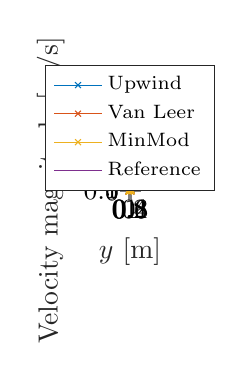
\begin{tikzpicture}

\begin{axis}[%
width=0.951\roughwidth,
height=0.75\roughheight,
at={(0\roughwidth,0\roughheight)},
scale only axis,
xmin=0,
xmax=1,
xlabel style={font=\color{white!15!black}},
xlabel={$y$ [m]},
ymin=0,
ymax=1.25,
ylabel style={font=\color{white!15!black}},
ylabel={Velocity magnitude [m/s]},
axis background/.style={fill=white},
legend style={at={(0.5,0.03)}, anchor=south, legend cell align=left, align=left, draw=white!15!black, font=\scriptsize}
]
\addplot [color=mycolor1, mark size=1.5pt, mark=x, mark options={solid, mycolor1}]
  table[row sep=crcr]{%
0	0\\
0.01	0.0293662\\
0.03	0.050586\\
0.05	0.0374104\\
0.07	0.00830816\\
0.09	0.0878588\\
0.11	0.203537\\
0.13	0.350154\\
0.15	0.504986\\
0.17	0.648407\\
0.19	0.773425\\
0.21	0.879108\\
0.23	0.965875\\
0.25	1.0347\\
0.27	1.08726\\
0.29	1.12581\\
0.31	1.15286\\
0.33	1.17097\\
0.35	1.18249\\
0.37	1.18938\\
0.39	1.19321\\
0.41	1.19513\\
0.43	1.19595\\
0.45	1.19618\\
0.47	1.19615\\
0.49	1.19606\\
0.51	1.19602\\
0.53	1.19608\\
0.55	1.19627\\
0.57	1.19661\\
0.59	1.19708\\
0.61	1.1977\\
0.63	1.19842\\
0.65	1.19918\\
0.67	1.19986\\
0.69	1.20024\\
0.71	1.19994\\
0.73	1.19831\\
0.75	1.19437\\
0.77	1.18669\\
0.79	1.17327\\
0.81	1.15154\\
0.83	1.11834\\
0.85	1.07018\\
0.87	1.00343\\
0.89	0.914856\\
0.91	0.802051\\
0.93	0.663892\\
0.95	0.500819\\
0.97	0.314904\\
0.99	0.109749\\
1	0\\
};
\addlegendentry{Upwind}

\addplot [color=mycolor2, mark size=1.5pt, mark=x, mark options={solid, mycolor2}]
  table[row sep=crcr]{%
0	0\\
0.01	0.0271697\\
0.03	0.0500789\\
0.05	0.0401093\\
0.07	0.00567534\\
0.09	0.0811925\\
0.11	0.199174\\
0.13	0.35443\\
0.15	0.52202\\
0.17	0.675188\\
0.19	0.804904\\
0.21	0.91139\\
0.23	0.996051\\
0.25	1.06075\\
0.27	1.10807\\
0.29	1.14103\\
0.31	1.16275\\
0.33	1.17616\\
0.35	1.18381\\
0.37	1.1877\\
0.39	1.18933\\
0.41	1.18969\\
0.43	1.18942\\
0.45	1.18894\\
0.47	1.18845\\
0.49	1.18804\\
0.51	1.18779\\
0.53	1.1877\\
0.55	1.18779\\
0.57	1.18804\\
0.59	1.18848\\
0.61	1.18909\\
0.63	1.18985\\
0.65	1.19073\\
0.67	1.19161\\
0.69	1.19229\\
0.71	1.1924\\
0.73	1.19132\\
0.75	1.18802\\
0.77	1.181\\
0.79	1.16815\\
0.81	1.14675\\
0.83	1.11359\\
0.85	1.06512\\
0.87	0.997859\\
0.89	0.908818\\
0.91	0.795828\\
0.93	0.657971\\
0.95	0.495791\\
0.97	0.311428\\
0.99	0.10845\\
1	0\\
};
\addlegendentry{Van Leer}

\addplot [color=mycolor3, mark size=1.5pt, mark=x, mark options={solid, mycolor3}]
  table[row sep=crcr]{%
0	0\\
0.01	0.0272093\\
0.03	0.0494723\\
0.05	0.0389859\\
0.07	0.00595636\\
0.09	0.0812851\\
0.11	0.198804\\
0.13	0.353914\\
0.15	0.5204\\
0.17	0.672249\\
0.19	0.801321\\
0.21	0.907555\\
0.23	0.992249\\
0.25	1.05727\\
0.27	1.10509\\
0.29	1.13867\\
0.31	1.16106\\
0.33	1.17513\\
0.35	1.18335\\
0.37	1.18771\\
0.39	1.18968\\
0.41	1.19029\\
0.43	1.19022\\
0.45	1.18987\\
0.47	1.18946\\
0.49	1.18912\\
0.51	1.18891\\
0.53	1.18887\\
0.55	1.18899\\
0.57	1.18928\\
0.59	1.18974\\
0.61	1.19035\\
0.63	1.19112\\
0.65	1.19197\\
0.67	1.19282\\
0.69	1.19344\\
0.71	1.19347\\
0.73	1.19226\\
0.75	1.18881\\
0.77	1.18163\\
0.79	1.16863\\
0.81	1.14714\\
0.83	1.11395\\
0.85	1.06554\\
0.87	0.998402\\
0.89	0.90948\\
0.91	0.796585\\
0.93	0.658719\\
0.95	0.496437\\
0.97	0.311872\\
0.99	0.108614\\
1	0\\
};
\addlegendentry{MinMod}

\addplot [color=mycolor4]
  table[row sep=crcr]{%
0	0\\
0.00166667	0.00492427\\
0.005	0.0138838\\
0.00833333	0.0219483\\
0.0116667	0.0291114\\
0.015	0.0353663\\
0.0183333	0.0407062\\
0.0216667	0.0451241\\
0.025	0.0486134\\
0.0283333	0.051167\\
0.0316667	0.0527786\\
0.035	0.0534416\\
0.0383333	0.0531503\\
0.0416667	0.0518985\\
0.045	0.0496806\\
0.0483333	0.0464911\\
0.0516667	0.042324\\
0.055	0.037174\\
0.0583333	0.0310358\\
0.0616667	0.0239061\\
0.065	0.0157914\\
0.0683333	0.00678684\\
0.0716667	0.00421506\\
0.075	0.0150977\\
0.0783333	0.0273447\\
0.0816667	0.0407005\\
0.085	0.0551595\\
0.0883333	0.0707355\\
0.0916667	0.0874415\\
0.095	0.105279\\
0.0983333	0.124233\\
0.101667	0.144291\\
0.105	0.165438\\
0.108333	0.187646\\
0.111667	0.210875\\
0.115	0.23507\\
0.118333	0.260158\\
0.121667	0.286047\\
0.125	0.312628\\
0.128333	0.33978\\
0.131667	0.367367\\
0.135	0.395245\\
0.138333	0.42327\\
0.141667	0.451298\\
0.145	0.479192\\
0.148333	0.506829\\
0.151667	0.534103\\
0.155	0.560921\\
0.158333	0.587212\\
0.161667	0.612919\\
0.165	0.638002\\
0.168333	0.662436\\
0.171667	0.686204\\
0.175	0.7093\\
0.178333	0.731723\\
0.181667	0.753476\\
0.185	0.774566\\
0.188333	0.795\\
0.191667	0.814784\\
0.195	0.833928\\
0.198333	0.852438\\
0.201667	0.870321\\
0.205	0.887585\\
0.208333	0.904234\\
0.211667	0.920276\\
0.215	0.935716\\
0.218333	0.950561\\
0.221667	0.964818\\
0.225	0.978495\\
0.228333	0.991598\\
0.231667	1.00414\\
0.235	1.01612\\
0.238333	1.02756\\
0.241667	1.03847\\
0.245	1.04885\\
0.248333	1.05871\\
0.251667	1.06808\\
0.255	1.07696\\
0.258333	1.08537\\
0.261667	1.09332\\
0.265	1.10082\\
0.268333	1.10789\\
0.271667	1.11454\\
0.275	1.12079\\
0.278333	1.12664\\
0.281667	1.13213\\
0.285	1.13725\\
0.288333	1.14203\\
0.291667	1.14648\\
0.295	1.15062\\
0.298333	1.15445\\
0.301667	1.158\\
0.305	1.16127\\
0.308333	1.16429\\
0.311667	1.16706\\
0.315	1.1696\\
0.318333	1.17192\\
0.321667	1.17404\\
0.325	1.17597\\
0.328333	1.17771\\
0.331667	1.17929\\
0.335	1.18071\\
0.338333	1.18198\\
0.341667	1.18311\\
0.345	1.18412\\
0.348333	1.18501\\
0.351667	1.18579\\
0.355	1.18647\\
0.358333	1.18706\\
0.361667	1.18757\\
0.365	1.188\\
0.368333	1.18836\\
0.371667	1.18866\\
0.375	1.1889\\
0.378333	1.18908\\
0.381667	1.18923\\
0.385	1.18933\\
0.388333	1.18939\\
0.391667	1.18942\\
0.395	1.18942\\
0.398333	1.1894\\
0.401667	1.18935\\
0.405	1.18928\\
0.408333	1.1892\\
0.411667	1.18911\\
0.415	1.189\\
0.418333	1.18888\\
0.421667	1.18876\\
0.425	1.18863\\
0.428333	1.18849\\
0.431667	1.18836\\
0.435	1.18822\\
0.438333	1.18808\\
0.441667	1.18794\\
0.445	1.1878\\
0.448333	1.18766\\
0.451667	1.18753\\
0.455	1.1874\\
0.458333	1.18727\\
0.461667	1.18715\\
0.465	1.18703\\
0.468333	1.18691\\
0.471667	1.1868\\
0.475	1.1867\\
0.478333	1.1866\\
0.481667	1.18651\\
0.485	1.18642\\
0.488333	1.18634\\
0.491667	1.18626\\
0.495	1.18619\\
0.498333	1.18613\\
0.501667	1.18607\\
0.505	1.18601\\
0.508333	1.18597\\
0.511667	1.18593\\
0.515	1.18589\\
0.518333	1.18586\\
0.521667	1.18584\\
0.525	1.18582\\
0.528333	1.18581\\
0.531667	1.1858\\
0.535	1.1858\\
0.538333	1.18581\\
0.541667	1.18582\\
0.545	1.18584\\
0.548333	1.18586\\
0.551667	1.18589\\
0.555	1.18593\\
0.558333	1.18597\\
0.561667	1.18602\\
0.565	1.18607\\
0.568333	1.18613\\
0.571667	1.18619\\
0.575	1.18626\\
0.578333	1.18634\\
0.581667	1.18642\\
0.585	1.18651\\
0.588333	1.1866\\
0.591667	1.1867\\
0.595	1.18681\\
0.598333	1.18692\\
0.601667	1.18703\\
0.605	1.18716\\
0.608333	1.18729\\
0.611667	1.18742\\
0.615	1.18756\\
0.618333	1.18771\\
0.621667	1.18786\\
0.625	1.18802\\
0.628333	1.18819\\
0.631667	1.18835\\
0.635	1.18853\\
0.638333	1.18871\\
0.641667	1.18889\\
0.645	1.18908\\
0.648333	1.18927\\
0.651667	1.18947\\
0.655	1.18967\\
0.658333	1.18987\\
0.661667	1.19007\\
0.665	1.19028\\
0.668333	1.19048\\
0.671667	1.19068\\
0.675	1.19089\\
0.678333	1.19108\\
0.681667	1.19128\\
0.685	1.19147\\
0.688333	1.19165\\
0.691667	1.19182\\
0.695	1.19197\\
0.698333	1.19212\\
0.701667	1.19224\\
0.705	1.19235\\
0.708333	1.19243\\
0.711667	1.19249\\
0.715	1.19252\\
0.718333	1.19251\\
0.721667	1.19246\\
0.725	1.19237\\
0.728333	1.19223\\
0.731667	1.19204\\
0.735	1.19178\\
0.738333	1.19146\\
0.741667	1.19107\\
0.745	1.19059\\
0.748333	1.19003\\
0.751667	1.18937\\
0.755	1.1886\\
0.758333	1.18772\\
0.761667	1.18671\\
0.765	1.18557\\
0.768333	1.18428\\
0.771667	1.18283\\
0.775	1.18122\\
0.778333	1.17942\\
0.781667	1.17743\\
0.785	1.17523\\
0.788333	1.17282\\
0.791667	1.17016\\
0.795	1.16726\\
0.798333	1.16409\\
0.801667	1.16064\\
0.805	1.15689\\
0.808333	1.15283\\
0.811667	1.14845\\
0.815	1.14372\\
0.818333	1.13862\\
0.821667	1.13315\\
0.825	1.12728\\
0.828333	1.12101\\
0.831667	1.1143\\
0.835	1.10714\\
0.838333	1.09953\\
0.841667	1.09143\\
0.845	1.08284\\
0.848333	1.07374\\
0.851667	1.06411\\
0.855	1.05394\\
0.858333	1.04321\\
0.861667	1.0319\\
0.865	1.02002\\
0.868333	1.00753\\
0.871667	0.994433\\
0.875	0.980713\\
0.878333	0.96636\\
0.881667	0.951363\\
0.885	0.935712\\
0.888333	0.919401\\
0.891667	0.90242\\
0.895	0.884765\\
0.898333	0.866428\\
0.901667	0.847407\\
0.905	0.827698\\
0.908333	0.807298\\
0.911667	0.786206\\
0.915	0.764423\\
0.918333	0.74195\\
0.921667	0.718789\\
0.925	0.694943\\
0.928333	0.670418\\
0.931667	0.645219\\
0.935	0.619353\\
0.938333	0.592828\\
0.941667	0.565653\\
0.945	0.537839\\
0.948333	0.509397\\
0.951667	0.48034\\
0.955	0.45068\\
0.958333	0.420433\\
0.961667	0.389615\\
0.965	0.358241\\
0.968333	0.326328\\
0.971667	0.293895\\
0.975	0.260961\\
0.978333	0.227546\\
0.981667	0.193668\\
0.985	0.15935\\
0.988333	0.124612\\
0.991667	0.0894758\\
0.995	0.0539638\\
0.998333	0.0180982\\
1	0\\
};
\addlegendentry{Reference}
\addplot [color=black, dashed]
  table[row sep=crcr]{%
0.1	0\\
0.1 1.25\\
};
\end{axis}
\end{tikzpicture}%
	\caption[Profile of the magnitude of the velocity in the rough channel with 
	shallow cavities at $Re=\num{2e3}$]{Profile of the magnitude of the 
	velocity $[\si{m/s}]$ in the rough channel with shallow cavities along the 
	section $x=\SI{8.75}{m}$, at $t=\SI{10}{s}$. $Re=\num{2e3}$. The region on 
	the left of the dashed line is inside the cavity.}
	\label{fig:linecompshallow}
\end{figure}
\begin{table}
	\centering
	\[
	\begin{array}{ccc}
	\toprule
	\text{Upwind} & \text{Van Leer} & \text{Van Alabada} \\
	\midrule
	\num{1.708e-4} & \num{9.556e-6} & \num{1.119e-5} \\
	\midrule
	\text{Min-Mod} & \text{Superbee} & \text{MC Limiter} \\
	\midrule
	\num{1.537e-5} &  \SI{8.335e-6} & \num{8.659e-6}\\
	\bottomrule
	\end{array}
	\]
	\caption[$L^2$-errors for the profile of the magnitude of the velocity in 
	the rough channel with shallow cavities at $Re=\num{2e3}$]{$L^2$-errors for 
	the profile of the magnitude of the velocity along a section at 
	$x=\SI{8.75}{m}$ and $t=\SI{10}{s}$ in the rough channel with shallow 
	cavities. $Re = \num{2e3}$.}
	\label{tab:errshallow}
\end{table}

We repeat the test choosing $\nu=\SI{1}{m^2/s}$, so that $Re=1$. In 
Figure~\ref{fig:linecompshallowlre} we see that all the solutions have the same 
profile, moreover in the cavity there is no recirculation. In 
Table~\ref{tab:errshallow_lre} the $L^2$-errors are reported; the upwind one is 
the bigger, but they are all very similar. So, in this situation of low $Re$, 
the benefit of using a high-resolution scheme is reduced.
\begin{figure}
	\centering
	% This file was created by matlab2tikz.
%
\definecolor{mycolor1}{rgb}{0.00000,0.44700,0.74100}%
\definecolor{mycolor2}{rgb}{0.85000,0.32500,0.09800}%
\definecolor{mycolor3}{rgb}{0.92900,0.69400,0.12500}%
\definecolor{mycolor4}{rgb}{0.49400,0.18400,0.55600}%
%
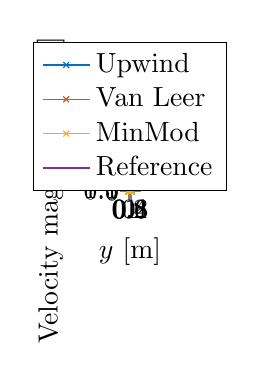
\begin{tikzpicture}

\begin{axis}[%
width=0.951\roughwidth,
height=0.75\roughheight,
at={(0\roughwidth,0\roughheight)},
scale only axis,
xmin=0,
xmax=1,
xlabel={$y$ [m]},
ymin=0,
ymax=1.5,
ylabel={Velocity magnitude [m/s]},
axis background/.style={fill=white},
legend style={at={(0.5,0.03)}, anchor=south, legend cell align=left, align=left}
]
\addplot [color=mycolor1, mark size=1.5pt, mark=x, mark options={solid, mycolor1}]
  table[row sep=crcr]{%
0	0\\
0.01	0.0254229\\
0.03	0.0771412\\
0.05	0.131431\\
0.07	0.189545\\
0.09	0.252263\\
0.11	0.319795\\
0.13	0.391594\\
0.15	0.466634\\
0.17	0.543711\\
0.19	0.621626\\
0.21	0.699267\\
0.23	0.775657\\
0.25	0.849957\\
0.27	0.921463\\
0.29	0.989594\\
0.31	1.05388\\
0.33	1.11392\\
0.35	1.16942\\
0.37	1.22012\\
0.39	1.26583\\
0.41	1.3064\\
0.43	1.34169\\
0.45	1.37161\\
0.47	1.39609\\
0.49	1.41506\\
0.51	1.42849\\
0.53	1.43632\\
0.55	1.43854\\
0.57	1.43512\\
0.59	1.42606\\
0.61	1.41134\\
0.63	1.39096\\
0.65	1.36491\\
0.67	1.3332\\
0.69	1.29582\\
0.71	1.25279\\
0.73	1.2041\\
0.75	1.14977\\
0.77	1.0898\\
0.79	1.02421\\
0.81	0.953007\\
0.83	0.876208\\
0.85	0.79383\\
0.87	0.705892\\
0.89	0.612418\\
0.91	0.513432\\
0.93	0.408963\\
0.95	0.299044\\
0.97	0.183712\\
0.99	0.063011\\
1	0\\
};
\addlegendentry{Upwind}

\addplot [color=mycolor2, mark size=1.5pt, mark=x, mark options={solid, mycolor2}]
  table[row sep=crcr]{%
0	0\\
0.01	0.0256098\\
0.03	0.0776368\\
0.05	0.132183\\
0.07	0.190504\\
0.09	0.253384\\
0.11	0.321031\\
0.13	0.392898\\
0.15	0.467961\\
0.17	0.54502\\
0.19	0.62289\\
0.21	0.700459\\
0.23	0.77675\\
0.25	0.850931\\
0.27	0.922307\\
0.29	0.990298\\
0.31	1.05443\\
0.33	1.11433\\
0.35	1.16969\\
0.37	1.22025\\
0.39	1.26584\\
0.41	1.30628\\
0.43	1.34146\\
0.45	1.37129\\
0.47	1.39566\\
0.49	1.41456\\
0.51	1.42791\\
0.53	1.43568\\
0.55	1.43786\\
0.57	1.4344\\
0.59	1.42531\\
0.61	1.41057\\
0.63	1.39018\\
0.65	1.36413\\
0.67	1.33242\\
0.69	1.29505\\
0.71	1.25203\\
0.73	1.20336\\
0.75	1.14905\\
0.77	1.08912\\
0.79	1.02356\\
0.81	0.952393\\
0.83	0.875636\\
0.85	0.793306\\
0.87	0.70542\\
0.89	0.612002\\
0.91	0.513077\\
0.93	0.408675\\
0.95	0.298828\\
0.97	0.183576\\
0.99	0.0629624\\
1	0\\
};
\addlegendentry{Van Leer}

\addplot [color=mycolor3, mark size=1.5pt, mark=x, mark options={solid, mycolor3}]
  table[row sep=crcr]{%
0	0\\
0.01	0.0255838\\
0.03	0.0775663\\
0.05	0.132074\\
0.07	0.190362\\
0.09	0.253217\\
0.11	0.320848\\
0.13	0.392711\\
0.15	0.467774\\
0.17	0.544841\\
0.19	0.622723\\
0.21	0.70031\\
0.23	0.776621\\
0.25	0.850825\\
0.27	0.92222\\
0.29	0.990231\\
0.31	1.05439\\
0.33	1.1143\\
0.35	1.16968\\
0.37	1.22026\\
0.39	1.26586\\
0.41	1.30632\\
0.43	1.34151\\
0.45	1.37134\\
0.47	1.39573\\
0.49	1.41463\\
0.51	1.42799\\
0.53	1.43577\\
0.55	1.43795\\
0.57	1.4345\\
0.59	1.42541\\
0.61	1.41067\\
0.63	1.39028\\
0.65	1.36422\\
0.67	1.33251\\
0.69	1.29514\\
0.71	1.25212\\
0.73	1.20345\\
0.75	1.14914\\
0.77	1.08919\\
0.79	1.02363\\
0.81	0.952462\\
0.83	0.8757\\
0.85	0.793364\\
0.87	0.705472\\
0.89	0.612048\\
0.91	0.513116\\
0.93	0.408706\\
0.95	0.298851\\
0.97	0.183591\\
0.99	0.0629675\\
1	0\\
};
\addlegendentry{MinMod}

\addplot [color=mycolor4]
  table[row sep=crcr]{%
0	0\\
0.00166667	0.00452198\\
0.005	0.0135298\\
0.00833333	0.0225133\\
0.0116667	0.0314839\\
0.015	0.0404525\\
0.0183333	0.0494296\\
0.0216667	0.0584251\\
0.025	0.0674484\\
0.0283333	0.0765086\\
0.0316667	0.0856141\\
0.035	0.0947727\\
0.0383333	0.103992\\
0.0416667	0.113279\\
0.045	0.122639\\
0.0483333	0.13208\\
0.0516667	0.141606\\
0.055	0.151223\\
0.0583333	0.160933\\
0.0616667	0.170742\\
0.065	0.180653\\
0.0683333	0.190669\\
0.0716667	0.200792\\
0.075	0.211024\\
0.0783333	0.221367\\
0.0816667	0.231823\\
0.085	0.242391\\
0.0883333	0.253073\\
0.0916667	0.263866\\
0.095	0.274774\\
0.0983333	0.285794\\
0.101667	0.296923\\
0.105	0.308161\\
0.108333	0.319508\\
0.111667	0.330959\\
0.115	0.342513\\
0.118333	0.354168\\
0.121667	0.365919\\
0.125	0.377765\\
0.128333	0.3897\\
0.131667	0.401723\\
0.135	0.413829\\
0.138333	0.426013\\
0.141667	0.438273\\
0.145	0.450603\\
0.148333	0.462999\\
0.151667	0.475457\\
0.155	0.487973\\
0.158333	0.50054\\
0.161667	0.513155\\
0.165	0.525812\\
0.168333	0.538508\\
0.171667	0.551237\\
0.175	0.563993\\
0.178333	0.576772\\
0.181667	0.58957\\
0.185	0.602381\\
0.188333	0.615201\\
0.191667	0.628024\\
0.195	0.640846\\
0.198333	0.653662\\
0.201667	0.666468\\
0.205	0.679258\\
0.208333	0.69203\\
0.211667	0.704776\\
0.215	0.717494\\
0.218333	0.730179\\
0.221667	0.742827\\
0.225	0.755434\\
0.228333	0.767995\\
0.231667	0.780507\\
0.235	0.792966\\
0.238333	0.805369\\
0.241667	0.81771\\
0.245	0.829988\\
0.248333	0.842198\\
0.251667	0.854338\\
0.255	0.866403\\
0.258333	0.878391\\
0.261667	0.890298\\
0.265	0.902123\\
0.268333	0.913861\\
0.271667	0.925509\\
0.275	0.937066\\
0.278333	0.948529\\
0.281667	0.959895\\
0.285	0.971162\\
0.288333	0.982327\\
0.291667	0.993388\\
0.295	1.00434\\
0.298333	1.01519\\
0.301667	1.02593\\
0.305	1.03655\\
0.308333	1.04706\\
0.311667	1.05746\\
0.315	1.06773\\
0.318333	1.07789\\
0.321667	1.08792\\
0.325	1.09784\\
0.328333	1.10763\\
0.331667	1.1173\\
0.335	1.12684\\
0.338333	1.13625\\
0.341667	1.14553\\
0.345	1.15468\\
0.348333	1.1637\\
0.351667	1.17258\\
0.355	1.18133\\
0.358333	1.18995\\
0.361667	1.19843\\
0.365	1.20677\\
0.368333	1.21498\\
0.371667	1.22305\\
0.375	1.23097\\
0.378333	1.23876\\
0.381667	1.24641\\
0.385	1.25391\\
0.388333	1.26127\\
0.391667	1.26849\\
0.395	1.27556\\
0.398333	1.28249\\
0.401667	1.28927\\
0.405	1.29591\\
0.408333	1.3024\\
0.411667	1.30875\\
0.415	1.31495\\
0.418333	1.321\\
0.421667	1.3269\\
0.425	1.33266\\
0.428333	1.33826\\
0.431667	1.34372\\
0.435	1.34902\\
0.438333	1.35417\\
0.441667	1.35918\\
0.445	1.36403\\
0.448333	1.36873\\
0.451667	1.37328\\
0.455	1.37768\\
0.458333	1.38191\\
0.461667	1.38601\\
0.465	1.38995\\
0.468333	1.39373\\
0.471667	1.39737\\
0.475	1.40085\\
0.478333	1.40417\\
0.481667	1.40735\\
0.485	1.41036\\
0.488333	1.41323\\
0.491667	1.41594\\
0.495	1.41849\\
0.498333	1.42089\\
0.501667	1.42313\\
0.505	1.42522\\
0.508333	1.42716\\
0.511667	1.42894\\
0.515	1.43056\\
0.518333	1.43202\\
0.521667	1.43334\\
0.525	1.43449\\
0.528333	1.43549\\
0.531667	1.43633\\
0.535	1.43702\\
0.538333	1.43755\\
0.541667	1.43792\\
0.545	1.43814\\
0.548333	1.4382\\
0.551667	1.4381\\
0.555	1.43785\\
0.558333	1.43744\\
0.561667	1.43687\\
0.565	1.43615\\
0.568333	1.43527\\
0.571667	1.43423\\
0.575	1.43304\\
0.578333	1.43168\\
0.581667	1.43017\\
0.585	1.4285\\
0.588333	1.42668\\
0.591667	1.4247\\
0.595	1.42256\\
0.598333	1.42026\\
0.601667	1.41781\\
0.605	1.4152\\
0.608333	1.41243\\
0.611667	1.40951\\
0.615	1.40642\\
0.618333	1.40319\\
0.621667	1.39979\\
0.625	1.39623\\
0.628333	1.39252\\
0.631667	1.38865\\
0.635	1.38462\\
0.638333	1.38044\\
0.641667	1.3761\\
0.645	1.3716\\
0.648333	1.36694\\
0.651667	1.36213\\
0.655	1.35715\\
0.658333	1.35202\\
0.661667	1.34674\\
0.665	1.34129\\
0.668333	1.33569\\
0.671667	1.32993\\
0.675	1.32402\\
0.678333	1.31794\\
0.681667	1.31171\\
0.685	1.30532\\
0.688333	1.29878\\
0.691667	1.29207\\
0.695	1.28521\\
0.698333	1.2782\\
0.701667	1.27102\\
0.705	1.26369\\
0.708333	1.2562\\
0.711667	1.24855\\
0.715	1.24075\\
0.718333	1.23279\\
0.721667	1.22467\\
0.725	1.2164\\
0.728333	1.20797\\
0.731667	1.19938\\
0.735	1.19064\\
0.738333	1.18174\\
0.741667	1.17268\\
0.745	1.16346\\
0.748333	1.15409\\
0.751667	1.14456\\
0.755	1.13488\\
0.758333	1.12504\\
0.761667	1.11504\\
0.765	1.10489\\
0.768333	1.09458\\
0.771667	1.08411\\
0.775	1.07349\\
0.778333	1.06271\\
0.781667	1.05177\\
0.785	1.04068\\
0.788333	1.02943\\
0.791667	1.01803\\
0.795	1.00647\\
0.798333	0.994758\\
0.801667	0.982888\\
0.805	0.970862\\
0.808333	0.958681\\
0.811667	0.946344\\
0.815	0.933851\\
0.818333	0.921203\\
0.821667	0.9084\\
0.825	0.895442\\
0.828333	0.882328\\
0.831667	0.86906\\
0.835	0.855636\\
0.838333	0.842058\\
0.841667	0.828325\\
0.845	0.814438\\
0.848333	0.800395\\
0.851667	0.786198\\
0.855	0.771847\\
0.858333	0.757342\\
0.861667	0.742682\\
0.865	0.727868\\
0.868333	0.712901\\
0.871667	0.697779\\
0.875	0.682504\\
0.878333	0.667075\\
0.881667	0.651492\\
0.885	0.635756\\
0.888333	0.619867\\
0.891667	0.603825\\
0.895	0.587629\\
0.898333	0.571281\\
0.901667	0.55478\\
0.905	0.538126\\
0.908333	0.521319\\
0.911667	0.504361\\
0.915	0.48725\\
0.918333	0.469987\\
0.921667	0.452572\\
0.925	0.435005\\
0.928333	0.417287\\
0.931667	0.399417\\
0.935	0.381396\\
0.938333	0.363224\\
0.941667	0.344901\\
0.945	0.326427\\
0.948333	0.307803\\
0.951667	0.289028\\
0.955	0.270103\\
0.958333	0.251028\\
0.961667	0.231803\\
0.965	0.212428\\
0.968333	0.192904\\
0.971667	0.173231\\
0.975	0.153409\\
0.978333	0.133438\\
0.981667	0.113319\\
0.985	0.0930514\\
0.988333	0.0726357\\
0.991667	0.0520722\\
0.995	0.0313611\\
0.998333	0.0105027\\
1	0\\
};
\addlegendentry{Reference}
\addplot [color=black, dashed]
  table[row sep=crcr]{%
0.1	0\\
0.1 1.5\\
};
\end{axis}
\end{tikzpicture}%
	\caption[Profile of the magnitude of the velocity in the rough channel with 
	shallow cavities at $Re=1$]{Profile of the magnitude of the velocity 
	$[\si{m/s}]$ in the rough channel with shallow cavities along the section 
	$x=\SI{8.75}{m}$, at $t=\SI{5}{s}$. $Re=1$. The region on the left of the 
	dashed line is inside the cavity.}
	\label{fig:linecompshallowlre}
\end{figure}
\begin{table}
	\centering
	\[
	\begin{array}{ccc}
	\toprule
	\text{Upwind} & \text{Van Leer} & \text{Van Alabada}\\
	\midrule
	\num{3.431e-6} & \num{2.917e-6} & \num{2.937e-6}\\
	\midrule
	\text{Min-Mod} & \text{Superbee} & \text{MC Limiter} \\ 
	\midrule
	\num{2.956e-6} & \num{2.899e-6} & \num{2.902e-6}\\
	\bottomrule
	\end{array}
	\]
	\caption[$L^2$-errors for the profile of the magnitude of the velocity in 
	the rough channel with shallow cavities at $Re=1$]{$L^2$-errors for the 
	profile of the magnitude of the velocity along a section at 
	$x=\SI{8.75}{m}$ and $t=\SI{5}{s}$ in the rough channel with shallow 
	cavities. $Re = 1$.}
	\label{tab:errshallow_lre}
\end{table}
%
\subsubsection{Deep cavities}
In the case of deep cavities we use the domain in Figure~\ref{fig:roughdomdeep} 
and we employ a uniform grid of $\num{95x70}$ cells. Again we solve until 
$T=\SI{10}{s}$, starting from an initial time-step of $\SI{e-3}{s}$. We set 
$\nu=\SI{5e-4}{m^2/s}$, so that $Re=\num{2.8e3}$. As before we compute a 
reference solution over a grid six times finer.

In Figure~\ref{fig:linecompdeep} we compare the profiles of the magnitude of 
the velocity along the section at $x=\SI{8.75}{m}$. Now the biggest differences 
are in the region inside the cavity, where the recirculation occurs. The upwind 
method, with its numerical diffusion, smooths the profile, while the TVD 
methods produce a more accurate result, even if they do not match exactly the 
reference solution. Indeed, looking at the $L^2$-errors reported in 
Table~\ref{tab:errdeep}, we see that the upwind has again the largest error, 
but the difference with the other schemes is reduced with respect to the 
previous case of shallow cavities.
\begin{figure}
	\centering
	\includegraphics[width=\textwidth]{rough_domain_highstep2.pdf}
	\caption[Domain of the rough channel test with deep cavities]{Domain of the 
	rough channel test with deep cavities.}
	\label{fig:roughdomdeep}
\end{figure}
\begin{figure}
	\centering
	% This file was created by matlab2tikz.
%
\definecolor{mycolor1}{rgb}{0.00000,0.44700,0.74100}%
\definecolor{mycolor2}{rgb}{0.85000,0.32500,0.09800}%
\definecolor{mycolor3}{rgb}{0.92900,0.69400,0.12500}%
\definecolor{mycolor4}{rgb}{0.49400,0.18400,0.55600}%
%
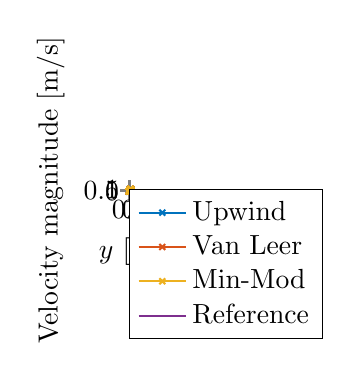
\begin{tikzpicture}

\begin{axis}[%
width=0.951\roughwidth,
height=0.75\roughheight,
at={(0\roughwidth,0\roughheight)},
scale only axis,
xmin=0,
xmax=1.4,
xlabel={$y$ [m]},
ymin=0,
ymax=1.25,
ylabel={Velocity magnitude [m/s]},
axis background/.style={fill=white},
legend style={at={(0.03,0.97)}, anchor=north west, legend cell align=left, align=left}
]

\addplot [color=mycolor1, mark size=1.5pt, mark=x, mark options={solid, mycolor1}, line width=0.75pt]
  table[row sep=crcr]{%
0	0\\
0.01	0.00885222\\
0.03	0.0227802\\
0.05	0.0327807\\
0.07	0.0393192\\
0.09	0.043122\\
0.11	0.0448784\\
0.13	0.0451341\\
0.15	0.0442874\\
0.17	0.0426208\\
0.19	0.0403378\\
0.21	0.037597\\
0.23	0.0345472\\
0.25	0.0313691\\
0.27	0.0283253\\
0.29	0.0258075\\
0.31	0.0243184\\
0.33	0.024277\\
0.35	0.0257093\\
0.37	0.0283224\\
0.39	0.0319839\\
0.41	0.0370173\\
0.43	0.044611\\
0.45	0.0576046\\
0.47	0.0818451\\
0.49	0.128213\\
0.51	0.214615\\
0.53	0.35431\\
0.55	0.509962\\
0.57	0.654372\\
0.59	0.77967\\
0.61	0.885193\\
0.63	0.971543\\
0.65	1.03985\\
0.67	1.0919\\
0.69	1.12994\\
0.71	1.15654\\
0.73	1.17426\\
0.75	1.18543\\
0.77	1.19201\\
0.79	1.19557\\
0.81	1.19723\\
0.83	1.1978\\
0.85	1.19779\\
0.87	1.19754\\
0.89	1.19723\\
0.91	1.19698\\
0.93	1.19685\\
0.95	1.19686\\
0.97	1.19703\\
0.99	1.19736\\
1.01	1.19783\\
1.03	1.19841\\
1.05	1.19906\\
1.07	1.19964\\
1.09	1.19992\\
1.11	1.19953\\
1.13	1.19783\\
1.15	1.19384\\
1.17	1.1861\\
1.19	1.17264\\
1.21	1.15086\\
1.23	1.11762\\
1.25	1.06938\\
1.27	1.00254\\
1.29	0.913831\\
1.31	0.800848\\
1.33	0.662508\\
1.35	0.499366\\
1.37	0.313659\\
1.39	0.109156\\
1.4	0\\
};
\addlegendentry{Upwind}

\addplot [color=mycolor2, mark size=1.5pt, mark=x, mark options={solid, mycolor2}, line width=0.75pt]
  table[row sep=crcr]{%
0	0\\
0.01	0.0122335\\
0.03	0.0324848\\
0.05	0.0480886\\
0.07	0.0588624\\
0.09	0.0654371\\
0.11	0.0686113\\
0.13	0.0688211\\
0.15	0.0669287\\
0.17	0.0627025\\
0.19	0.0563737\\
0.21	0.0484432\\
0.23	0.0398216\\
0.25	0.0319033\\
0.27	0.0265586\\
0.29	0.0256695\\
0.31	0.0288832\\
0.33	0.0340499\\
0.35	0.0396606\\
0.37	0.0450472\\
0.39	0.0499693\\
0.41	0.0545328\\
0.43	0.0595794\\
0.45	0.0677895\\
0.47	0.0859627\\
0.49	0.128135\\
0.51	0.214164\\
0.53	0.35562\\
0.55	0.519342\\
0.57	0.670222\\
0.59	0.798895\\
0.61	0.905422\\
0.63	0.991025\\
0.65	1.05726\\
0.67	1.10635\\
0.69	1.14101\\
0.71	1.16412\\
0.73	1.17855\\
0.75	1.18688\\
0.77	1.19113\\
0.79	1.19289\\
0.81	1.19325\\
0.83	1.1929\\
0.85	1.19227\\
0.87	1.19163\\
0.89	1.19106\\
0.91	1.19067\\
0.93	1.19044\\
0.95	1.19037\\
0.97	1.1905\\
0.99	1.19084\\
1.01	1.19135\\
1.03	1.19204\\
1.05	1.19284\\
1.07	1.19365\\
1.09	1.19427\\
1.11	1.19434\\
1.13	1.19322\\
1.15	1.1899\\
1.17	1.18285\\
1.19	1.16996\\
1.21	1.14851\\
1.23	1.11525\\
1.25	1.06662\\
1.27	0.999152\\
1.29	0.909811\\
1.31	0.796478\\
1.33	0.658286\\
1.35	0.495815\\
1.37	0.311267\\
1.39	0.108298\\
1.4	0\\
};
\addlegendentry{Van Leer}

\addplot [color=mycolor3, mark size=1.5pt, mark=x, mark options={solid, mycolor3}, line width=0.75pt]
  table[row sep=crcr]{%
0	0\\
0.01	0.0113419\\
0.03	0.0297822\\
0.05	0.0438459\\
0.07	0.0535293\\
0.09	0.0594514\\
0.11	0.0623285\\
0.13	0.0627341\\
0.15	0.0613312\\
0.17	0.0581295\\
0.19	0.0533229\\
0.21	0.0472654\\
0.23	0.040544\\
0.25	0.0340756\\
0.27	0.0291588\\
0.29	0.0272168\\
0.31	0.0284915\\
0.33	0.0317763\\
0.35	0.0359173\\
0.37	0.0402998\\
0.39	0.0446982\\
0.41	0.0493064\\
0.43	0.0551453\\
0.45	0.0648297\\
0.47	0.0848545\\
0.49	0.128268\\
0.51	0.214524\\
0.53	0.355773\\
0.55	0.518594\\
0.57	0.668691\\
0.59	0.796856\\
0.61	0.903066\\
0.63	0.988544\\
0.65	1.05485\\
0.67	1.10418\\
0.69	1.13918\\
0.71	1.16273\\
0.73	1.17764\\
0.75	1.1864\\
0.77	1.19104\\
0.79	1.19311\\
0.81	1.19369\\
0.83	1.19352\\
0.85	1.19301\\
0.87	1.19243\\
0.89	1.19193\\
0.91	1.19158\\
0.93	1.19138\\
0.95	1.19133\\
0.97	1.19148\\
0.99	1.19181\\
1.01	1.19232\\
1.03	1.19298\\
1.05	1.19375\\
1.07	1.19452\\
1.09	1.19508\\
1.11	1.19505\\
1.13	1.19379\\
1.15	1.1903\\
1.17	1.18309\\
1.19	1.17005\\
1.21	1.14852\\
1.23	1.11526\\
1.25	1.06673\\
1.27	0.999415\\
1.29	0.910241\\
1.31	0.797042\\
1.33	0.658892\\
1.35	0.496348\\
1.37	0.311635\\
1.39	0.108434\\
1.4	0\\
};
\addlegendentry{Min-Mod}

\addplot [color=mycolor4, line width=0.75pt]
  table[row sep=crcr]{%
0	0\\
0.00166667	0.00162965\\
0.005	0.00480799\\
0.00833333	0.00790634\\
0.0116667	0.0109252\\
0.015	0.013865\\
0.0183333	0.0167258\\
0.0216667	0.019508\\
0.025	0.022212\\
0.0283333	0.0248383\\
0.0316667	0.0273878\\
0.035	0.0298613\\
0.0383333	0.03226\\
0.0416667	0.0345853\\
0.045	0.0368385\\
0.0483333	0.0390211\\
0.0516667	0.0411348\\
0.055	0.0431809\\
0.0583333	0.045161\\
0.0616667	0.0470764\\
0.065	0.0489283\\
0.0683333	0.0507176\\
0.0716667	0.0524452\\
0.075	0.0541115\\
0.0783333	0.055717\\
0.0816667	0.0572619\\
0.085	0.0587457\\
0.0883333	0.0601683\\
0.0916667	0.0615291\\
0.095	0.0628271\\
0.0983333	0.0640617\\
0.101667	0.0652316\\
0.105	0.0663357\\
0.108333	0.0673728\\
0.111667	0.0683414\\
0.115	0.0692403\\
0.118333	0.070068\\
0.121667	0.0708231\\
0.125	0.0715044\\
0.128333	0.0721104\\
0.131667	0.0726401\\
0.135	0.0730923\\
0.138333	0.0734658\\
0.141667	0.0737601\\
0.145	0.0739741\\
0.148333	0.0741073\\
0.151667	0.0741594\\
0.155	0.0741298\\
0.158333	0.0740188\\
0.161667	0.0738262\\
0.165	0.0735523\\
0.168333	0.0731975\\
0.171667	0.0727624\\
0.175	0.0722478\\
0.178333	0.0716544\\
0.181667	0.0709837\\
0.185	0.0702367\\
0.188333	0.0694149\\
0.191667	0.0685199\\
0.195	0.0675533\\
0.198333	0.0665172\\
0.201667	0.0654135\\
0.205	0.0642444\\
0.208333	0.0630124\\
0.211667	0.0617197\\
0.215	0.0603692\\
0.218333	0.0589636\\
0.221667	0.0575058\\
0.225	0.055999\\
0.228333	0.0544466\\
0.231667	0.0528522\\
0.235	0.0512197\\
0.238333	0.0495534\\
0.241667	0.0478579\\
0.245	0.0461384\\
0.248333	0.0444006\\
0.251667	0.042651\\
0.255	0.0408971\\
0.258333	0.0391474\\
0.261667	0.0374118\\
0.265	0.0357016\\
0.268333	0.0340304\\
0.271667	0.032414\\
0.275	0.0308707\\
0.278333	0.0294217\\
0.281667	0.0280915\\
0.285	0.026907\\
0.288333	0.025897\\
0.291667	0.0250911\\
0.295	0.0245166\\
0.298333	0.0241958\\
0.301667	0.0241434\\
0.305	0.024363\\
0.308333	0.0248475\\
0.311667	0.0255795\\
0.315	0.0265348\\
0.318333	0.0276856\\
0.321667	0.0290029\\
0.325	0.0304586\\
0.328333	0.0320267\\
0.331667	0.0336841\\
0.335	0.0354105\\
0.338333	0.0371883\\
0.341667	0.0390024\\
0.345	0.0408399\\
0.348333	0.0426898\\
0.351667	0.0445425\\
0.355	0.04639\\
0.358333	0.048225\\
0.361667	0.0500416\\
0.365	0.0518343\\
0.368333	0.0535986\\
0.371667	0.0553303\\
0.375	0.0570259\\
0.378333	0.0586824\\
0.381667	0.060297\\
0.385	0.0618676\\
0.388333	0.0633923\\
0.391667	0.0648697\\
0.395	0.0662986\\
0.398333	0.0676785\\
0.401667	0.0690093\\
0.405	0.0702916\\
0.408333	0.0715265\\
0.411667	0.072716\\
0.415	0.0738628\\
0.418333	0.0749713\\
0.421667	0.076047\\
0.425	0.0770969\\
0.428333	0.0781306\\
0.431667	0.0791597\\
0.435	0.0801992\\
0.438333	0.0812674\\
0.441667	0.0823869\\
0.445	0.0835853\\
0.448333	0.084896\\
0.451667	0.0863585\\
0.455	0.08802\\
0.458333	0.0899355\\
0.461667	0.0921692\\
0.465	0.0947941\\
0.468333	0.0978929\\
0.471667	0.101558\\
0.475	0.105891\\
0.478333	0.111\\
0.481667	0.117001\\
0.485	0.124015\\
0.488333	0.13216\\
0.491667	0.141554\\
0.495	0.152307\\
0.498333	0.164518\\
0.501667	0.178267\\
0.505	0.193612\\
0.508333	0.210581\\
0.511667	0.229172\\
0.515	0.249346\\
0.518333	0.271026\\
0.521667	0.294097\\
0.525	0.318416\\
0.528333	0.3438\\
0.531667	0.370031\\
0.535	0.396864\\
0.538333	0.42408\\
0.541667	0.451482\\
0.545	0.478885\\
0.548333	0.506133\\
0.551667	0.533085\\
0.555	0.559629\\
0.558333	0.585678\\
0.561667	0.611162\\
0.565	0.636036\\
0.568333	0.660269\\
0.571667	0.683845\\
0.575	0.706758\\
0.578333	0.729008\\
0.581667	0.750601\\
0.585	0.771545\\
0.588333	0.79185\\
0.591667	0.811525\\
0.595	0.83058\\
0.598333	0.849024\\
0.601667	0.866863\\
0.605	0.884107\\
0.608333	0.900759\\
0.611667	0.916826\\
0.615	0.932313\\
0.618333	0.947225\\
0.621667	0.961569\\
0.625	0.975348\\
0.628333	0.988573\\
0.631667	1.00125\\
0.635	1.01338\\
0.638333	1.02498\\
0.641667	1.03605\\
0.645	1.04661\\
0.648333	1.05667\\
0.651667	1.06623\\
0.655	1.07531\\
0.658333	1.08392\\
0.661667	1.09207\\
0.665	1.09978\\
0.668333	1.10705\\
0.671667	1.11391\\
0.675	1.12035\\
0.678333	1.12641\\
0.681667	1.13209\\
0.685	1.1374\\
0.688333	1.14237\\
0.691667	1.147\\
0.695	1.15131\\
0.698333	1.15531\\
0.701667	1.15901\\
0.705	1.16244\\
0.708333	1.1656\\
0.711667	1.16851\\
0.715	1.17118\\
0.718333	1.17363\\
0.721667	1.17586\\
0.725	1.17789\\
0.728333	1.17974\\
0.731667	1.18141\\
0.735	1.18291\\
0.738333	1.18425\\
0.741667	1.18546\\
0.745	1.18653\\
0.748333	1.18747\\
0.751667	1.18831\\
0.755	1.18903\\
0.758333	1.18966\\
0.761667	1.1902\\
0.765	1.19066\\
0.768333	1.19104\\
0.771667	1.19135\\
0.775	1.19161\\
0.778333	1.19181\\
0.781667	1.19195\\
0.785	1.19206\\
0.788333	1.19212\\
0.791667	1.19214\\
0.795	1.19214\\
0.798333	1.19211\\
0.801667	1.19205\\
0.805	1.19197\\
0.808333	1.19188\\
0.811667	1.19177\\
0.815	1.19164\\
0.818333	1.19151\\
0.821667	1.19136\\
0.825	1.19121\\
0.828333	1.19106\\
0.831667	1.1909\\
0.835	1.19073\\
0.838333	1.19057\\
0.841667	1.19041\\
0.845	1.19025\\
0.848333	1.19009\\
0.851667	1.18993\\
0.855	1.18977\\
0.858333	1.18962\\
0.861667	1.18947\\
0.865	1.18933\\
0.868333	1.18919\\
0.871667	1.18906\\
0.875	1.18893\\
0.878333	1.18881\\
0.881667	1.18869\\
0.885	1.18858\\
0.888333	1.18847\\
0.891667	1.18838\\
0.895	1.18828\\
0.898333	1.1882\\
0.901667	1.18812\\
0.905	1.18804\\
0.908333	1.18797\\
0.911667	1.18791\\
0.915	1.18786\\
0.918333	1.18781\\
0.921667	1.18776\\
0.925	1.18773\\
0.928333	1.1877\\
0.931667	1.18767\\
0.935	1.18765\\
0.938333	1.18764\\
0.941667	1.18763\\
0.945	1.18763\\
0.948333	1.18764\\
0.951667	1.18765\\
0.955	1.18767\\
0.958333	1.18769\\
0.961667	1.18772\\
0.965	1.18776\\
0.968333	1.1878\\
0.971667	1.18785\\
0.975	1.1879\\
0.978333	1.18797\\
0.981667	1.18803\\
0.985	1.18811\\
0.988333	1.18818\\
0.991667	1.18827\\
0.995	1.18836\\
0.998333	1.18846\\
1.00167	1.18856\\
1.005	1.18867\\
1.00833	1.18879\\
1.01167	1.18891\\
1.015	1.18904\\
1.01833	1.18917\\
1.02167	1.18931\\
1.025	1.18946\\
1.02833	1.18961\\
1.03167	1.18977\\
1.035	1.18993\\
1.03833	1.1901\\
1.04167	1.19027\\
1.045	1.19045\\
1.04833	1.19063\\
1.05167	1.19081\\
1.055	1.191\\
1.05833	1.19119\\
1.06167	1.19139\\
1.065	1.19158\\
1.06833	1.19177\\
1.07167	1.19197\\
1.075	1.19216\\
1.07833	1.19235\\
1.08167	1.19253\\
1.085	1.19271\\
1.08833	1.19288\\
1.09167	1.19305\\
1.095	1.1932\\
1.09833	1.19333\\
1.10167	1.19345\\
1.105	1.19355\\
1.10833	1.19362\\
1.11167	1.19367\\
1.115	1.19369\\
1.11833	1.19368\\
1.12167	1.19363\\
1.125	1.19353\\
1.12833	1.19338\\
1.13167	1.19319\\
1.135	1.19293\\
1.13833	1.1926\\
1.14167	1.1922\\
1.145	1.19172\\
1.14833	1.19115\\
1.15167	1.19049\\
1.155	1.18971\\
1.15833	1.18883\\
1.16167	1.18782\\
1.165	1.18667\\
1.16833	1.18538\\
1.17167	1.18393\\
1.175	1.18231\\
1.17833	1.18051\\
1.18167	1.17852\\
1.185	1.17632\\
1.18833	1.17389\\
1.19167	1.17123\\
1.195	1.16832\\
1.19833	1.16515\\
1.20167	1.1617\\
1.205	1.15794\\
1.20833	1.15388\\
1.21167	1.14949\\
1.215	1.14475\\
1.21833	1.13965\\
1.22167	1.13417\\
1.225	1.12829\\
1.22833	1.12201\\
1.23167	1.11529\\
1.235	1.10812\\
1.23833	1.1005\\
1.24167	1.09239\\
1.245	1.08378\\
1.24833	1.07466\\
1.25167	1.06502\\
1.255	1.05483\\
1.25833	1.04408\\
1.26167	1.03276\\
1.265	1.02085\\
1.26833	1.00835\\
1.27167	0.995228\\
1.275	0.981485\\
1.27833	0.967108\\
1.28167	0.952085\\
1.285	0.936409\\
1.28833	0.92007\\
1.29167	0.903062\\
1.295	0.885377\\
1.29833	0.867011\\
1.30167	0.847959\\
1.305	0.828218\\
1.30833	0.807786\\
1.31167	0.786662\\
1.315	0.764846\\
1.31833	0.742339\\
1.32167	0.719144\\
1.325	0.695264\\
1.32833	0.670704\\
1.33167	0.645471\\
1.335	0.619571\\
1.33833	0.593012\\
1.34167	0.565805\\
1.345	0.537959\\
1.34833	0.509487\\
1.35167	0.480401\\
1.355	0.450714\\
1.35833	0.420443\\
1.36167	0.389601\\
1.365	0.358207\\
1.36833	0.326277\\
1.37167	0.29383\\
1.375	0.260885\\
1.37833	0.227463\\
1.38167	0.193583\\
1.385	0.159268\\
1.38833	0.124538\\
1.39167	0.0894149\\
1.395	0.0539223\\
1.39833	0.0180823\\
1.4	0\\
};
\addlegendentry{Reference}
\addplot [color=black, dashed, line width=0.75pt]
  table[row sep=crcr]{%
0.5	0\\
0.5 1.25\\
};
\end{axis}
\end{tikzpicture}%
	\caption[Profile of the magnitude of the velocity in the rough channel with 
	deep cavities at $Re=\num{2.8e3}$]{Profile of the magnitude of the velocity 
		$[\si{m/s}]$ in the rough channel with deep cavities along the section 
		$x=\SI{8.75}{m}$, at $t=\SI{10}{s}$. $Re=\num{2.8e3}$. The region on 
		the 
		left of the dashed line is inside the cavity.}
	\label{fig:linecompdeep}
\end{figure}
\begin{table}
	\centering
	\[
	\begin{array}{ccc}
	\toprule
	\text{Upwind} & \text{Van Leer} & \text{Van Alabada}\\
	\midrule
	\num{3.180e-4} & \num{5.862e-5} & \num{6.900e-5}\\
	\midrule
	\text{Min-Mod} & \text{Superbee} & \text{MC Limiter} \\
	\midrule
	\num{8.579e-5} & \num{7.883e-5} & \num{5.584e-5}\\
	\bottomrule
	\end{array}
	\]
	\caption[$L^2$-errors for the profile of the magnitude of the velocity in 
	the rough channel with deep cavities]{$L^2$-errors for the profile of the 
	magnitude of the velocity along a section at $x=\SI{8.75}{m}$ and 
	$t=\SI{10}{s}$ in the rough channel with deep cavities. $Re = \num{2.8e3}$.}
	\label{tab:errdeep}
\end{table}
%
\section{RANS test}
\subsection{Backward facing step}
The backward facing step is a widely-used test configuration, in which a turbulent flow in a channel incurs separation because of a sudden enlargement in the flow domain. As we can see in Figure~\ref{fig:bfsarrows}, there is a big recirculation after the step, a corner eddy and a very small eddy precisely at the corner. We want to use this test in order to compare the results that we obtain using the TVD method, with the Van Leer flux limiter \eqref{eq:vl}, and the $k\text{-}\omega$ turbulence model with the numerical results from \cite{web:nasa}, computed using the NASA CFL3D code, and the experimental results from \cite{bfs:driver}.

In the domain $\Omega$, depicted in Figure~\ref{fig:bfsdomain}, with a step height $H=\SI{1}{m}$, we solve the RANS equations \eqref{eq:ransmass}-\eqref{eq:ransmom}-\eqref{eq:komegak}-\eqref{eq:komegaomega}, imposing inflow boundary conditions on the left boundary $\Gamma_\text{in}$
\begin{equation}
	\mathbf{v} = \mathbf{v}_\text{in} = [u_\text{in}, 0]^\mathrm{T}, \quad u_\text{in} = \SI{44.2}{m/s},
\end{equation} no-slip boundary conditions on the lower and upper boundaries $\Gamma_w$ and outflow boundary conditions on the right boundary $\Gamma_\text{out}$, fixing the value of pressure
\begin{equation}
	p = p_\text{ext} = \SI{1.1e5}{\pascal}.
\end{equation}
\begin{figure}
	\centering
%	\includegraphics[width=\textwidth]{bfs_domain.pdf}
	\includegraphics[width=\textwidth]{bfs_domain_axis.pdf}
	\caption[Domain of the backward facing step test]{Domain $\Omega$ of the backward facing step test. For convenience, we set the position $x=0$ at the step and the position $y=0$ at the bottom of the channel.}
	\label{fig:bfsdomain}
\end{figure}
The density is $\varrho = \SI{1}{kg/m^3}$ and the viscosity is $\nu=\SI{1.228e-3}{m^2/s}$, so that, in order to match \cite{web:nasa}, the Reynolds number based on the step height results
\begin{equation}
	Re_H = \frac{u_\text{in}H}{\nu} \simeq \num{3.6e4}.
\end{equation}

The domain sizes are chosen according to \cite{web:nasa}, with the only exception of the channel length before the step. Indeed, in \cite{web:nasa}, a small portion of the horizontal boundary near $\Gamma_\text{in}$ uses symmetry boundary conditions, but we simplify the model employing no-slip boundary conditions on the whole horizontal boundaries. As a consequence, we shorten the channel length in order to match as good as possible the profile of the $u$ component of the velocity along the section at the position $x/H=-4$, with a boundary layer thickness of approximately $1.5H$ (see Figure~\ref{fig:bfscomp}).

According to \cite{web:nasa}, CFL3D is a code for compressible fluids, but it was used at ``essentially incompressible'' conditions, such that the influence of compressibility should be very small. Moreover it is reported that, running unsteady simulations, the solution settles down and becomes reasonably steady (quasi-steady); in \cite{bfs:cfl3d} it is explained that implicit methods for ad advancement in time are used.

Thus we employ the BDF2 method for non-constant time-steps \eqref{eq:bdf2gen}, starting from $\Delta t = \SI{e-5}{s}$ and simulating until $T_\text{end} = \SI{30}{s}$. It can be observed that after approximately $t=\SI{20}{s}$ the solution stabilizes at a steady state. As initial conditions we set
\begin{equation}
p=p_\text{ext} \quad \forall \mathbf{x} \in \Omega, \quad \mathbf{v} = [u_\text{init},0]^\mathrm{T} \quad u_\text{init} = \begin{cases}
u_\text{in} \quad&\text{if $x\leq 0$}\\
\frac{8}{9}u_\text{in} \quad&\text{if $x>0$}
\end{cases}
\end{equation}
The factor $8/9$ ensures that the discharge at $\Gamma_\text{in}$ and at $\Gamma_\text{out}$ is the same. For $k$ and $\omega$ we set in the whole domain the values estimated with \eqref{eq:koic}.

According to \cite{web:nasa}, a key indicator for the reliability of a simulation is the prediction of the \emph{reattachment length} $l_\text{rea}$, i.e. the distance after the step at which the recirculation finishes and thus the $u$ component of the velocity at the bottom of the channel becomes positive. We analyse this length computing the \emph{friction coefficient} $C_f$, that is a non-dimensional form of the stress at the wall, and it is defined by:
\begin{equation}
C_f = \frac{\tau_w}{\frac{1}{2}\varrho U_\text{ref}^2}, \quad \tau_w = \mu \frac{\partial u}{\partial y} \Big|_{y=0}.
\end{equation}
$U_\text{ref}$ is the $u$ component of the velocity at $x/H=-4$ and it is the characteristic value that we use to produce non-dimensional results. In our case when $C_f<0$ the flow is recirculating, then at $x=l_{rea}$ it becomes positive. The numerical results from \cite{web:nasa} predict $l_\text{rea}/H \simeq 6.8$, while the experimental results from \cite{bfs:driver} predict $l_\text{rea}/H = 6.26 \pm 0.10$, as it can be seen in Figure~\ref{fig:bfscf}.

Performing a sensitivity analysis in order to choose a suitable grid, we observed that
\begin{itemize}
	\item with a coarse mesh the reattachment length decreases, in particular a refinement of the smallest cell in the $y$-direction in effective.
	\item too stretched cells increase the number of Newton iteration needed to get the convergence of the problem.
	\item the cells in portion of the channel after the step can be coarsened in the $x$-direction without a great influence on the solution.
	\item too refined cells in the $y$-direction in the area with the recirculation do not improve in a relevant way the solution.
\end{itemize}
So, for the following analysis, we choose a grid made of $\num{119x70}$ cells, employing gradings up to 1.25 in order to have small cells near the walls.

\begin{figure}[p] %mettere in paraview frecce 2d
	\centering
	\includegraphics[width=\textwidth]{bfs_glimphs2.png}
	\caption[Velocity field after the backward facing step]{Velocity field $[\si{m/s}]$ after the backward facing step. $Re_H=\num{3.6e4}$. The arrows are not scaled.}
	\label{fig:bfsarrows}
\end{figure}
\begin{figure}[p]
	\centering
	\input{../img/bfs_fin_cf_report}
	\caption[Friction coefficient in the backward facing step test]{Friction coefficient at the bottom of the channel after the backward facing step. The reattachment length is the distance at which it becomes positive after its global minimum.}
	\label{fig:bfscf}
\end{figure}

Fo what concerns the reattachment length, we obtain a good agreement with the CFL3D code, indeed, looking at Figure~\ref{fig:bfscf}, with the Van Leer flux limiter we predict $l_\text{rea} /H \simeq 6.67$. Moreover, in the whole recirculating region, the pattern is very similar, also compared the experimental data from \cite{bfs:driver}. Using the first order upwind methods, instead, it is $l_\text{rea} /H \simeq 6.02$, so approximately a 10\% underestimation occurs. From the profile is seems that the whole recirculation is slightly smaller. Looking at the value near the end of the channel instead both the Van Leer and the upwind show a lower value with respect to the CFL3D code. Comparing in Figure~\ref{fig:bfscomp} the profiles of the $u$ component of the velocity along some section downstream with respect to the step, we obtain in a similarly a good agreement between the Van Leer result and the one from the CFL3D code, while the result from the upwind method presents a small shift, in particular in the cases $x/H=4$ and $x/H=10$. Along the section at $x/H=1$ the velocity at the wall is positive for the Van Leer and the CFL3D, since we are in correspondence of the corner eddy. For the upwind method, instead, the velocity is negative, as we are already in the bigger eddy because the whole pattern is anticipated.
\begin{figure}[ht]
	\centering
	\subfloat[$x/H=-4$]{\input{../img/bfs_fin_vel0_report}}
	\subfloat[$x/H=1$]{% This file was created by matlab2tikz.
%
\definecolor{mycolor4}{rgb}{0.00000,0.44700,0.74100}%
\definecolor{mycolor3}{rgb}{0.85000,0.32500,0.09800}%
\definecolor{mycolor2}{rgb}{0.92900,0.69400,0.12500}%
\definecolor{mycolor1}{rgb}{0.49400,0.18400,0.55600}%
%
\begin{tikzpicture}

\begin{axis}[%
width=0.958\bfshalfwidth,
height=0.75\bfsheight,
at={(0\bfshalfwidth,0\bfsheight)},
scale only axis,
xmin=-0.2,
xmax=1.2,
xlabel={$u/U_\text{ref}$},
ymin=0,
ymax=2,
ytick distance=1,
ylabel style={rotate=-90},
ylabel={$\dfrac{y}{H}$},
axis background/.style={fill=white},
legend style={at={(0.03,0.97)}, anchor=north west, legend cell align=left, align=left, font=\footnotesize, fill=none}
]
\addplot [color=mycolor1, line width=0.75pt]
  table[row sep=crcr]{%
0	0\\
0.0001201796986	0.0001500749349\\
0.0002449547756	0.0003087310179\\
0.0003762734123	0.0004765522899\\
0.0005145065952	0.0006541581242\\
0.0006600376801	0.0008422057144\\
0.000813261373	0.001041392214\\
0.0009745839634	0.00125245715\\
0.001144421869	0.001476185862\\
0.001323200529	0.001713411068\\
0.001511353068	0.001965016825\\
0.001709318836	0.002231941791\\
0.001917539747	0.002515181201\\
0.00213646004	0.002815792104\\
0.002366520697	0.003134895815\\
0.002608157694	0.003473682096\\
0.002861796878	0.003833413823\\
0.003127847333	0.004215430468\\
0.003406698816	0.004621152766\\
0.003698710818	0.005052087829\\
0.004004209302	0.005509833805\\
0.0043234732	0.005996085238\\
0.004656726494	0.006512639113\\
0.005004127044	0.007061398588\\
0.005365749821	0.007644380908\\
0.005741576198	0.008263722993\\
0.006131470203	0.008921687491\\
0.00653516734	0.009620669298\\
0.006952241063	0.0103632044\\
0.007382081822	0.01115197316\\
0.007823864929	0.0119898105\\
0.008276509121	0.0128797153\\
0.008738632314	0.01382485218\\
0.00920849666	0.0148285646\\
0.009683942422	0.01589438133\\
0.01016229764	0.01702602394\\
0.01064029057	0.0182274133\\
0.01111392584	0.01950268447\\
0.01157834847	0.02085618302\\
0.01202771906	0.02229248732\\
0.01245508343	0.023816403\\
0.01285232976	0.02543297783\\
0.01321025286	0.02714750916\\
0.01351886801	0.02896554396\\
0.013767967	0.03089288995\\
0.01394800935	0.03293561935\\
0.01405109838	0.03510007635\\
0.01407186221	0.03739286959\\
0.01400783751	0.03982088342\\
0.01385922916	0.04239127785\\
0.01362809725	0.04511147365\\
0.01331724878	0.04798916727\\
0.01292915177	0.05103230849\\
0.01246509328	0.05424910039\\
0.01192465518	0.0576479882\\
0.01130547561	0.0612376295\\
0.01060321368	0.06502689421\\
0.009811639786	0.06902483106\\
0.008922834881	0.07324063778\\
0.007927447557	0.07768364996\\
0.006814987864	0.08236327022\\
0.005573913921	0.08728893846\\
0.004191290587	0.09247011691\\
0.00265187677	0.09791619331\\
0.0009385751327	0.1036364213\\
-0.000963122875	0.1096399054\\
-0.003060560208	0.1159354597\\
-0.005352776032	0.1225315928\\
-0.00783053413	0.1294363886\\
-0.01047685929	0.1366574168\\
-0.01326751336	0.1442016512\\
-0.01617241837	0.1520753801\\
-0.01915765554	0.1602840871\\
-0.02218494006	0.1688323319\\
-0.02521179989	0.1777237058\\
-0.02819362469	0.1869606376\\
-0.03108495846	0.1965443641\\
-0.0338409096	0.2064747959\\
-0.03641942516	0.2167504281\\
-0.03878329694	0.2273682207\\
-0.04090159386	0.2383235991\\
-0.04275062308	0.249610275\\
-0.04431445152	0.2612203062\\
-0.04558489099	0.2731439471\\
-0.04656100646	0.2853696942\\
-0.04724829271	0.2978843451\\
-0.04765757173	0.3106728196\\
-0.0478037782	0.323718369\\
-0.04770476744	0.3370026648\\
-0.04738013446	0.3505057096\\
-0.04685027897	0.3642061055\\
-0.04613560811	0.3780810535\\
-0.04525596648	0.3921067119\\
-0.04423021153	0.4062580764\\
-0.04307601228	0.4205094278\\
-0.04180970788	0.4348344207\\
-0.04044631869	0.4492062032\\
-0.0389995873	0.4635978639\\
-0.03748202324	0.4779824615\\
-0.0359050557	0.492333293\\
-0.03427907825	0.5066241622\\
-0.03261359036	0.520829618\\
-0.03091723472	0.5349249244\\
-0.02919791639	0.5488865972\\
-0.02746286616	0.5626922846\\
-0.02571871504	0.5763211846\\
-0.02397154085	0.5897538066\\
-0.02222687751	0.6029724479\\
-0.02048963681	0.615961194\\
-0.01876389422	0.6287056804\\
-0.01705254801	0.6411936283\\
-0.01535683684	0.6534144878\\
-0.01367580146	0.6653595567\\
-0.01200577244	0.6770219207\\
-0.01033997722	0.6883966327\\
-0.008668510243	0.6994803548\\
-0.006978513673	0.7102713585\\
-0.005254388321	0.7207696438\\
-0.003478127997	0.7309766412\\
-0.001629842911	0.7408953309\\
0.0003117911983	0.7505297661\\
0.002369261347	0.7598854303\\
0.004565290641	0.7689688206\\
0.0069238469	0.7777875066\\
0.009470882826	0.7863498926\\
0.01223075204	0.794665277\\
0.0152295148	0.8027436137\\
0.01849941164	0.8105954528\\
0.02206458524	0.8182319403\\
0.02592881024	0.8256042004\\
0.0300907474	0.8326897025\\
0.03455769271	0.8394981027\\
0.03933769464	0.8460389972\\
0.04443381354	0.8523222208\\
0.04984596372	0.8583575487\\
0.0555716306	0.8641546965\\
0.06160631776	0.8697232008\\
0.06794383377	0.8750725389\\
0.07457635552	0.8802121878\\
0.08149473369	0.8851511478\\
0.08868864924	0.8898984194\\
0.09614694118	0.8944627047\\
0.1038577408	0.8988524675\\
0.1118080467	0.9030758739\\
0.1199838817	0.9071409106\\
0.1283706129	0.9110552073\\
0.1369528472	0.9148262739\\
0.1457143724	0.918461144\\
0.154637903	0.9219666123\\
0.1637056172	0.9253494143\\
0.1728995144	0.9286156893\\
0.1822014153	0.9317715764\\
0.1915930361	0.9348228574\\
0.2010559142	0.9377749562\\
0.2105716169	0.9406331778\\
0.2201218307	0.9434025884\\
0.2296884507	0.9460878968\\
0.2392538488	0.9486937523\\
0.2488009483	0.9512243867\\
0.2583136857	0.953684032\\
0.2677771151	0.9560765624\\
0.277177304	0.9584057331\\
0.286501348	0.9606750607\\
0.295737803	0.9628879428\\
0.3048765957	0.9650474787\\
0.3139089346	0.9671568274\\
0.3228273988	0.9692187309\\
0.3316257298	0.9712360501\\
0.3402987123	0.9732112885\\
0.3488423824	0.9751468897\\
0.3572541475	0.9770451784\\
0.3655327559	0.9789084196\\
0.3736785948	0.9807386398\\
0.3816936612	0.982537806\\
0.3895806074	0.9843078852\\
0.3973421156	0.9860506058\\
0.4049801826	0.9877676368\\
0.4124955237	0.9894605279\\
0.4198876917	0.9911309481\\
0.4271561205	0.9927802086\\
0.4343010783	0.9944097996\\
0.4413248301	0.9960208535\\
0.4482325017	0.9976147413\\
0.4550318718	0.9991925955\\
0.4617332518	1.000755548\\
0.4683483839	1.002304673\\
0.4748881757	1.003840923\\
0.4813614488	1.005365252\\
0.4877739847	1.006878734\\
0.4941294789	1.008381963\\
0.5004304647	1.009876132\\
0.506678462	1.011361718\\
0.5128827095	1.012839675\\
0.5190678239	1.014318705\\
0.5252566934	1.015807629\\
0.5314542055	1.017307401\\
0.537656188	1.018818736\\
0.5438578725	1.02034235\\
0.5500535369	1.021879435\\
0.5562369227	1.023430705\\
0.5624008775	1.024997234\\
0.5685377121	1.026580215\\
0.5746390224	1.02818048\\
0.5806956887	1.029799461\\
0.5866978765	1.031438231\\
0.5926355124	1.033098221\\
0.5984978676	1.034780741\\
0.6042742729	1.036487222\\
0.6099542379	1.038219213\\
0.6155272126	1.039978385\\
0.6209841967	1.041766405\\
0.6263165474	1.043585062\\
0.6315172315	1.045436382\\
0.6365810037	1.047322392\\
0.6415042877	1.049245119\\
0.6462858915	1.051206946\\
0.6509258747	1.053210378\\
0.6554266214	1.055257797\\
0.6597916484	1.057352066\\
0.6640262008	1.059496045\\
0.6681365371	1.061692715\\
0.6721298695	1.063945413\\
0.6760143042	1.066257596\\
0.6797982454	1.068632841\\
0.6834904552	1.071074963\\
0.6870999336	1.073588252\\
0.6906355023	1.076176882\\
0.6941058636	1.078845739\\
0.6975193024	1.081599474\\
0.7008841038	1.08444345\\
0.7042078376	1.08738327\\
0.707497716	1.090424657\\
0.7107604742	1.093573928\\
0.7140023708	1.096837759\\
0.7172290087	1.100223184\\
0.7204455137	1.103737593\\
0.723656714	1.107388973\\
0.7268668413	1.111185789\\
0.7300795913	1.115136862\\
0.7332985401	1.119251847\\
0.7365266085	1.123540759\\
0.739766717	1.128014207\\
0.743021071	1.132683516\\
0.7462921739	1.137560844\\
0.7495819926	1.142658949\\
0.7528924346	1.14799118\\
0.7562254667	1.153571963\\
0.7595828772	1.159416676\\
0.7629670501	1.165541291\\
0.7663809061	1.171962857\\
0.7698261142	1.178699493\\
0.7733042836	1.185770392\\
0.7768170238	1.19319582\\
0.7803665996	1.200997233\\
0.7839553952	1.209197283\\
0.7875868678	1.217820168\\
0.791264832	1.226891041\\
0.794998765	1.236445308\\
0.7988060117	1.246588945\\
0.8026977181	1.257356644\\
0.8066765666	1.268784761\\
0.8107457757	1.280911565\\
0.814909339	1.293777347\\
0.8191700578	1.307424188\\
0.8235276937	1.321896553\\
0.8279781342	1.337240696\\
0.8325152397	1.353505373\\
0.83713305	1.37074101\\
0.8418268561	1.389000773\\
0.8465935588	1.408339858\\
0.8514311314	1.428815722\\
0.8563382626	1.45048821\\
0.8613141775	1.473419428\\
0.866358161	1.497673512\\
0.8714694977	1.523316979\\
0.8766474724	1.550418496\\
0.8818910122	1.579048634\\
0.8871990442	1.60927999\\
0.8925704956	1.641186953\\
0.898003757	1.674845338\\
0.9034971595	1.710332632\\
0.9090492129	1.747727394\\
0.9146580696	1.787108898\\
0.9203218818	1.828557253\\
0.9260393381	1.872152448\\
0.931809783	1.917974591\\
0.9376343489	1.966102839\\
0.9435166121	2.016615391\\
0.949464798	2.069588423\\
0.9554941058	2.125096083\\
0.9616293311	2.183209419\\
0.9679220319	2.243995428\\
0.9744608402	2.30751729\\
0.9812601209	2.373832703\\
0.9880837798	2.442992687\\
0.9944391251	2.515042067\\
0.9997528195	2.590017557\\
1.003531337	2.667947292\\
1.005473375	2.74884963\\
1.005714655	2.832732677\\
1.004964709	2.919592857\\
1.004065752	3.009414673\\
1.003312945	3.102169275\\
1.002584815	3.197814703\\
1.001843572	3.296294689\\
1.001107931	3.39753747\\
1.00037539	3.501456976\\
0.9996489286	3.607951164\\
0.9989302754	3.716902971\\
0.9982210994	3.828179598\\
0.9975233078	3.941633224\\
0.9968384504	4.05710125\\
0.9961681962	4.174407482\\
0.9955137372	4.293362617\\
0.9948765039	4.413764\\
0.9942575097	4.535399437\\
0.993657887	4.658046722\\
0.9930784106	4.781475544\\
0.9925195575	4.90544939\\
0.9919822216	5.029727459\\
0.9914666414	5.154065132\\
0.9909728169	5.278218746\\
0.9905010462	5.40194416\\
0.9900514483	5.525001526\\
0.9896235466	5.647155285\\
0.9892175198	5.768176556\\
0.9888327122	5.887844563\\
0.988468945	6.005949974\\
0.9881252646	6.122292519\\
0.9878017902	6.236685753\\
0.9874976873	6.348957539\\
0.9872118831	6.458948612\\
0.9869410992	6.566515446\\
0.9866840839	6.671530724\\
0.9864527583	6.773881435\\
0.9862836599	6.873472214\\
0.9861841798	6.970221519\\
0.9859330058	7.06406498\\
0.9848447442	7.154951572\\
0.9819204807	7.242846489\\
0.9765970707	7.327727318\\
0.9693519473	7.409585476\\
0.9611264467	7.488424301\\
0.952534914	7.564259052\\
0.9439306259	7.637114048\\
0.9355815053	7.707024574\\
0.9276411533	7.774034023\\
0.9201068878	7.83819294\\
0.9128187895	7.899559498\\
0.9055902958	7.958196163\\
0.8983525634	8.0141716\\
0.891115427	8.067558289\\
0.8838909268	8.118432045\\
0.8766872883	8.166871071\\
0.869509697	8.212956429\\
0.8623616695	8.25676918\\
0.8552448153	8.298392296\\
0.8481599689	8.337908745\\
0.8411070108	8.375400543\\
0.8340851665	8.410949707\\
0.827093184	8.444638252\\
0.8201296926	8.476546288\\
0.8131930828	8.506752014\\
0.8062813878	8.53533268\\
0.7993926406	8.562361717\\
0.7925251722	8.587914467\\
0.7856765985	8.612060547\\
0.7788453698	8.634868622\\
0.7720292807	8.656404495\\
0.7652266026	8.676732063\\
0.758435607	8.695914268\\
0.7516543269	8.714008331\\
0.7448812127	8.731071472\\
0.7381145954	8.747159004\\
0.7313529253	8.762321472\\
0.7245946527	8.776609421\\
0.7178381681	8.79006958\\
0.7110818624	8.802747726\\
0.7043243647	8.814686775\\
0.6975641251	8.825927734\\
0.6907993555	8.836508751\\
0.6840286255	8.846467972\\
0.6772500873	8.855840683\\
0.6704618931	8.864658356\\
0.6636622548	8.872954369\\
0.6568490267	8.880758286\\
0.6500199437	8.888097763\\
0.6431726217	8.894999504\\
0.6363046169	8.901489258\\
0.6294131279	8.90759182\\
0.6224950552	8.913328171\\
0.6155471802	8.918721199\\
0.6085661054	8.923790932\\
0.6015481949	8.928555489\\
0.5944893956	8.93303299\\
0.5873852968	8.937240601\\
0.5802314878	8.941195488\\
0.5730227828	8.944911003\\
0.565753758	8.948401451\\
0.5584187508	8.951682091\\
0.5510112643	8.954763412\\
0.5435245633	8.957657814\\
0.5359511375	8.960377693\\
0.5282828808	8.962932587\\
0.5205109715	8.965332031\\
0.5126258731	8.967585564\\
0.504617095	8.969702721\\
0.4964732528	8.971691132\\
0.48818174	8.973558426\\
0.4797289073	8.975313187\\
0.4710996747	8.976960182\\
0.4622774124	8.978507042\\
0.4532440007	8.979959488\\
0.4439793527	8.981324196\\
0.434461236	8.98260498\\
0.424665451	8.983808517\\
0.4145650268	8.984937668\\
0.4041306078	8.985999107\\
0.3933300376	8.986994743\\
0.3821282983	8.987930298\\
0.3704878986	8.988808632\\
0.358369261	8.98963356\\
0.3457316458	8.990407944\\
0.3325349689	8.991134644\\
0.3187426925	8.991817474\\
0.3043266535	8.992458344\\
0.2892735004	8.993061066\\
0.2735939324	8.993625641\\
0.25733307	8.994156837\\
0.2405813336	8.994654655\\
0.2234797478	8.99512291\\
0.2062170506	8.9955616\\
0.1890131831	8.995974541\\
0.1720929593	8.996361732\\
0.1556569785	8.996725082\\
0.1398601979	8.997066498\\
0.1248037815	8.997386932\\
0.1105391756	8.99768734\\
0.09707921743	8.997969627\\
0.08441054076	8.998234749\\
0.07250424474	8.998484612\\
0.06132347509	8.998718262\\
0.05082828552	8.998937607\\
0.04097843543	8.9991436\\
0.03173483163	8.999337196\\
0.02306023054	8.999519348\\
0.01491948031	8.999689102\\
0.007279536221	8.999849319\\
0	9\\
};
\addlegendentry{CFL3D}

\addplot [color=mycolor2, draw=none, mark=x, mark options={solid, mycolor2}, only marks]
  table[row sep=crcr]{%
-0.008	0.1\\
-0.017	0.15\\
-0.027	0.2\\
-0.035	0.3\\
-0.035	0.4\\
-0.035	0.5\\
-0.027	0.6\\
-0.005	0.7\\
0.081	0.8\\
0.292	0.9\\
0.519	1\\
0.704	1.1\\
0.74	1.15\\
0.762	1.2\\
0.793	1.3\\
0.827	1.4\\
0.851	1.5\\
0.891	1.7\\
0.942	2\\
0.99	2.4\\
1.009	2.8\\
1.003	3.2\\
1.002	3.6\\
1	4\\
0.997	5\\
0.994	6\\
0.993	7.5\\
0.919	8.2\\
};
\addlegendentry{Experiment}

\addplot [color=mycolor3, line width=0.75pt]
  table[row sep=crcr]{%
0	0\\
0.00912534743726842	0.009\\
0.00909328784414237	0.018\\
0.0024880687309673	0.027\\
-0.00577625575668998	0.036\\
-0.0148990529990506	0.045\\
-0.0229067507302344	0.054\\
-0.0308380711954414	0.063\\
-0.0367688816216668	0.072\\
-0.0426996920478922	0.081\\
-0.0472199660974089	0.09\\
-0.0510786895855612	0.099\\
-0.0549374130737135	0.108\\
-0.0572450180120909	0.117\\
-0.0593376779511005	0.126\\
-0.0614303378901102	0.135\\
-0.0628387312458881	0.144\\
-0.0636037897182142	0.153\\
-0.0643690624926334	0.162\\
-0.0651343352670525	0.171\\
-0.0654656463029674	0.18\\
-0.0653272071508322	0.189\\
-0.0651887679986971	0.198\\
-0.0650505431486549	0.207\\
-0.0649121039965197	0.216\\
-0.0644138516300889	0.225\\
-0.0637109407647584	0.234\\
-0.0630082442015211	0.243\\
-0.0623055476382838	0.252\\
-0.0616026367729534	0.261\\
-0.060899940209716	0.27\\
-0.0599038640810405	0.279\\
-0.0588462832516485	0.288\\
-0.0577887024222566	0.297\\
-0.0567313358949577	0.306\\
-0.0556737550655657	0.315\\
-0.0546161742361738	0.324\\
-0.0535585934067818	0.333\\
-0.052293353849187	0.342\\
-0.0509923258420465	0.351\\
-0.049691297834906	0.36\\
-0.0483902698277654	0.369\\
-0.0470892418206249	0.378\\
-0.0457882138134843	0.387\\
-0.0444869715042507	0.396\\
-0.0431859434971101	0.405\\
-0.041837554727397	0.414\\
-0.0404390192679012	0.423\\
-0.0390404838084054	0.432\\
-0.0376419483489095	0.441\\
-0.0362434128894137	0.45\\
-0.0348450917320109	0.459\\
-0.0334465562725151	0.468\\
-0.0320480208130193	0.477\\
-0.0306494853535234	0.486\\
-0.0292509498940276	0.495\\
-0.0277881238066052	0.504\\
-0.0262453630384608	0.513\\
-0.0247023879682233	0.522\\
-0.0231596272000789	0.531\\
-0.0216166521298413	0.54\\
-0.0200738699314876	0.549\\
-0.0185310020122967	0.558\\
-0.0169881340931057	0.567\\
-0.015445287604124	0.576\\
-0.0139024196849331	0.585\\
-0.0122419213468458	0.594\\
-0.0104072811279148	0.603\\
-0.00857266233919307	0.612\\
-0.00673802212026205	0.621\\
-0.00490338190133103	0.63\\
-0.00306874168240001	0.639\\
-0.0012340950344062	0.648\\
0.000600545184524817	0.657\\
0.0024481442510249	0.666\\
0.00464949821164903	0.675\\
0.00685085217227317	0.684\\
0.0090522061328973	0.693\\
0.0112535600935214	0.702\\
0.0134549140541456	0.711\\
0.015656289444979	0.72\\
0.0179007824169419	0.729\\
0.0207970752050335	0.738\\
0.0236934537139624	0.747\\
0.0265897465020541	0.756\\
0.0294860392901457	0.765\\
0.0323823320782374	0.774\\
0.0356165792671297	0.783\\
0.0398580462935382	0.792\\
0.0440995133199466	0.801\\
0.0483411946484481	0.81\\
0.0525826616748566	0.819\\
0.0577955600892354	0.828\\
0.0644136373279958	0.837\\
0.0710319288688493	0.846\\
0.0776500061076097	0.855\\
0.0855815408749097	0.864\\
0.0957180298779978	0.873\\
0.105854304578993	0.882\\
0.116035797021629	0.891\\
0.130474614845563	0.9\\
0.144913218367404	0.909\\
0.160301823067906	0.918\\
0.179305061172532	0.927\\
0.198308299277159	0.936\\
0.221256196009266	0.945\\
0.244780136767596	0.954\\
0.272251522080616	0.963\\
0.301205877877809	0.972\\
0.332826151713024	0.981\\
0.367903118309757	0.99\\
0.408114763056891	0.999\\
0.450120116323176	1.008\\
0.490747507130902	1.017\\
0.528526823121481	1.026\\
0.564274555269581	1.035\\
0.591998817052446	1.044\\
0.619262329335171	1.053\\
0.638112341443239	1.062\\
0.656287301958078	1.071\\
0.671852062979099	1.08\\
0.683507953822185	1.089\\
0.695163844665271	1.098\\
0.705906808591799	1.107\\
0.713810269784905	1.116\\
0.721715873998941	1.125\\
0.729619335192047	1.134\\
0.73688846218961	1.143\\
0.742651045472761	1.152\\
0.748415771776843	1.161\\
0.754178355059994	1.17\\
0.759943081364076	1.179\\
0.765214912854054	1.188\\
0.769631678992609	1.197\\
0.774048445131164	1.206\\
0.778467354290649	1.215\\
0.782884120429204	1.224\\
0.78730302958869	1.233\\
0.791533352906258	1.242\\
0.795015761918947	1.251\\
0.798498170931635	1.26\\
0.801980579944324	1.269\\
0.805462988957013	1.278\\
0.808945397969702	1.287\\
0.812427806982391	1.296\\
0.81591021599508	1.305\\
0.819051884679758	1.314\\
0.821844240952701	1.323\\
0.824636597225645	1.332\\
0.827426810477658	1.341\\
0.830219166750602	1.35\\
0.833011523023545	1.359\\
0.835801736275558	1.368\\
0.838594092548502	1.377\\
0.841384305800515	1.386\\
0.844176662073458	1.395\\
0.846516840929985	1.404\\
0.848784157074862	1.413\\
0.851051473219739	1.422\\
0.853316646343685	1.431\\
0.855583962488562	1.44\\
0.857851278633438	1.449\\
0.860116451757384	1.458\\
0.862383767902261	1.467\\
0.864651084047138	1.476\\
0.866918400192015	1.485\\
0.869183573315961	1.494\\
0.871450889460837	1.503\\
0.873386037361427	1.512\\
0.875246179529436	1.521\\
0.877106321697444	1.53\\
0.878968606886383	1.539\\
0.880828749054392	1.548\\
0.882688891222401	1.557\\
0.88455117641134	1.566\\
0.886411318579349	1.575\\
0.888271460747357	1.584\\
0.890133745936297	1.593\\
0.891993888104305	1.602\\
0.893854030272314	1.611\\
0.895716315461253	1.62\\
0.897576457629262	1.629\\
0.89943659979727	1.638\\
0.901054580600089	1.647\\
0.902595412649395	1.656\\
0.904138387719633	1.665\\
0.90568136278987	1.674\\
0.907222194839177	1.683\\
0.908765169909414	1.692\\
0.910308144979652	1.701\\
0.911851120049889	1.71\\
0.913391952099196	1.719\\
0.914934927169434	1.728\\
0.916477902239671	1.737\\
0.918018734288978	1.746\\
0.919561709359215	1.755\\
0.921104684429453	1.764\\
0.922645516478759	1.773\\
0.924188491548997	1.782\\
0.925731466619234	1.791\\
0.927272298668541	1.8\\
0.928815273738779	1.809\\
0.930107515360102	1.818\\
0.931386898855841	1.827\\
0.93266628235158	1.836\\
0.933945665847318	1.845\\
0.935225049343057	1.854\\
0.936504432838796	1.863\\
0.937783816334534	1.872\\
0.939065342851204	1.881\\
0.940344726346942	1.89\\
0.941624109842681	1.899\\
0.942903493338419	1.908\\
0.944182876834158	1.917\\
0.945462260329897	1.926\\
0.946741643825635	1.935\\
0.948021027321374	1.944\\
0.949300410817112	1.953\\
0.950579794312851	1.962\\
0.95185917780859	1.971\\
0.953138561304328	1.98\\
0.954417944800067	1.989\\
0.955697328295805	1.998\\
0.956976711791544	2.007\\
0.958256095287283	2.016\\
0.959402611485306	2.025\\
0.960373399966997	2.034\\
0.961342045427758	2.043\\
0.962312833909449	2.052\\
0.96328362239114	2.061\\
0.964254410872831	2.07\\
0.965223056333591	2.079\\
0.966193844815282	2.088\\
0.967164633296973	2.097\\
0.968135421778665	2.106\\
0.969104067239425	2.115\\
0.970074855721116	2.124\\
0.971045644202807	2.133\\
0.972016432684498	2.142\\
0.972985078145258	2.151\\
0.973955866626949	2.16\\
0.97492665510864	2.169\\
0.975897443590332	2.178\\
0.976866089051092	2.187\\
0.977836877532783	2.196\\
0.978807666014474	2.205\\
0.979778454496165	2.214\\
0.980747099956925	2.223\\
0.981717888438616	2.232\\
0.982688676920307	2.241\\
0.983659465401999	2.25\\
0.984628110862759	2.259\\
0.98559889934445	2.268\\
0.986569687826141	2.277\\
0.987521189119454	2.286\\
0.987999082787042	2.295\\
0.988476976454629	2.304\\
0.988954870122217	2.313\\
0.989432763789804	2.322\\
0.989910657457391	2.331\\
0.990388551124979	2.34\\
0.990866444792566	2.349\\
0.991344338460154	2.358\\
0.991822232127741	2.367\\
0.992300125795329	2.376\\
0.992778019462916	2.385\\
0.993255913130504	2.394\\
0.993733806798091	2.403\\
0.994211700465678	2.412\\
0.994689594133266	2.421\\
0.995167487800853	2.43\\
0.995645381468441	2.439\\
0.996123275136028	2.448\\
0.996601168803616	2.457\\
0.997079062471203	2.466\\
0.997556956138791	2.475\\
0.998034849806378	2.484\\
0.998512743473965	2.493\\
0.998990637141553	2.502\\
0.99946853080914	2.511\\
0.999946424476728	2.52\\
1.00042431814432	2.529\\
1.0009022118119	2.538\\
1.00138010547949	2.547\\
1.00185799914708	2.556\\
1.00233589281467	2.565\\
1.00281378648225	2.574\\
1.00329168014984	2.583\\
1.00376957381743	2.592\\
1.00424746748502	2.601\\
1.0047253611526	2.61\\
1.00508324564806	2.619\\
1.00514753627599	2.628\\
1.00520968388298	2.637\\
1.00527397451091	2.646\\
1.00533826513884	2.655\\
1.00540041274583	2.664\\
1.00546470337376	2.673\\
1.00552685098075	2.682\\
1.00559114160868	2.691\\
1.00565328921568	2.7\\
1.0057175798436	2.709\\
1.0057797274506	2.718\\
1.00584401807852	2.727\\
1.00590830870645	2.736\\
1.00597045631345	2.745\\
1.00603474694137	2.754\\
1.00609689454837	2.763\\
1.0061611851763	2.772\\
1.00622333278329	2.781\\
1.00628762341122	2.79\\
1.00634977101821	2.799\\
1.00641406164614	2.808\\
1.00647835227407	2.817\\
1.00654049988106	2.826\\
1.00660479050899	2.835\\
1.00666693811598	2.844\\
1.00673122874391	2.853\\
1.00679337635091	2.862\\
1.00685766697883	2.871\\
1.00691981458583	2.88\\
1.00698410521376	2.889\\
1.00704839584168	2.898\\
1.00711054344868	2.907\\
1.0071748340766	2.916\\
1.0072369816836	2.925\\
1.00730127231153	2.934\\
1.00736341991852	2.943\\
1.00742771054645	2.952\\
1.00748985815344	2.961\\
1.00755414878137	2.97\\
1.0076184394093	2.979\\
1.00768058701629	2.988\\
1.00774487764422	2.997\\
1.00780702525122	3.006\\
1.00787131587914	3.015\\
1.00793346348614	3.024\\
1.00795275067452	3.033\\
1.00788846004659	3.042\\
1.00782202639773	3.051\\
1.00775773576981	3.06\\
1.00769344514188	3.069\\
1.00762915451395	3.078\\
1.00756486388603	3.087\\
1.0075005732581	3.096\\
1.00743628263017	3.105\\
1.00736984898131	3.114\\
1.00730555835339	3.123\\
1.00724126772546	3.132\\
1.00717697709754	3.141\\
1.00711268646961	3.15\\
1.00704839584168	3.159\\
1.00698196219282	3.168\\
1.0069176715649	3.177\\
1.00685338093697	3.186\\
1.00678909030905	3.195\\
1.00672479968112	3.204\\
1.00666050905319	3.213\\
1.00659621842527	3.222\\
1.00652978477641	3.231\\
1.00646549414848	3.24\\
1.00640120352055	3.249\\
1.00633691289263	3.258\\
1.0062726222647	3.267\\
1.00620833163678	3.276\\
1.00614189798792	3.285\\
1.00607760735999	3.294\\
1.00601331673206	3.303\\
1.00594902610414	3.312\\
1.00588473547621	3.321\\
1.00582044484828	3.33\\
1.00575401119943	3.339\\
1.0056897205715	3.348\\
1.00562542994357	3.357\\
1.00556113931565	3.366\\
1.00549684868772	3.375\\
1.00543255805979	3.384\\
1.00536826743187	3.393\\
1.00530183378301	3.402\\
1.00523754315508	3.411\\
1.00517325252716	3.42\\
1.00510896189923	3.429\\
1.0050446712713	3.438\\
1.00498038064338	3.447\\
1.00491394699452	3.456\\
1.00484965636659	3.465\\
1.00478536573867	3.474\\
1.00472107511074	3.483\\
1.00465678448281	3.492\\
1.00459249385489	3.501\\
1.00452820322696	3.51\\
1.0044617695781	3.519\\
1.00439747895018	3.528\\
1.00433318832225	3.537\\
1.00426889769432	3.546\\
1.0042046070664	3.555\\
1.0041424594594	3.564\\
1.00408031185241	3.573\\
1.00401816424541	3.582\\
1.00395387361748	3.591\\
1.00389172601049	3.6\\
1.00382957840349	3.609\\
1.00376528777557	3.618\\
1.00370314016857	3.627\\
1.00364099256157	3.636\\
1.00357670193365	3.645\\
1.00351455432665	3.654\\
1.00345240671966	3.663\\
1.00338811609173	3.672\\
1.00332596848473	3.681\\
1.00326382087774	3.69\\
1.00319953024981	3.699\\
1.00313738264282	3.708\\
1.00307523503582	3.717\\
1.00301094440789	3.726\\
1.0029487968009	3.735\\
1.0028866491939	3.744\\
1.00282235856598	3.753\\
1.00276021095898	3.762\\
1.00269806335198	3.771\\
1.00263377272406	3.78\\
1.00257162511706	3.789\\
1.00250947751007	3.798\\
1.00244518688214	3.807\\
1.00238303927514	3.816\\
1.00232089166815	3.825\\
1.00225660104022	3.834\\
1.00219445343323	3.843\\
1.00213230582623	3.852\\
1.0020680151983	3.861\\
1.00200586759131	3.87\\
1.00194371998431	3.879\\
1.00188157237732	3.888\\
1.00181728174939	3.897\\
1.0017551341424	3.906\\
1.0016929865354	3.915\\
1.00162869590747	3.924\\
1.00156654830048	3.933\\
1.00150440069348	3.942\\
1.00144011006556	3.951\\
1.00137796245856	3.96\\
1.00131581485156	3.969\\
1.00125152422364	3.978\\
1.00118937661664	3.987\\
1.00112722900965	3.996\\
1.00106293838172	4.005\\
1.00100079077472	4.014\\
1.00093864316773	4.023\\
1.0008743525398	4.032\\
1.00081220493281	4.041\\
1.00075005732581	4.05\\
1.00068576669788	4.059\\
1.00062361909089	4.068\\
1.00056147148389	4.077\\
1.00049718085597	4.086\\
1.00043503324897	4.095\\
1.00037288564197	4.104\\
1.00030859501405	4.113\\
1.00024644740705	4.122\\
1.00018429980006	4.131\\
1.00012000917213	4.14\\
1.00005786156513	4.149\\
0.999995713958138	4.158\\
0.999931423330212	4.167\\
0.999869275723216	4.176\\
0.99980712811622	4.185\\
0.999747123530155	4.194\\
0.999702120090607	4.203\\
0.999659259671989	4.212\\
0.999614256232441	4.221\\
0.999569252792892	4.23\\
0.999526392374274	4.239\\
0.999481388934726	4.248\\
0.999436385495177	4.257\\
0.999393525076559	4.266\\
0.999348521637011	4.275\\
0.999303518197462	4.284\\
0.999260657778845	4.293\\
0.999215654339296	4.302\\
0.999170650899747	4.311\\
0.99912779048113	4.32\\
0.999082787041581	4.329\\
0.999037783602032	4.338\\
0.998994923183415	4.347\\
0.998949919743866	4.356\\
0.998904916304318	4.365\\
0.9988620558857	4.374\\
0.998817052446151	4.383\\
0.998772049006603	4.392\\
0.998729188587985	4.401\\
0.998684185148436	4.41\\
0.998641324729819	4.419\\
0.99859632129027	4.428\\
0.998551317850721	4.437\\
0.998508457432104	4.446\\
0.998463453992555	4.455\\
0.998418450553007	4.464\\
0.998375590134389	4.473\\
0.99833058669484	4.482\\
0.998285583255292	4.491\\
0.998242722836674	4.5\\
0.998197719397125	4.509\\
0.998152715957577	4.518\\
0.998109855538959	4.527\\
0.99806485209941	4.536\\
0.998019848659862	4.545\\
0.997976988241244	4.554\\
0.997931984801696	4.563\\
0.997886981362147	4.572\\
0.997844120943529	4.581\\
0.997799117503981	4.59\\
0.997754114064432	4.599\\
0.997711253645814	4.608\\
0.997666250206266	4.617\\
0.997621246766717	4.626\\
0.997578386348099	4.635\\
0.997533382908551	4.644\\
0.997490522489933	4.653\\
0.997445519050385	4.662\\
0.997400515610836	4.671\\
0.997357655192218	4.68\\
0.99731265175267	4.689\\
0.997267648313121	4.698\\
0.997224787894503	4.707\\
0.997179784454955	4.716\\
0.997134781015406	4.725\\
0.997091920596788	4.734\\
0.99704691715724	4.743\\
0.997001913717691	4.752\\
0.996959053299074	4.761\\
0.996914049859525	4.77\\
0.996869046419976	4.779\\
0.996826186001359	4.788\\
0.99678118256181	4.797\\
0.996736179122262	4.806\\
0.996693318703644	4.815\\
0.996648315264095	4.824\\
0.996603311824547	4.833\\
0.996560451405929	4.842\\
0.99651544796638	4.851\\
0.996470444526832	4.86\\
0.996427584108214	4.869\\
0.996382580668665	4.878\\
0.996339720250048	4.887\\
0.996294716810499	4.896\\
0.996249713370951	4.905\\
0.996206852952333	4.914\\
0.996161849512784	4.923\\
0.996116846073236	4.932\\
0.996073985654618	4.941\\
0.996028982215069	4.95\\
0.995983978775521	4.959\\
0.995941118356903	4.968\\
0.995896114917354	4.977\\
0.995851111477806	4.986\\
0.995808251059188	4.995\\
0.995769676682432	5.004\\
0.995737531368469	5.013\\
0.995707529075436	5.022\\
0.995675383761473	5.031\\
0.995645381468441	5.04\\
0.995615379175408	5.049\\
0.995583233861445	5.058\\
0.995553231568413	5.067\\
0.995521086254449	5.076\\
0.995491083961417	5.085\\
0.995458938647454	5.094\\
0.995428936354421	5.103\\
0.995398934061389	5.112\\
0.995366788747426	5.121\\
0.995336786454393	5.13\\
0.99530464114043	5.139\\
0.995274638847398	5.148\\
0.995242493533434	5.157\\
0.995212491240402	5.166\\
0.995182488947369	5.175\\
0.995150343633406	5.184\\
0.995120341340374	5.193\\
0.995088196026411	5.202\\
0.995058193733378	5.211\\
0.995026048419415	5.22\\
0.994996046126382	5.229\\
0.99496604383335	5.238\\
0.994933898519387	5.247\\
0.994903896226354	5.256\\
0.994871750912391	5.265\\
0.994841748619359	5.274\\
0.994809603305396	5.283\\
0.994779601012363	5.292\\
0.994749598719331	5.301\\
0.994717453405367	5.31\\
0.994687451112335	5.319\\
0.994655305798372	5.328\\
0.994625303505339	5.337\\
0.994593158191376	5.346\\
0.994563155898344	5.355\\
0.99453101058438	5.364\\
0.994501008291348	5.373\\
0.994471005998316	5.382\\
0.994438860684352	5.391\\
0.99440885839132	5.4\\
0.994376713077357	5.409\\
0.994346710784324	5.418\\
0.994314565470361	5.427\\
0.994284563177328	5.436\\
0.994254560884296	5.445\\
0.994222415570333	5.454\\
0.9941924132773	5.463\\
0.994160267963337	5.472\\
0.994130265670305	5.481\\
0.994098120356342	5.49\\
0.994068118063309	5.499\\
0.994038115770277	5.508\\
0.994005970456313	5.517\\
0.993975968163281	5.526\\
0.993943822849318	5.535\\
0.993913820556285	5.544\\
0.993881675242322	5.553\\
0.99385167294929	5.562\\
0.993821670656257	5.571\\
0.993789525342294	5.58\\
0.993759523049262	5.589\\
0.993727377735298	5.598\\
0.993697375442266	5.607\\
0.993665230128303	5.616\\
0.99363522783527	5.625\\
0.993605225542238	5.634\\
0.993573080228275	5.643\\
0.993543077935242	5.652\\
0.993510932621279	5.661\\
0.993480930328246	5.67\\
0.993448785014283	5.679\\
0.993418782721251	5.688\\
0.993386637407288	5.697\\
0.993356635114255	5.706\\
0.993326632821223	5.715\\
0.993294487507259	5.724\\
0.993264485214227	5.733\\
0.993232339900264	5.742\\
0.993202337607231	5.751\\
0.993170192293268	5.76\\
0.993140190000236	5.769\\
0.993110187707203	5.778\\
0.99307804239324	5.787\\
0.993048040100208	5.796\\
0.993015894786244	5.805\\
0.992992321556005	5.814\\
0.992968748325765	5.823\\
0.992945175095525	5.832\\
0.992923744886216	5.841\\
0.992900171655977	5.85\\
0.992878741446668	5.859\\
0.992855168216428	5.868\\
0.992831594986188	5.877\\
0.992810164776879	5.886\\
0.99278659154664	5.895\\
0.9927630183164	5.904\\
0.992741588107091	5.913\\
0.992718014876851	5.922\\
0.992696584667542	5.931\\
0.992673011437303	5.94\\
0.992649438207063	5.949\\
0.992628007997754	5.958\\
0.992604434767514	5.967\\
0.992583004558205	5.976\\
0.992559431327966	5.985\\
0.992535858097726	5.994\\
0.992514427888417	6.003\\
0.992490854658177	6.012\\
0.992467281427938	6.021\\
0.992445851218629	6.03\\
0.992422277988389	6.039\\
0.99240084777908	6.048\\
0.992377274548841	6.057\\
0.992353701318601	6.066\\
0.992332271109292	6.075\\
0.992308697879052	6.084\\
0.992287267669743	6.093\\
0.992263694439504	6.102\\
0.992240121209264	6.111\\
0.992218690999955	6.12\\
0.992195117769715	6.129\\
0.992171544539476	6.138\\
0.992150114330167	6.147\\
0.992126541099927	6.156\\
0.992105110890618	6.165\\
0.992081537660378	6.174\\
0.992057964430138	6.183\\
0.99203653422083	6.192\\
0.99201296099059	6.201\\
0.99198938776035	6.21\\
0.991967957551041	6.219\\
0.991944384320802	6.228\\
0.991922954111493	6.237\\
0.991899380881253	6.246\\
0.991875807651013	6.255\\
0.991854377441704	6.264\\
0.991830804211465	6.273\\
0.991809374002156	6.282\\
0.991785800771916	6.291\\
0.991762227541676	6.3\\
0.991740797332368	6.309\\
0.991717224102128	6.318\\
0.991693650871888	6.327\\
0.991672220662579	6.336\\
0.991648647432339	6.345\\
0.991627217223031	6.354\\
0.991603643992791	6.363\\
0.991580070762551	6.372\\
0.991558640553242	6.381\\
0.991535067323002	6.39\\
0.991513637113694	6.399\\
0.991490063883454	6.408\\
0.991466490653214	6.417\\
0.991445060443905	6.426\\
0.991421487213666	6.435\\
0.991397913983426	6.444\\
0.991376483774117	6.453\\
0.991337909397361	6.462\\
0.991299335020605	6.471\\
0.991258617622918	6.48\\
0.991220043246162	6.489\\
0.991181468869407	6.498\\
0.99114289449265	6.507\\
0.991102177094964	6.516\\
0.991063602718208	6.525\\
0.991025028341452	6.534\\
0.990986453964696	6.543\\
0.990945736567009	6.552\\
0.990907162190253	6.561\\
0.990868587813497	6.57\\
0.99082787041581	6.579\\
0.990789296039054	6.588\\
0.990750721662298	6.597\\
0.990712147285543	6.606\\
0.990671429887856	6.615\\
0.9906328555111	6.624\\
0.990594281134344	6.633\\
0.990555706757588	6.642\\
0.990514989359901	6.651\\
0.990476414983145	6.66\\
0.990437840606389	6.669\\
0.990399266229633	6.678\\
0.990358548831946	6.687\\
0.99031997445519	6.696\\
0.990281400078435	6.705\\
0.990242825701679	6.714\\
0.990202108303992	6.723\\
0.990163533927236	6.732\\
0.99012495955048	6.741\\
0.990086385173724	6.75\\
0.990045667776037	6.759\\
0.990007093399281	6.768\\
0.989968519022525	6.777\\
0.989927801624839	6.786\\
0.989889227248082	6.795\\
0.989850652871327	6.804\\
0.989812078494571	6.813\\
0.989771361096884	6.822\\
0.989732786720128	6.831\\
0.989694212343372	6.84\\
0.989655637966616	6.849\\
0.989614920568929	6.858\\
0.989576346192173	6.867\\
0.989537771815417	6.876\\
0.989499197438661	6.885\\
0.989458480040975	6.894\\
0.989419905664219	6.903\\
0.989381331287463	6.912\\
0.989340613889776	6.921\\
0.98930203951302	6.93\\
0.989263465136264	6.939\\
0.989224890759508	6.948\\
0.989184173361821	6.957\\
0.989145598985065	6.966\\
0.988999873561765	6.975\\
0.988759855217506	6.984\\
0.988519836873247	6.993\\
0.988281961549919	7.002\\
0.988041943205659	7.011\\
0.9878019248614	7.02\\
0.987564049538072	7.029\\
0.987324031193813	7.038\\
0.987084012849553	7.047\\
0.986846137526225	7.056\\
0.986606119181966	7.065\\
0.986366100837707	7.074\\
0.986128225514379	7.083\\
0.985888207170119	7.092\\
0.98564818882586	7.101\\
0.985408170481601	7.11\\
0.985170295158273	7.119\\
0.984930276814014	7.128\\
0.984690258469755	7.137\\
0.984452383146426	7.146\\
0.984212364802167	7.155\\
0.983972346457908	7.164\\
0.98373447113458	7.173\\
0.98349445279032	7.182\\
0.983254434446061	7.191\\
0.983016559122733	7.2\\
0.982776540778474	7.209\\
0.982536522434215	7.218\\
0.982296504089956	7.227\\
0.982058628766627	7.236\\
0.981818610422368	7.245\\
0.981578592078109	7.254\\
0.981340716754781	7.263\\
0.981100698410521	7.272\\
0.980860680066262	7.281\\
0.980622804742934	7.29\\
0.980382786398675	7.299\\
0.980142768054416	7.308\\
0.979904892731087	7.317\\
0.979664874386828	7.326\\
0.979424856042569	7.335\\
0.97918483769831	7.344\\
0.978946962374982	7.353\\
0.978706944030722	7.362\\
0.978466925686463	7.371\\
0.978229050363135	7.38\\
0.977689009088552	7.389\\
0.976951809888327	7.398\\
0.976214610688103	7.407\\
0.975475268466947	7.416\\
0.974738069266722	7.425\\
0.974000870066498	7.434\\
0.973263670866273	7.443\\
0.972524328645118	7.452\\
0.971787129444893	7.461\\
0.971049930244669	7.47\\
0.970312731044444	7.479\\
0.969573388823289	7.488\\
0.968836189623064	7.497\\
0.96809899042284	7.506\\
0.967361791222615	7.515\\
0.966622449001459	7.524\\
0.965885249801235	7.533\\
0.96514805060101	7.542\\
0.964410851400786	7.551\\
0.96367150917963	7.56\\
0.962934309979406	7.569\\
0.962197110779181	7.578\\
0.961459911578956	7.587\\
0.960720569357801	7.596\\
0.959983370157576	7.605\\
0.959246170957352	7.614\\
0.958508971757127	7.623\\
0.957769629535972	7.632\\
0.957032430335747	7.641\\
0.956295231135523	7.65\\
0.955558031935298	7.659\\
0.954820832735073	7.668\\
0.954081490513918	7.677\\
0.953344291313693	7.686\\
0.952607092113469	7.695\\
0.951869892913244	7.704\\
0.951130550692089	7.713\\
0.949992606577788	7.722\\
0.948788228814631	7.731\\
0.947581708030542	7.74\\
0.946375187246454	7.749\\
0.945170809483296	7.758\\
0.943964288699208	7.767\\
0.942757767915119	7.776\\
0.941553390151962	7.785\\
0.940346869367873	7.794\\
0.939140348583785	7.803\\
0.937935970820627	7.812\\
0.936729450036539	7.821\\
0.93552292925245	7.83\\
0.934316408468362	7.839\\
0.933112030705204	7.848\\
0.931905509921115	7.857\\
0.930698989137027	7.866\\
0.929494611373869	7.875\\
0.928288090589781	7.884\\
0.927081569805692	7.893\\
0.925877192042535	7.902\\
0.924670671258446	7.911\\
0.923464150474358	7.92\\
0.922257629690269	7.929\\
0.921053251927112	7.938\\
0.919846731143023	7.947\\
0.918640210358935	7.956\\
0.917435832595777	7.965\\
0.916229311811689	7.974\\
0.914907067897332	7.983\\
0.913443384601537	7.992\\
0.911981844326674	8.001\\
0.910518161030879	8.01\\
0.909056620756015	8.019\\
0.907595080481151	8.028\\
0.906131397185356	8.037\\
0.904669856910493	8.046\\
0.903206173614698	8.055\\
0.901744633339834	8.064\\
0.900280950044039	8.073\\
0.898819409769175	8.082\\
0.89735572647338	8.091\\
0.895894186198517	8.1\\
0.894430502902722	8.109\\
0.892968962627858	8.118\\
0.891507422352994	8.127\\
0.890043739057199	8.136\\
0.888582198782335	8.145\\
0.887118515486541	8.154\\
0.885656975211677	8.163\\
0.884193291915882	8.172\\
0.882731751641018	8.181\\
0.881268068345224	8.19\\
0.87954079347493	8.199\\
0.877794231416258	8.208\\
0.876049812378517	8.217\\
0.874303250319846	8.226\\
0.872556688261174	8.235\\
0.870810126202503	8.244\\
0.869063564143831	8.253\\
0.86731914510609	8.262\\
0.865572583047419	8.271\\
0.863826020988747	8.28\\
0.862079458930075	8.289\\
0.860335039892335	8.298\\
0.858588477833663	8.307\\
0.856841915774991	8.316\\
0.85509535371632	8.325\\
0.853350934678579	8.334\\
0.851604372619907	8.343\\
0.849857810561236	8.352\\
0.848066245063016	8.361\\
0.845951083404232	8.37\\
0.843833778724517	8.379\\
0.841718617065733	8.388\\
0.839601312386018	8.397\\
0.837486150727234	8.406\\
0.835368846047519	8.415\\
0.833253684388735	8.424\\
0.831138522729951	8.433\\
0.829021218050237	8.442\\
0.826903913370522	8.451\\
0.824788751711738	8.46\\
0.822673590052954	8.469\\
0.820556285373239	8.478\\
0.818441123714455	8.487\\
0.816291673720777	8.496\\
0.813702904436268	8.505\\
0.811116278172689	8.514\\
0.80852965190911	8.523\\
0.805940882624601	8.532\\
0.803354256361022	8.541\\
0.800767630097443	8.55\\
0.798178860812934	8.559\\
0.795592234549355	8.568\\
0.793005608285776	8.577\\
0.790416839001266	8.586\\
0.787830212737688	8.595\\
0.785224299285731	8.604\\
0.782022626014988	8.613\\
0.778820952744245	8.622\\
0.775617136452572	8.631\\
0.772415463181829	8.64\\
0.769211646890155	8.649\\
0.766009973619412	8.658\\
0.762806157327739	8.667\\
0.759604484056996	8.676\\
0.756400667765322	8.685\\
0.752875398334016	8.694\\
0.748857234088605	8.703\\
0.744836926822264	8.712\\
0.740818762576854	8.721\\
0.736798455310513	8.73\\
0.732778148044172	8.739\\
0.728759983798762	8.748\\
0.724739676532421	8.757\\
0.719962882877477	8.766\\
0.714843205873592	8.775\\
0.709723528869706	8.784\\
0.704603851865821	8.793\\
0.699484174861936	8.802\\
0.694364497858051	8.811\\
0.688451903109738	8.82\\
0.681814967286785	8.829\\
0.675180174484764	8.838\\
0.668545381682743	8.847\\
0.661910588880722	8.856\\
0.654000698624823	8.865\\
0.645212169787262	8.874\\
0.636423640949701	8.883\\
0.627632969091209	8.892\\
0.616778568076274	8.901\\
0.60478622294704	8.91\\
0.592793877817805	8.919\\
0.578311342366881	8.928\\
0.561229322526793	8.937\\
0.544145159665774	8.946\\
0.518437480578873	8.955\\
0.492404062310477	8.964\\
0.449095752318213	8.973\\
0.387246025231928	8.982\\
0.290081456225583	8.991\\
0	9\\
};
\addlegendentry{Van Leer}

\addplot [color=mycolor4, line width=0.75pt]
  table[row sep=crcr]{%
0	0\\
-0.0210455739356969	0.009\\
-0.0462229702927839	0.018\\
-0.0632417423373393	0.027\\
-0.0742603214082786	0.036\\
-0.0814046335109405	0.045\\
-0.0841062641379976	0.054\\
-0.0865999120897971	0.063\\
-0.0870675514864329	0.072\\
-0.0875351908830687	0.081\\
-0.0873387866247842	0.09\\
-0.0868310515990008	0.099\\
-0.0863233165732174	0.108\\
-0.085370455739357	0.117\\
-0.0843560577634358	0.126\\
-0.0833416597875146	0.135\\
-0.0821791009573636	0.144\\
-0.0808773867084061	0.153\\
-0.0795754580443196	0.162\\
-0.0782737437953622	0.171\\
-0.076887549985527	0.18\\
-0.07541044416094	0.189\\
-0.073933338336353	0.198\\
-0.072456232511766	0.207\\
-0.0709789122720499	0.216\\
-0.0694304062094621	0.225\\
-0.0678413756874685	0.234\\
-0.0662523451654749	0.243\\
-0.0646631002283521	0.252\\
-0.0630740697063585	0.261\\
-0.0614850391843649	0.27\\
-0.0598374733321183	0.279\\
-0.0581774714023821	0.288\\
-0.0565176838877751	0.297\\
-0.0548578963731681	0.306\\
-0.0531978944434319	0.315\\
-0.0515381069288249	0.324\\
-0.0498783194142179	0.333\\
-0.0481852975545955	0.342\\
-0.0464867009016156	0.351\\
-0.0447878898335066	0.36\\
-0.0430892931805268	0.369\\
-0.041390696527547	0.378\\
-0.039691885459438	0.387\\
-0.0379932888064582	0.396\\
-0.0362944777383492	0.405\\
-0.0346321172421926	0.414\\
-0.0330077082238923	0.423\\
-0.0313835136207211	0.432\\
-0.0297593190175499	0.441\\
-0.0281349099992495	0.45\\
-0.0265107153960783	0.459\\
-0.0248865207929071	0.468\\
-0.0232621117746068	0.477\\
-0.0216379171714356	0.486\\
-0.0200136582437257	0.495\\
-0.0183742401663861	0.504\\
-0.0167158677916314	0.513\\
-0.0150574739753637	0.522\\
-0.0133991016006089	0.531\\
-0.0117407292258542	0.54\\
-0.0100823568510994	0.549\\
-0.00842396303483174	0.558\\
-0.00676561210158989	0.567\\
-0.00510721828532221	0.576\\
-0.00344884591056745	0.585\\
-0.00169332847325707	0.594\\
0.000206032569658115	0.603\\
0.0021053936125733	0.612\\
0.00400476001586672	0.621\\
0.00590411355425239	0.63\\
0.00780346709263806	0.639\\
0.00970284207253664	0.648\\
0.0116021956109223	0.657\\
0.0135138136946943	0.666\\
0.0157603696516826	0.675\\
0.018006904167158	0.684\\
0.0202534601241464	0.693\\
0.0225000804056734	0.702\\
0.0247465077135843	0.711\\
0.0269931494366242	0.72\\
0.0292803156190701	0.729\\
0.0321817811464777	0.738\\
0.0350832466738853	0.747\\
0.0379847122012929	0.756\\
0.0408863921438297	0.765\\
0.0437878576712373	0.774\\
0.0470137332890209	0.783\\
0.0512068355543167	0.792\\
0.0553999378196125	0.801\\
0.0595932545000375	0.81\\
0.0637863567653334	0.819\\
0.0689764893810907	0.828\\
0.0756098502310323	0.837\\
0.0822432110809739	0.846\\
0.0888763575157863	0.855\\
0.0969823214726031	0.864\\
0.107560277453177	0.873\\
0.11813844784888	0.882\\
0.128771294102512	0.891\\
0.144554606173012	0.9\\
0.160337918243511	0.909\\
0.177241120533465	0.918\\
0.198404751439262	0.927\\
0.219567524684542	0.936\\
0.244716275180377	0.945\\
0.270441802373575	0.954\\
0.299840260728797	0.963\\
0.330716039323735	0.972\\
0.364299880999603	0.981\\
0.401505194206503	0.99\\
0.443401910438801	0.999\\
0.485174265896202	1.008\\
0.523584592128821	1.017\\
0.558306978140378	1.026\\
0.59057645507467	1.035\\
0.615377853061312	1.044\\
0.639750420789691	1.053\\
0.656959379053786	1.062\\
0.673591560620517	1.071\\
0.687995968995572	1.08\\
0.699064077961341	1.089\\
0.710130042775818	1.098\\
0.720368365191848	1.107\\
0.728029417755717	1.116\\
0.735690470319586	1.125\\
0.743351522883455	1.134\\
0.75040363648059	1.143\\
0.75601273625867	1.152\\
0.761623980188042	1.161\\
0.767233079966122	1.17\\
0.772844323895494	1.179\\
0.77797313378432	1.188\\
0.782270012972115	1.197\\
0.786569036311202	1.206\\
0.790865915498998	1.215\\
0.795162794686793	1.224\\
0.79946181802588	1.233\\
0.803576444353914	1.242\\
0.8069620592429	1.251\\
0.810349818283178	1.26\\
0.813735433172165	1.269\\
0.817123192212443	1.278\\
0.820508807101429	1.287\\
0.823896566141707	1.296\\
0.827282181030694	1.305\\
0.830337596620818	1.314\\
0.833054236306914	1.323\\
0.835768731841719	1.332\\
0.838485371527815	1.341\\
0.84119986706262	1.35\\
0.843914362597425	1.359\\
0.846631002283521	1.368\\
0.849345497818326	1.377\\
0.852062137504422	1.386\\
0.854776633039227	1.395\\
0.857053721710604	1.404\\
0.859257909238076	1.413\\
0.861459952614256	1.422\\
0.863664140141728	1.431\\
0.8658683276692	1.44\\
0.868072515196672	1.449\\
0.870276702724144	1.458\\
0.872480890251616	1.467\\
0.874685077779088	1.476\\
0.87688926530656	1.485\\
0.879091308682741	1.494\\
0.881295496210213	1.503\\
0.883171628590113	1.512\\
0.884974859826109	1.521\\
0.886778091062105	1.53\\
0.888583466449393	1.539\\
0.890386697685389	1.548\\
0.892189928921385	1.557\\
0.893993160157381	1.566\\
0.895796391393377	1.575\\
0.897599622629373	1.584\\
0.899402853865369	1.593\\
0.901206085101365	1.602\\
0.903009316337361	1.611\\
0.904814691724648	1.62\\
0.906617922960644	1.629\\
0.90842115419664	1.638\\
0.909975663882844	1.647\\
0.91145298412256	1.656\\
0.912932448513567	1.665\\
0.914411912904574	1.674\\
0.915889233144291	1.683\\
0.917368697535298	1.692\\
0.918846017775014	1.701\\
0.920325482166022	1.71\\
0.921804946557029	1.719\\
0.923282266796745	1.728\\
0.924761731187753	1.737\\
0.926239051427469	1.746\\
0.927718515818476	1.755\\
0.929197980209484	1.764\\
0.9306753004492	1.773\\
0.932154764840207	1.782\\
0.933632085079923	1.791\\
0.935111549470931	1.8\\
0.936591013861938	1.809\\
0.937798171038948	1.818\\
0.93899031915692	1.827\\
0.940184611426182	1.836\\
0.941378903695445	1.845\\
0.942573195964707	1.854\\
0.943765344082678	1.863\\
0.944959636351941	1.872\\
0.946153928621204	1.881\\
0.947348220890466	1.89\\
0.948540369008437	1.899\\
0.9497346612777	1.908\\
0.950928953546962	1.917\\
0.952123245816225	1.926\\
0.953315393934196	1.935\\
0.954509686203459	1.944\\
0.955703978472721	1.953\\
0.956896126590692	1.962\\
0.958090418859955	1.971\\
0.959284711129217	1.98\\
0.96047900339848	1.989\\
0.961671151516451	1.998\\
0.962865443785713	2.007\\
0.964059736054976	2.016\\
0.965116802641594	2.025\\
0.965998048822325	2.034\\
0.966877150851764	2.043\\
0.967756252881203	2.052\\
0.968637499061934	2.061\\
0.969516601091373	2.07\\
0.970397847272104	2.079\\
0.971276949301543	2.088\\
0.972158195482273	2.097\\
0.973037297511712	2.106\\
0.973916399541152	2.115\\
0.974797645721882	2.124\\
0.975676747751321	2.133\\
0.976557993932052	2.142\\
0.977437095961491	2.151\\
0.97831619799093	2.16\\
0.979197444171661	2.169\\
0.9800765462011	2.178\\
0.98095779238183	2.187\\
0.98183689441127	2.196\\
0.982718140592	2.205\\
0.983597242621439	2.214\\
0.984476344650879	2.223\\
0.985357590831609	2.232\\
0.986236692861048	2.241\\
0.987117939041779	2.25\\
0.987997041071218	2.259\\
0.988876143100657	2.268\\
0.989757389281388	2.277\\
0.990621482251788	2.286\\
0.991046024207468	2.295\\
0.991470566163148	2.304\\
0.99189725227012	2.313\\
0.992321794225801	2.322\\
0.992746336181481	2.331\\
0.993173022288453	2.34\\
0.993597564244133	2.349\\
0.994022106199813	2.358\\
0.994448792306785	2.367\\
0.994873334262466	2.376\\
0.995297876218146	2.385\\
0.995724562325118	2.394\\
0.996149104280798	2.403\\
0.996573646236478	2.412\\
0.99700033234345	2.421\\
0.997424874299131	2.43\\
0.997849416254811	2.439\\
0.998273958210491	2.448\\
0.998700644317463	2.457\\
0.999125186273144	2.466\\
0.999549728228824	2.475\\
0.999976414335796	2.484\\
1.00040095629148	2.493\\
1.00082549824716	2.502\\
1.00125218435413	2.511\\
1.00167672630981	2.52\\
1.00210126826549	2.529\\
1.00252795437246	2.538\\
1.00295249632814	2.547\\
1.00337703828382	2.556\\
1.00380372439079	2.565\\
1.00422826634647	2.574\\
1.00465280830215	2.583\\
1.00507949440913	2.592\\
1.00550403636481	2.601\\
1.00592857832049	2.61\\
1.00624376856031	2.619\\
1.00628879573743	2.628\\
1.00633167876325	2.637\\
1.00637456178908	2.646\\
1.0064195889662	2.655\\
1.00646247199202	2.664\\
1.00650535501785	2.673\\
1.00655038219497	2.682\\
1.00659326522079	2.691\\
1.00663614824662	2.7\\
1.00668117542374	2.709\\
1.00672405844956	2.718\\
1.00676694147539	2.727\\
1.00680982450122	2.736\\
1.00685485167833	2.745\\
1.00689773470416	2.754\\
1.00694061772999	2.763\\
1.0069856449071	2.772\\
1.00702852793293	2.781\\
1.00707141095876	2.79\\
1.00711643813587	2.799\\
1.0071593211617	2.808\\
1.00720220418753	2.817\\
1.00724508721335	2.826\\
1.00729011439047	2.835\\
1.0073329974163	2.844\\
1.00737588044212	2.853\\
1.00742090761924	2.862\\
1.00746379064507	2.871\\
1.00750667367089	2.88\\
1.00755170084801	2.889\\
1.00759458387384	2.898\\
1.00763746689966	2.907\\
1.00768034992549	2.916\\
1.00772537710261	2.925\\
1.00776826012843	2.934\\
1.00781114315426	2.943\\
1.00785617033138	2.952\\
1.0078990533572	2.961\\
1.00794193638303	2.97\\
1.00798696356015	2.979\\
1.00802984658598	2.988\\
1.0080727296118	2.997\\
1.00811775678892	3.006\\
1.00816063981475	3.015\\
1.00820352284057	3.024\\
1.00820566699186	3.033\\
1.00812847754538	3.042\\
1.00805128809889	3.051\\
1.00797624280369	3.06\\
1.0078990533572	3.069\\
1.00782186391072	3.078\\
1.00774467446423	3.087\\
1.00766962916903	3.096\\
1.00759243972255	3.105\\
1.00751525027606	3.114\\
1.00744020498086	3.123\\
1.00736301553438	3.132\\
1.00728582608789	3.141\\
1.0072086366414	3.15\\
1.00713359134621	3.159\\
1.00705640189972	3.168\\
1.00697921245323	3.177\\
1.00690416715803	3.186\\
1.00682697771155	3.195\\
1.00674978826506	3.204\\
1.00667259881857	3.213\\
1.00659755352338	3.222\\
1.00652036407689	3.231\\
1.0064431746304	3.24\\
1.00636812933521	3.249\\
1.00629093988872	3.258\\
1.00621375044223	3.267\\
1.00613656099574	3.276\\
1.00606151570055	3.285\\
1.00598432625406	3.294\\
1.00590713680757	3.303\\
1.00583209151238	3.312\\
1.00575490206589	3.321\\
1.0056777126194	3.33\\
1.00560052317292	3.339\\
1.00552547787772	3.348\\
1.00544828843123	3.357\\
1.00537109898474	3.366\\
1.00529605368955	3.375\\
1.00521886424306	3.384\\
1.00514167479657	3.393\\
1.00506448535009	3.402\\
1.00498944005489	3.411\\
1.0049122506084	3.42\\
1.00483506116192	3.429\\
1.00476001586672	3.438\\
1.00468282642023	3.447\\
1.00460563697374	3.456\\
1.00452844752726	3.465\\
1.00445340223206	3.474\\
1.00437621278557	3.483\\
1.00429902333909	3.492\\
1.00422397804389	3.501\\
1.0041467885974	3.51\\
1.00406959915092	3.519\\
1.00399240970443	3.528\\
1.00391736440923	3.537\\
1.00384017496275	3.546\\
1.00376727381884	3.555\\
1.00369437267494	3.564\\
1.00362361568232	3.573\\
1.00355071453842	3.582\\
1.00347781339451	3.591\\
1.0034070564019	3.6\\
1.00333415525799	3.609\\
1.00326125411409	3.618\\
1.00318835297019	3.627\\
1.00311759597757	3.636\\
1.00304469483367	3.645\\
1.00297179368976	3.654\\
1.00290103669715	3.663\\
1.00282813555324	3.672\\
1.00275523440934	3.681\\
1.00268233326544	3.69\\
1.00261157627282	3.699\\
1.00253867512892	3.708\\
1.00246577398501	3.717\\
1.0023950169924	3.726\\
1.00232211584849	3.735\\
1.00224921470459	3.744\\
1.00217631356068	3.753\\
1.00210555656807	3.762\\
1.00203265542417	3.771\\
1.00195975428026	3.78\\
1.00188899728765	3.789\\
1.00181609614374	3.798\\
1.00174319499984	3.807\\
1.00167029385593	3.816\\
1.00159953686332	3.825\\
1.00152663571942	3.834\\
1.00145373457551	3.843\\
1.0013829775829	3.852\\
1.00131007643899	3.861\\
1.00123717529509	3.87\\
1.00116427415118	3.879\\
1.00109351715857	3.888\\
1.00102061601467	3.897\\
1.00094771487076	3.906\\
1.00087695787815	3.915\\
1.00080405673424	3.924\\
1.00073115559034	3.933\\
1.00065825444643	3.942\\
1.00058749745382	3.951\\
1.00051459630992	3.96\\
1.00044169516601	3.969\\
1.0003709381734	3.978\\
1.00029803702949	3.987\\
1.00022513588559	3.996\\
1.00015223474168	4.005\\
1.00008147774907	4.014\\
1.00000857660517	4.023\\
0.99993567546126	4.032\\
0.999862774317356	4.041\\
0.999792017324742	4.05\\
0.999719116180838	4.059\\
0.999646215036933	4.068\\
0.99957545804432	4.077\\
0.999502556900415	4.086\\
0.99942965575651	4.095\\
0.999356754612605	4.104\\
0.999285997619992	4.113\\
0.999213096476087	4.122\\
0.999140195332183	4.131\\
0.999069438339569	4.14\\
0.998996537195665	4.149\\
0.99892363605176	4.158\\
0.998850734907855	4.167\\
0.998779977915242	4.176\\
0.998707076771337	4.185\\
0.998638463930015	4.194\\
0.998587004299023	4.203\\
0.998537688819323	4.212\\
0.998486229188332	4.221\\
0.998436913708631	4.23\\
0.99838545407764	4.239\\
0.998336138597939	4.248\\
0.998284678966948	4.257\\
0.998235363487248	4.266\\
0.998183903856256	4.275\\
0.998134588376556	4.284\\
0.998083128745564	4.293\\
0.998033813265864	4.302\\
0.997982353634873	4.311\\
0.997933038155172	4.32\\
0.997881578524181	4.329\\
0.99783226304448	4.338\\
0.997780803413489	4.347\\
0.997731487933789	4.356\\
0.997680028302797	4.365\\
0.997630712823097	4.374\\
0.997579253192105	4.383\\
0.997529937712405	4.392\\
0.997478478081413	4.401\\
0.997429162601713	4.41\\
0.997377702970722	4.419\\
0.997328387491021	4.428\\
0.99727692786003	4.437\\
0.99722761238033	4.446\\
0.997176152749338	4.455\\
0.997126837269638	4.464\\
0.997075377638646	4.473\\
0.997026062158946	4.482\\
0.996974602527954	4.491\\
0.996925287048254	4.5\\
0.996873827417262	4.509\\
0.996824511937562	4.518\\
0.996773052306571	4.527\\
0.996721592675579	4.536\\
0.996672277195879	4.545\\
0.996620817564887	4.554\\
0.996571502085187	4.563\\
0.996520042454196	4.572\\
0.996470726974495	4.581\\
0.996419267343504	4.59\\
0.996369951863804	4.599\\
0.996318492232812	4.608\\
0.996269176753112	4.617\\
0.99621771712212	4.626\\
0.99616840164242	4.635\\
0.996116942011428	4.644\\
0.996067626531728	4.653\\
0.996016166900736	4.662\\
0.995966851421036	4.671\\
0.995915391790045	4.68\\
0.995866076310345	4.689\\
0.995814616679353	4.698\\
0.995765301199653	4.707\\
0.995713841568661	4.716\\
0.995664526088961	4.725\\
0.995613066457969	4.734\\
0.995563750978269	4.743\\
0.995512291347277	4.752\\
0.995462975867577	4.761\\
0.995411516236586	4.77\\
0.995362200756885	4.779\\
0.995310741125894	4.788\\
0.995261425646193	4.797\\
0.995209966015202	4.806\\
0.995160650535502	4.815\\
0.99510919090451	4.824\\
0.99505987542481	4.833\\
0.995008415793818	4.842\\
0.994959100314118	4.851\\
0.994907640683127	4.86\\
0.994858325203426	4.869\\
0.994806865572435	4.878\\
0.994757550092734	4.887\\
0.994706090461743	4.896\\
0.994656774982043	4.905\\
0.994605315351051	4.914\\
0.99455385572006	4.923\\
0.994504540240359	4.932\\
0.994453080609368	4.941\\
0.994403765129667	4.95\\
0.994352305498676	4.959\\
0.994302990018976	4.968\\
0.994251530387984	4.977\\
0.994202214908284	4.986\\
0.994150755277292	4.995\\
0.994107872251466	5.004\\
0.994073565830805	5.013\\
0.994039259410144	5.022\\
0.994002808838192	5.031\\
0.993968502417531	5.04\\
0.99393419599687	5.049\\
0.993899889576208	5.058\\
0.993863439004256	5.067\\
0.993829132583595	5.076\\
0.993794826162934	5.085\\
0.993758375590982	5.094\\
0.993724069170321	5.103\\
0.99368976274966	5.112\\
0.993655456328999	5.121\\
0.993619005757046	5.13\\
0.993584699336385	5.139\\
0.993550392915724	5.148\\
0.993516086495063	5.157\\
0.993479635923111	5.166\\
0.99344532950245	5.175\\
0.993411023081789	5.184\\
0.993376716661128	5.193\\
0.993340266089175	5.202\\
0.993305959668514	5.211\\
0.993271653247853	5.22\\
0.993235202675901	5.229\\
0.99320089625524	5.238\\
0.993166589834579	5.247\\
0.993132283413918	5.256\\
0.993095832841965	5.265\\
0.993061526421304	5.274\\
0.993027220000643	5.283\\
0.992992913579982	5.292\\
0.99295646300803	5.301\\
0.992922156587369	5.31\\
0.992887850166708	5.319\\
0.992853543746047	5.328\\
0.992817093174094	5.337\\
0.992782786753433	5.346\\
0.992748480332772	5.355\\
0.99271202976082	5.364\\
0.992677723340159	5.373\\
0.992643416919498	5.382\\
0.992609110498837	5.391\\
0.992572659926884	5.4\\
0.992538353506223	5.409\\
0.992504047085562	5.418\\
0.992469740664901	5.427\\
0.992433290092949	5.436\\
0.992398983672288	5.445\\
0.992364677251627	5.454\\
0.992330370830966	5.463\\
0.992293920259013	5.472\\
0.992259613838352	5.481\\
0.992225307417691	5.49\\
0.992188856845739	5.499\\
0.992154550425078	5.508\\
0.992120244004417	5.517\\
0.992085937583756	5.526\\
0.992049487011804	5.535\\
0.992015180591143	5.544\\
0.991980874170481	5.553\\
0.99194656774982	5.562\\
0.991910117177868	5.571\\
0.991875810757207	5.58\\
0.991841504336546	5.589\\
0.991807197915885	5.598\\
0.991770747343933	5.607\\
0.991736440923272	5.616\\
0.99170213450261	5.625\\
0.991665683930658	5.634\\
0.991631377509997	5.643\\
0.991597071089336	5.652\\
0.991562764668675	5.661\\
0.991526314096723	5.67\\
0.991492007676062	5.679\\
0.991457701255401	5.688\\
0.99142339483474	5.697\\
0.991386944262787	5.706\\
0.991352637842126	5.715\\
0.991318331421465	5.724\\
0.991284025000804	5.733\\
0.991247574428852	5.742\\
0.991213268008191	5.751\\
0.99117896158753	5.76\\
0.991142511015577	5.769\\
0.991108204594916	5.778\\
0.991073898174255	5.787\\
0.991039591753594	5.796\\
0.991003141181642	5.805\\
0.990975267214855	5.814\\
0.990947393248067	5.823\\
0.990921663432572	5.832\\
0.990893789465785	5.841\\
0.990865915498998	5.85\\
0.990840185683502	5.859\\
0.990812311716715	5.868\\
0.990786581901219	5.877\\
0.990758707934432	5.886\\
0.990730833967645	5.895\\
0.990705104152149	5.904\\
0.990677230185362	5.913\\
0.990651500369866	5.922\\
0.990623626403079	5.931\\
0.990595752436292	5.94\\
0.990570022620796	5.949\\
0.990542148654009	5.958\\
0.990516418838513	5.967\\
0.990488544871726	5.976\\
0.990460670904939	5.985\\
0.990434941089443	5.994\\
0.990407067122656	6.003\\
0.99038133730716	6.012\\
0.990353463340373	6.021\\
0.990325589373586	6.03\\
0.990299859558091	6.039\\
0.990271985591303	6.048\\
0.990246255775807	6.057\\
0.99021838180902	6.066\\
0.990190507842233	6.075\\
0.990164778026738	6.084\\
0.99013690405995	6.093\\
0.990109030093163	6.102\\
0.990083300277668	6.111\\
0.990055426310881	6.12\\
0.990029696495385	6.129\\
0.990001822528598	6.138\\
0.989973948561811	6.147\\
0.989948218746315	6.156\\
0.989920344779528	6.165\\
0.989894614964032	6.174\\
0.989866740997245	6.183\\
0.989838867030458	6.192\\
0.989813137214962	6.201\\
0.989785263248175	6.21\\
0.989759533432679	6.219\\
0.989731659465892	6.228\\
0.989703785499105	6.237\\
0.989678055683609	6.246\\
0.989650181716822	6.255\\
0.989624451901326	6.264\\
0.989596577934539	6.273\\
0.989568703967752	6.282\\
0.989542974152256	6.291\\
0.989515100185469	6.3\\
0.989489370369973	6.309\\
0.989461496403186	6.318\\
0.989433622436399	6.327\\
0.989407892620903	6.336\\
0.989380018654116	6.345\\
0.989354288838621	6.354\\
0.989326414871833	6.363\\
0.989298540905046	6.372\\
0.98927281108955	6.381\\
0.989244937122763	6.39\\
0.989219207307268	6.399\\
0.98919133334048	6.408\\
0.989163459373693	6.417\\
0.989137729558198	6.426\\
0.989109855591411	6.435\\
0.989084125775915	6.444\\
0.989056251809128	6.453\\
0.989004792178136	6.462\\
0.988953332547145	6.471\\
0.988901872916153	6.48\\
0.988850413285161	6.489\\
0.98879895365417	6.498\\
0.988747494023178	6.507\\
0.988696034392187	6.516\\
0.988644574761195	6.525\\
0.988593115130204	6.534\\
0.988541655499212	6.543\\
0.988490195868221	6.552\\
0.988438736237229	6.561\\
0.988387276606237	6.57\\
0.988335816975246	6.579\\
0.988284357344254	6.588\\
0.988232897713263	6.597\\
0.988181438082271	6.606\\
0.988129978451279	6.615\\
0.988078518820288	6.624\\
0.988027059189296	6.633\\
0.987975599558305	6.642\\
0.987924139927313	6.651\\
0.987872680296322	6.66\\
0.98782122066533	6.669\\
0.987769761034339	6.678\\
0.987718301403347	6.687\\
0.987666841772355	6.696\\
0.987615382141364	6.705\\
0.987563922510372	6.714\\
0.987512462879381	6.723\\
0.987461003248389	6.732\\
0.987409543617398	6.741\\
0.987358083986406	6.75\\
0.987306624355414	6.759\\
0.987255164724423	6.768\\
0.987203705093431	6.777\\
0.98715224546244	6.786\\
0.987100785831448	6.795\\
0.987049326200457	6.804\\
0.986997866569465	6.813\\
0.986946406938474	6.822\\
0.986894947307482	6.831\\
0.98684348767649	6.84\\
0.986792028045499	6.849\\
0.986740568414507	6.858\\
0.986689108783516	6.867\\
0.986637649152524	6.876\\
0.986586189521533	6.885\\
0.986534729890541	6.894\\
0.98648327025955	6.903\\
0.986431810628558	6.912\\
0.986380350997566	6.921\\
0.986328891366575	6.93\\
0.986277431735583	6.939\\
0.986225972104592	6.948\\
0.9861745124736	6.957\\
0.986123052842609	6.966\\
0.985968673949634	6.975\\
0.985726384853715	6.984\\
0.985484095757797	6.993\\
0.985241806661878	7.002\\
0.984999517565959	7.011\\
0.984757228470041	7.02\\
0.984514939374122	7.029\\
0.984272650278204	7.038\\
0.984030361182285	7.047\\
0.983788072086366	7.056\\
0.983545782990448	7.065\\
0.983303493894529	7.074\\
0.983061204798611	7.083\\
0.982818915702692	7.092\\
0.982576626606773	7.101\\
0.982334337510855	7.11\\
0.982092048414936	7.119\\
0.981849759319018	7.128\\
0.981607470223099	7.137\\
0.98136518112718	7.146\\
0.981122892031262	7.155\\
0.980878458784052	7.164\\
0.980636169688133	7.173\\
0.980393880592215	7.182\\
0.980151591496296	7.191\\
0.979909302400377	7.2\\
0.979667013304459	7.209\\
0.97942472420854	7.218\\
0.979182435112621	7.227\\
0.978940146016703	7.236\\
0.978697856920784	7.245\\
0.978455567824866	7.254\\
0.978213278728947	7.263\\
0.977970989633029	7.272\\
0.97772870053711	7.281\\
0.977486411441191	7.29\\
0.977244122345273	7.299\\
0.977001833249354	7.308\\
0.976759544153435	7.317\\
0.976517255057517	7.326\\
0.976274965961598	7.335\\
0.97603267686568	7.344\\
0.975790387769761	7.353\\
0.975548098673842	7.362\\
0.975305809577924	7.371\\
0.975061376330714	7.38\\
0.974542491718216	7.389\\
0.973839210094664	7.398\\
0.973135928471113	7.407\\
0.972432646847562	7.416\\
0.97172936522401	7.425\\
0.97102822775175	7.434\\
0.970324946128199	7.443\\
0.969621664504647	7.452\\
0.968918382881096	7.461\\
0.968215101257545	7.47\\
0.967511819633993	7.479\\
0.966808538010442	7.488\\
0.966105256386891	7.497\\
0.965401974763339	7.506\\
0.964698693139788	7.515\\
0.963997555667528	7.524\\
0.963294274043976	7.533\\
0.962590992420425	7.542\\
0.961887710796874	7.551\\
0.961184429173322	7.56\\
0.960481147549771	7.569\\
0.95977786592622	7.578\\
0.959074584302668	7.587\\
0.958371302679117	7.596\\
0.957668021055566	7.605\\
0.956964739432014	7.614\\
0.956263601959754	7.623\\
0.955560320336203	7.632\\
0.954857038712651	7.641\\
0.9541537570891	7.65\\
0.953450475465549	7.659\\
0.952747193841997	7.668\\
0.952043912218446	7.677\\
0.951340630594895	7.686\\
0.950637348971343	7.695\\
0.949934067347792	7.704\\
0.949232929875532	7.713\\
0.948128691960505	7.722\\
0.946955841204155	7.731\\
0.945782990447806	7.74\\
0.944612283842748	7.749\\
0.943439433086399	7.758\\
0.942266582330049	7.767\\
0.941095875724991	7.776\\
0.939923024968642	7.785\\
0.938750174212292	7.794\\
0.937579467607234	7.803\\
0.936406616850885	7.812\\
0.935233766094536	7.821\\
0.934063059489478	7.83\\
0.932890208733128	7.839\\
0.931717357976779	7.848\\
0.930546651371721	7.857\\
0.929373800615371	7.866\\
0.928200949859022	7.875\\
0.927028099102673	7.884\\
0.925857392497615	7.893\\
0.924684541741265	7.902\\
0.923511690984916	7.911\\
0.922340984379858	7.92\\
0.921168133623508	7.929\\
0.919995282867159	7.938\\
0.918824576262101	7.947\\
0.917651725505752	7.956\\
0.916478874749402	7.965\\
0.915308168144344	7.974\\
0.914002380007933	7.983\\
0.912540068827256	7.992\\
0.91107775764658	8.001\\
0.909615446465903	8.01\\
0.908153135285226	8.019\\
0.906690824104549	8.028\\
0.905228512923872	8.037\\
0.903766201743195	8.046\\
0.902301746411227	8.055\\
0.90083943523055	8.064\\
0.899377124049873	8.073\\
0.897914812869196	8.082\\
0.896452501688519	8.091\\
0.894990190507842	8.1\\
0.893527879327165	8.109\\
0.892065568146488	8.118\\
0.890603256965812	8.127\\
0.889140945785135	8.136\\
0.887676490453166	8.145\\
0.886214179272489	8.154\\
0.884751868091813	8.163\\
0.883289556911136	8.172\\
0.881827245730459	8.181\\
0.880364934549782	8.19\\
0.878623883701234	8.199\\
0.876863535491064	8.208\\
0.875105331432186	8.217\\
0.873344983222016	8.226\\
0.871584635011846	8.235\\
0.869824286801677	8.244\\
0.868066082742798	8.253\\
0.866305734532629	8.262\\
0.864545386322459	8.271\\
0.862787182263581	8.28\\
0.861026834053411	8.289\\
0.859266485843241	8.298\\
0.857506137633071	8.307\\
0.855747933574193	8.316\\
0.853987585364023	8.325\\
0.852227237153854	8.334\\
0.850466888943684	8.343\\
0.848708684884806	8.352\\
0.846901165346227	8.361\\
0.844765590660077	8.37\\
0.842630015973927	8.379\\
0.840494441287777	8.388\\
0.838358866601627	8.397\\
0.836223291915478	8.406\\
0.834087717229328	8.415\\
0.831952142543178	8.424\\
0.829816567857028	8.433\\
0.827678849019587	8.442\\
0.825543274333437	8.451\\
0.823407699647287	8.46\\
0.821272124961137	8.469\\
0.819136550274987	8.478\\
0.817000975588838	8.487\\
0.814831094482027	8.496\\
0.812219518209205	8.505\\
0.809607941936383	8.514\\
0.806996365663561	8.523\\
0.804386933542031	8.532\\
0.801775357269209	8.541\\
0.799163780996387	8.55\\
0.796552204723565	8.559\\
0.793940628450743	8.568\\
0.791329052177922	8.577\\
0.788719620056391	8.586\\
0.786108043783569	8.595\\
0.783479314300417	8.604\\
0.780248078304405	8.613\\
0.777018986459684	8.622\\
0.773789894614964	8.631\\
0.770560802770244	8.64\\
0.767331710925523	8.649\\
0.764102619080802	8.658\\
0.760873527236082	8.667\\
0.757644435391361	8.676\\
0.754415343546641	8.685\\
0.750862484856932	8.694\\
0.746814327218929	8.703\\
0.742766169580926	8.712\\
0.738720156094214	8.721\\
0.734671998456211	8.73\\
0.730623840818208	8.739\\
0.726577827331496	8.748\\
0.722529669693494	8.757\\
0.717726770800948	8.766\\
0.7125786635505	8.775\\
0.707430556300052	8.784\\
0.702284593200896	8.793\\
0.69713863010174	8.802\\
0.691990522851292	8.811\\
0.686053367925641	8.82\\
0.679395778166107	8.829\\
0.672738188406574	8.838\\
0.666080598647041	8.847\\
0.659423008887507	8.856\\
0.651498225714806	8.865\\
0.642698628815249	8.874\\
0.633899031915692	8.883\\
0.625099435016135	8.892\\
0.614245741179498	8.901\\
0.602268512066211	8.91\\
0.590289138801634	8.919\\
0.575839703249461	8.928\\
0.558810853693837	8.937\\
0.541779859986921	8.946\\
0.516191558476366	8.955\\
0.490279490120823	8.964\\
0.447179905014098	8.973\\
0.385595591624945	8.982\\
0.288808602334981	8.991\\
0	9\\
};
\addlegendentry{Upwind}

\end{axis}
\end{tikzpicture}%}\\
	\subfloat[$x/H=4$]{\input{../img/bfs_fin_vel2_report}}
	\subfloat[$x/H=10$]{% This file was created by matlab2tikz.
%
\definecolor{mycolor4}{rgb}{0.00000,0.44700,0.74100}%
\definecolor{mycolor3}{rgb}{0.85000,0.32500,0.09800}%
\definecolor{mycolor2}{rgb}{0.92900,0.69400,0.12500}%
\definecolor{mycolor1}{rgb}{0.49400,0.18400,0.55600}%
%
\begin{tikzpicture}

\begin{axis}[%
width=0.958\bfshalfwidth,
height=0.75\bfsheight,
at={(0\bfshalfwidth,0\bfsheight)},
scale only axis,
xmin=0,
xmax=1,
xlabel={$u/U_\text{ref}$},
ymin=0,
ymax=2,
ytick distance=1,
ylabel style={rotate=-90},
ylabel={$\dfrac{y}{H}$},
axis background/.style={fill=white},
legend style={at={(0.03,0.97)}, anchor=north west, legend cell align=left, align=left, font=\footnotesize}
]
\addplot [color=mycolor1, line width=0.75pt]
  table[row sep=crcr]{%
0	0\\
0.003784499364	0.0001480856736\\
0.007578777615	0.0002966370957\\
0.01139049977	0.0004459008051\\
0.01522597671	0.0005961243878\\
0.01909154467	0.0007475568564\\
0.02299357951	0.0009004491731\\
0.02693849429	0.001055054483\\
0.03093273193	0.001211628551\\
0.03498277813	0.001370430691\\
0.03909511864	0.001531723188\\
0.04327623919	0.001695772982\\
0.04753257707	0.001862850855\\
0.05187048018	0.002033232944\\
0.05629611015	0.002207200509\\
0.06081535667	0.002385040745\\
0.06543371081	0.00256704702\\
0.07015608996	0.002753520152\\
0.07498656958	0.002944767009\\
0.07992821932	0.003141103778\\
0.08498268574	0.003342853626\\
0.09014987946	0.003550349502\\
0.09542758763	0.003763933666\\
0.1008110568	0.003983958159\\
0.1062926278	0.004210785497\\
0.1118614227	0.004444790073\\
0.1175032109	0.004686356988\\
0.1232004166	0.004935885314\\
0.1289323717	0.005193785764\\
0.1346758157	0.005460483953\\
0.14040564	0.005736419465\\
0.1460957825	0.006022047251\\
0.1517202854	0.006317839026\\
0.1572541595	0.006624281406\\
0.1626744717	0.006941881031\\
0.1679608375	0.007271161769\\
0.1730961353	0.007612666115\\
0.178066507	0.007966957986\\
0.1828616858	0.008334622718\\
0.1874746233	0.008716266602\\
0.1919013709	0.009112520143\\
0.1961407214	0.00952403713\\
0.2001938671	0.009951497428\\
0.2040639669	0.01039560791\\
0.2077558041	0.01085710153\\
0.2112754583	0.01133674104\\
0.2146299481	0.01183531992\\
0.2178269476	0.01235366054\\
0.2208745629	0.0128926225\\
0.2237812132	0.01345309522\\
0.2265552878	0.01403600723\\
0.2292050868	0.0146423215\\
0.2317388207	0.01527304202\\
0.2341644317	0.01592921279\\
0.2364894599	0.01661192067\\
0.2387212217	0.01732229628\\
0.2408665568	0.01806151494\\
0.2429319918	0.01883080043\\
0.2449236661	0.01963143051\\
0.2468473166	0.02046472766\\
0.2487083226	0.02133207768\\
0.2505117357	0.02223491482\\
0.2522623837	0.02317473851\\
0.2539645433	0.02415310778\\
0.2556224167	0.02517164126\\
0.257239908	0.02623203397\\
0.2588206232	0.02733604424\\
0.2603679597	0.02848550305\\
0.261885196	0.02968231961\\
0.2633753121	0.03092847951\\
0.2648411989	0.03222605586\\
0.2662855685	0.03357720003\\
0.2677109838	0.03498416021\\
0.269119978	0.03644927219\\
0.2705148458	0.03797497228\\
0.2718978822	0.03956379741\\
0.2732712626	0.0412183851\\
0.2746371627	0.04294149205\\
0.2759976089	0.04473597929\\
0.277354598	0.0466048345\\
0.2787101269	0.04855116457\\
0.2800661922	0.0505782105\\
0.2814246714	0.05268934742\\
0.2827875018	0.05488808826\\
0.2841565907	0.05717809126\\
0.285533905	0.05956317112\\
0.2869213223	0.06204730272\\
0.2883208096	0.06463462114\\
0.2897344232	0.06732942909\\
0.2911641598	0.07013623416\\
0.2926120758	0.07305970043\\
0.2940803766	0.07610470057\\
0.2955712378	0.07927631587\\
0.2970868945	0.08257983625\\
0.2986297309	0.08602076024\\
0.3002022803	0.08960483223\\
0.3018070757	0.09333803505\\
0.3034467697	0.09722658247\\
0.3051242232	0.1012769789\\
0.3068424165	0.1054959744\\
0.3086045086	0.1098906025\\
0.3104136884	0.1144682169\\
0.3122735918	0.1192364395\\
0.3141878545	0.1242032424\\
0.3161604106	0.1293769181\\
0.3181954622	0.1347661018\\
0.3202975094	0.1403798014\\
0.3224712014	0.1462273896\\
0.324721694	0.1523186266\\
0.3270543814	0.158663705\\
0.329475075	0.1652732044\\
0.3319899738	0.1721582115\\
0.3346057832	0.1793301851\\
0.3373295665	0.1868011504\\
0.3401690125	0.1945835799\\
0.3431323767	0.2026904821\\
0.3462284803	0.2111354321\\
0.3494667709	0.2199325264\\
0.3528575003	0.2290965021\\
0.3564116061	0.2386426628\\
0.3601408005	0.2485869974\\
0.3640577495	0.2589461505\\
0.3681759536	0.2697374225\\
0.372510016	0.2809788883\\
0.3770753145	0.2926893532\\
0.3818885684	0.3048884273\\
0.38696751	0.317596525\\
0.3923308253	0.3308349252\\
0.3979516625	0.344625771\\
0.4037245512	0.3585312963\\
0.4095561206	0.372313112\\
0.4154211283	0.3859755695\\
0.4213190973	0.3995229006\\
0.427249372	0.4129592776\\
0.433210969	0.4262887239\\
0.4392028451	0.4395151734\\
0.4452235997	0.4526425004\\
0.4512717128	0.4656744301\\
0.4573455453	0.4786146879\\
0.4634433091	0.49146685\\
0.4695631266	0.5042344332\\
0.4757030606	0.5169209242\\
0.4818609953	0.5295296311\\
0.4880347848	0.5420638919\\
0.494222343	0.5545269251\\
0.5004213452	0.566922009\\
0.5066295266	0.5792521834\\
0.5128446221	0.5915205479\\
0.519064188	0.6037301421\\
0.5252858996	0.6158839464\\
0.5315073133	0.6279848814\\
0.5377261639	0.6400357485\\
0.5439397693	0.6520395279\\
0.5501643419	0.6639988422\\
0.5564939976	0.6759166121\\
0.5630883574	0.6877954602\\
0.5700410008	0.6996380687\\
0.5773268938	0.7114471793\\
0.5848512053	0.7232252359\\
0.5924990177	0.7349749804\\
0.6001716256	0.7466989756\\
0.6078030467	0.7583996058\\
0.6153584123	0.7700794935\\
0.622823596	0.7817410827\\
0.630194068	0.793386817\\
0.6374659538	0.8050190806\\
0.6446323991	0.816640377\\
0.6516822577	0.8282530308\\
0.6586017013	0.8398593664\\
0.6653754711	0.8514618278\\
0.6719890833	0.8630626798\\
0.6784297228	0.8746641874\\
0.6846863031	0.8862686753\\
0.6907500029	0.897878468\\
0.6966131926	0.9094957113\\
0.7022707462	0.9211226702\\
0.7077182531	0.9327616096\\
0.7129532695	0.9444146752\\
0.717974782	0.9560840726\\
0.7227833867	0.9677719474\\
0.7273810506	0.979480505\\
0.7317712903	0.9912118316\\
0.7359592915	1.002968073\\
0.7399513125	1.014751315\\
0.7437549233	1.026563525\\
0.7473787665	1.038406968\\
0.7508322001	1.05028367\\
0.7541254163	1.062195539\\
0.7572690845	1.074144721\\
0.760274291	1.086133122\\
0.7631519437	1.098162651\\
0.7659130692	1.110235453\\
0.7685685754	1.122353435\\
0.7711287737	1.134518385\\
0.7736033201	1.14673233\\
0.7760017514	1.158997178\\
0.7783324718	1.171314597\\
0.7806032896	1.183686614\\
0.7828214765	1.196115017\\
0.7849932313	1.208601475\\
0.787124455	1.221148014\\
0.7892201543	1.233756065\\
0.7912846804	1.246427655\\
0.7933221459	1.259164214\\
0.7953357697	1.271967649\\
0.7973285317	1.284839511\\
0.7993030548	1.297781348\\
0.8012616038	1.31079495\\
0.8032060266	1.323881745\\
0.8051379323	1.337043405\\
0.80705899	1.350281358\\
0.8089700937	1.363597274\\
0.810872674	1.376992464\\
0.812767446	1.390468478\\
0.8146554828	1.404026866\\
0.8165372014	1.417668819\\
0.8184134364	1.431396008\\
0.8202848434	1.445209622\\
0.8221517801	1.459111094\\
0.8240149021	1.473101854\\
0.825874567	1.487183094\\
0.8277311325	1.501356363\\
0.8295850158	1.515622973\\
0.8314367533	1.529983997\\
0.8332865238	1.544440985\\
0.8351348639	1.558995247\\
0.8369820118	1.573648095\\
0.8388284445	1.588400841\\
0.8406745791	1.603254795\\
0.8425209522	1.618211269\\
0.8443678617	1.633271813\\
0.8462159634	1.648437738\\
0.8480658531	1.663710475\\
0.8499180079	1.679091573\\
0.8517731428	1.694582343\\
0.8536318541	1.710184574\\
0.8554949164	1.725899696\\
0.8573628664	1.741729379\\
0.8592364192	1.75767529\\
0.8611161113	1.773739457\\
0.8630024195	1.789923429\\
0.8648955226	1.806229353\\
0.8667957187	1.822659254\\
0.8687028289	1.839215159\\
0.870616436	1.855899334\\
0.872535944	1.872714162\\
0.8744602203	1.889662027\\
0.8763877749	1.906745672\\
0.8783168197	1.923967719\\
0.8802449107	1.941331029\\
0.8821693659	1.95883882\\
0.8840869069	1.976494074\\
0.8859940171	1.994300246\\
0.8878866434	2.012260914\\
0.8897605538	2.030380011\\
0.8916116357	2.048661232\\
0.893437326	2.06710887\\
0.8952416182	2.085792065\\
0.8970544338	2.105307341\\
0.8988831639	2.125695229\\
0.9007167816	2.146998882\\
0.9025437236	2.169262171\\
0.9043517709	2.192531347\\
0.9061274529	2.21685338\\
0.9078548551	2.242277145\\
0.9095157981	2.268853188\\
0.9110893607	2.296633244\\
0.9125547409	2.325670242\\
0.9138988256	2.356018305\\
0.9151257277	2.387732506\\
0.9162509441	2.420869112\\
0.9172822237	2.455485106\\
0.9182127714	2.491637945\\
0.9190301299	2.529384851\\
0.9197244048	2.568784237\\
0.9202919006	2.609893084\\
0.9207398295	2.65276885\\
0.921087265	2.697467327\\
0.9213646054	2.744043827\\
0.921608448	2.792551279\\
0.9218540192	2.843041182\\
0.9221274257	2.895561934\\
0.9224413037	2.95015955\\
0.9227946401	3.006875753\\
0.9231775403	3.065749168\\
0.9235765338	3.126812935\\
0.9239805937	3.190095425\\
0.9243832231	3.255619049\\
0.9247828722	3.323400497\\
0.9251816273	3.39344883\\
0.9255822301	3.465766191\\
0.9259868264	3.540346146\\
0.9263960719	3.617174387\\
0.9268090725	3.696227551\\
0.9272243977	3.777472258\\
0.9276404381	3.86086607\\
0.9280561805	3.946356297\\
0.9284707308	4.033879757\\
0.9288836718	4.123363018\\
0.9292939901	4.21472311\\
0.9297010303	4.307864666\\
0.9301037788	4.402683735\\
0.9305012822	4.499066353\\
0.9308930039	4.596888065\\
0.9312779903	4.696016788\\
0.9316555858	4.796310902\\
0.9320251942	4.897622108\\
0.9323862195	4.999794006\\
0.9327379465	5.102665901\\
0.9330800772	5.2060709\\
0.9334120154	5.309838772\\
0.9337337017	5.413796902\\
0.9340450764	5.517770767\\
0.9343458414	5.621586323\\
0.9346354008	5.725068569\\
0.9349124432	5.828046799\\
0.9351748228	5.930351734\\
0.9354214668	6.031819344\\
0.9356553555	6.132291317\\
0.9358879328	6.231614113\\
0.9361405373	6.329642773\\
0.9364330173	6.426240444\\
0.9367523789	6.521277428\\
0.937004149	6.614635468\\
0.9369787574	6.706203938\\
0.9363803267	6.795883656\\
0.9349247217	6.883585453\\
0.932446599	6.969229698\\
0.9288977981	7.05274868\\
0.9241873026	7.134083748\\
0.9181848168	7.213187695\\
0.9110292196	7.290021896\\
0.9031767249	7.364558697\\
0.8951464295	7.436778069\\
0.8873513341	7.506670475\\
0.8800102472	7.574233532\\
0.873095274	7.639473438\\
0.8663929105	7.702402592\\
0.859716177	7.763041019\\
0.8530131578	7.821414471\\
0.8462894559	7.877554417\\
0.8395492435	7.931496143\\
0.8327956796	7.983281612\\
0.8260319233	8.032954216\\
0.8192608953	8.080561638\\
0.812485218	8.126155853\\
0.8057070971	8.169788361\\
0.7989286184	8.211514473\\
0.7921515703	8.251391411\\
0.7853778005	8.289475441\\
0.778608799	8.325824738\\
0.771846056	8.360499382\\
0.7650913596	8.393556595\\
0.7583463788	8.425055504\\
0.7516125441	8.455055237\\
0.7448921204	8.483612061\\
0.7381870151	8.510784149\\
0.7314992547	8.536626816\\
0.7248309255	8.561195374\\
0.7181844711	8.584543228\\
0.7115618587	8.606722832\\
0.7049658895	8.627784729\\
0.6983982921	8.647780418\\
0.6918615103	8.666755676\\
0.6853573918	8.68475914\\
0.6788879633	8.701834679\\
0.6724547744	8.718025208\\
0.6660591364	8.733374596\\
0.6597023606	8.747921944\\
0.6533851027	8.761706352\\
0.6471078992	8.774765015\\
0.6408711672	8.787133217\\
0.6346744299	8.798846245\\
0.6285173893	8.809936523\\
0.6223990917	8.82043457\\
0.6163186431	8.830371857\\
0.6102739573	8.839776993\\
0.6042642593	8.848675728\\
0.598287046	8.857095718\\
0.5923400521	8.865060806\\
0.5864211321	8.872595787\\
0.5805268884	8.879722595\\
0.5746554136	8.886462212\\
0.5688028932	8.892835617\\
0.5629659295	8.898861885\\
0.557141006	8.904561043\\
0.5513250232	8.909948349\\
0.5455133915	8.91504097\\
0.5397021174	8.919856071\\
0.5338875651	8.924407005\\
0.5280641317	8.92870903\\
0.5222280025	8.932775497\\
0.5163749456	8.936617851\\
0.5104988813	8.940250397\\
0.5045950413	8.943682671\\
0.498657465	8.946927071\\
0.4926809371	8.949993134\\
0.4866595268	8.952890396\\
0.4805869758	8.955628395\\
0.4744567573	8.958215714\\
0.4682618976	8.960659981\\
0.4619939923	8.962970734\\
0.4556463063	8.965153694\\
0.4492103457	8.967217445\\
0.4426773787	8.969166756\\
0.4360378683	8.971009254\\
0.4292817116	8.97274971\\
0.4223978817	8.974394798\\
0.4153729677	8.975950241\\
0.4081973135	8.9774189\\
0.4008554518	8.978807449\\
0.393330276	8.980119705\\
0.385607034	8.981360435\\
0.3776702881	8.982531548\\
0.3694957495	8.983639717\\
0.3610644937	8.984686852\\
0.3523566127	8.985675812\\
0.3433410227	8.986611366\\
0.3339940906	8.987495422\\
0.324287504	8.988330841\\
0.3141916692	8.989121437\\
0.3036772013	8.989868164\\
0.2927150428	8.990573883\\
0.2812796831	8.991241455\\
0.2693518698	8.991872787\\
0.2569307387	8.992468834\\
0.2440093756	8.993033409\\
0.2306262404	8.993566513\\
0.2168409675	8.994071007\\
0.2027476728	8.994548798\\
0.1884734035	8.994999886\\
0.1741682142	8.995426178\\
0.1599918753	8.995830536\\
0.1460977644	8.996212006\\
0.1326118857	8.996573448\\
0.1196430549	8.996914864\\
0.1072228178	8.997238159\\
0.09539314359	8.997544289\\
0.08414584398	8.997834206\\
0.07351244986	8.99810791\\
0.06343136728	8.99836731\\
0.0538918227	8.998612404\\
0.04488069937	8.998844147\\
0.03634271398	8.999064445\\
0.02826564945	8.999272346\\
0.02062340081	8.999469757\\
0.01340617891	8.999655724\\
0.006548652425	8.999833107\\
0	9\\
};
\addlegendentry{CFL3D}

\addplot [color=mycolor2, draw=none, mark=x, mark options={solid, mycolor2}, only marks]
  table[row sep=crcr]{%
0.418	0.1\\
0.433	0.15\\
0.447	0.2\\
0.471	0.3\\
0.496	0.4\\
0.526	0.5\\
0.56	0.6\\
0.596	0.7\\
0.638	0.8\\
0.676	0.9\\
0.712	1\\
0.745	1.1\\
0.758	1.15\\
0.772	1.2\\
0.798	1.3\\
0.819	1.4\\
0.839	1.5\\
0.871	1.7\\
0.908	2\\
0.929	2.4\\
0.933	2.8\\
0.937	3.2\\
0.939	3.6\\
0.94	4\\
0.944	5\\
0.947	6\\
0.949	7.5\\
0.827	8.2\\
};
\addlegendentry{Experiment}

\addplot [color=mycolor3, line width=0.75pt]
  table[row sep=crcr]{%
0	0\\
0.160354327080713	0.009\\
0.222359851788672	0.018\\
0.245843075149315	0.027\\
0.260379186123511	0.036\\
0.270438526373087	0.045\\
0.276957596044841	0.054\\
0.283311653104916	0.063\\
0.288079874676136	0.072\\
0.292850239268287	0.081\\
0.297067704460269	0.09\\
0.301023721098684	0.099\\
0.304981880758029	0.108\\
0.308560725712608	0.117\\
0.312088138164845	0.126\\
0.315615550617083	0.135\\
0.319035812022776	0.144\\
0.322353208423787	0.153\\
0.325672747845728	0.162\\
0.328990144246739	0.171\\
0.332279681375648	0.18\\
0.335539216211525	0.189\\
0.338798751047401	0.198\\
0.342056142862347	0.207\\
0.345315677698224	0.216\\
0.348609500868995	0.225\\
0.351924754249075	0.234\\
0.355237864608224	0.243\\
0.358553117988303	0.252\\
0.361868371368383	0.261\\
0.365181481727532	0.27\\
0.368627459384396	0.279\\
0.37209915329243	0.288\\
0.375568704179534	0.297\\
0.379040398087568	0.306\\
0.382512091995602	0.315\\
0.385983785903637	0.324\\
0.389455479811671	0.333\\
0.393132903729071	0.342\\
0.396846759002295	0.351\\
0.40056061427552	0.36\\
0.404274469548744	0.369\\
0.407990467842899	0.378\\
0.411704323116124	0.387\\
0.415418178389348	0.396\\
0.419132033662573	0.405\\
0.422895178417208	0.414\\
0.426709755674184	0.423\\
0.43052433293116	0.432\\
0.434341053209067	0.441\\
0.438155630466043	0.45\\
0.44197235074395	0.459\\
0.445786928000926	0.468\\
0.449603648278833	0.477\\
0.453418225535809	0.486\\
0.457232802792785	0.495\\
0.461171675263752	0.504\\
0.465264845241743	0.513\\
0.469358015219735	0.522\\
0.473451185197726	0.531\\
0.477544355175717	0.54\\
0.481637525153708	0.549\\
0.485730695131699	0.558\\
0.489823865109691	0.567\\
0.493917035087682	0.576\\
0.498010205065673	0.585\\
0.502283388801858	0.594\\
0.506822307133474	0.603\\
0.51136336848602	0.612\\
0.515904429838566	0.621\\
0.520443348170182	0.63\\
0.524984409522728	0.639\\
0.529523327854343	0.648\\
0.534064389206889	0.657\\
0.538611879622228	0.666\\
0.543356527963209	0.675\\
0.548101176304189	0.684\\
0.5528479676661	0.693\\
0.557592616007081	0.702\\
0.562337264348061	0.711\\
0.567081912689041	0.72\\
0.571841562176538	0.729\\
0.576802655631538	0.738\\
0.581765892107468	0.747\\
0.586729128583399	0.756\\
0.591690222038399	0.765\\
0.596653458514329	0.774\\
0.601663841450739	0.783\\
0.606811377726726	0.792\\
0.611958914002713	0.801\\
0.617108593299631	0.81\\
0.622256129575618	0.819\\
0.627440097207429	0.828\\
0.632675497341583	0.837\\
0.637913040496667	0.846\\
0.64314844063082	0.855\\
0.648373125660318	0.864\\
0.653584952564232	0.873\\
0.658794636447214	0.882\\
0.664002177309266	0.891\\
0.669102567124773	0.9\\
0.674205099961211	0.909\\
0.679273344462755	0.918\\
0.684219436771239	0.927\\
0.689165529079723	0.936\\
0.693965895964906	0.945\\
0.69874483264078	0.954\\
0.703373757851493	0.963\\
0.707946964518002	0.972\\
0.712415163158899	0.981\\
0.716756923564873	0.99\\
0.721216550122045	0.999\\
0.72544044437682	1.008\\
0.729398604036166	1.017\\
0.733213181293142	1.026\\
0.736948466775675	1.035\\
0.740475879227912	1.044\\
0.743988290533634	1.053\\
0.747264969536958	1.062\\
0.750520218330972	1.071\\
0.75366188701565	1.08\\
0.756627827983996	1.089\\
0.759595911973272	1.098\\
0.762486847209037	1.107\\
0.765142050142404	1.116\\
0.767799396096702	1.125\\
0.770456742051	1.134\\
0.773019795084339	1.143\\
0.775364259982727	1.152\\
0.777708724881116	1.161\\
0.780053189779505	1.17\\
0.782395511656962	1.179\\
0.784634968529738	1.188\\
0.786692268623388	1.197\\
0.788749568717038	1.206\\
0.790804725789757	1.215\\
0.792862025883407	1.224\\
0.794919325977057	1.233\\
0.796927336589296	1.242\\
0.798742475317756	1.251\\
0.800559757067147	1.26\\
0.802374895795607	1.269\\
0.804190034524067	1.278\\
0.806005173252527	1.287\\
0.807822455001918	1.296\\
0.809637593730378	1.305\\
0.811358439537879	1.314\\
0.812984992424421	1.323\\
0.814609402290032	1.332\\
0.816233812155643	1.341\\
0.817860365042185	1.35\\
0.819484774907796	1.359\\
0.821109184773408	1.368\\
0.822733594639019	1.377\\
0.824360147525561	1.386\\
0.825984557391172	1.395\\
0.827473956938137	1.404\\
0.828939783254863	1.413\\
0.830405609571589	1.422\\
0.831871435888314	1.431\\
0.83333726220504	1.44\\
0.834803088521766	1.449\\
0.836271057859422	1.458\\
0.837736884176148	1.467\\
0.839202710492873	1.476\\
0.840668536809599	1.485\\
0.842134363126325	1.494\\
0.84360018944305	1.503\\
0.844926719399268	1.512\\
0.846221104041523	1.521\\
0.847515488683778	1.53\\
0.848809873326033	1.539\\
0.850102114947357	1.548\\
0.851396499589611	1.557\\
0.852690884231866	1.566\\
0.853985268874121	1.575\\
0.855279653516376	1.584\\
0.856574038158631	1.593\\
0.857868422800885	1.602\\
0.85916280744314	1.611\\
0.860457192085395	1.62\\
0.86175157672765	1.629\\
0.863045961369905	1.638\\
0.864164618295827	1.647\\
0.865231842719408	1.656\\
0.866299067142989	1.665\\
0.867364148545639	1.674\\
0.86843137296922	1.683\\
0.869498597392801	1.692\\
0.870563678795451	1.701\\
0.871630903219032	1.71\\
0.872698127642613	1.719\\
0.873763209045263	1.728\\
0.874830433468844	1.737\\
0.875897657892425	1.746\\
0.876962739295075	1.755\\
0.878029963718656	1.764\\
0.879095045121306	1.773\\
0.880162269544887	1.782\\
0.881229493968468	1.791\\
0.882294575371118	1.8\\
0.883361799794699	1.809\\
0.884159003580988	1.818\\
0.884943349241692	1.827\\
0.885727694902396	1.836\\
0.8865120405631	1.845\\
0.887296386223804	1.854\\
0.888080731884508	1.863\\
0.888865077545212	1.872\\
0.889649423205917	1.881\\
0.890433768866621	1.89\\
0.891218114527325	1.899\\
0.892002460188029	1.908\\
0.892786805848733	1.917\\
0.893571151509437	1.926\\
0.894355497170141	1.935\\
0.895139842830845	1.944\\
0.895924188491549	1.953\\
0.896708534152253	1.962\\
0.897492879812957	1.971\\
0.898277225473661	1.98\\
0.899061571134365	1.989\\
0.899845916795069	1.998\\
0.900630262455773	2.007\\
0.901414608116478	2.016\\
0.902070372521328	2.025\\
0.902554695251709	2.034\\
0.90304116100302	2.043\\
0.903527626754331	2.052\\
0.904014092505641	2.061\\
0.904500558256953	2.07\\
0.904984880987333	2.079\\
0.905471346738644	2.088\\
0.905957812489955	2.097\\
0.906444278241266	2.106\\
0.906930743992577	2.115\\
0.907417209743888	2.124\\
0.907901532474268	2.133\\
0.908387998225579	2.142\\
0.90887446397689	2.151\\
0.909360929728201	2.16\\
0.909847395479512	2.169\\
0.910331718209892	2.178\\
0.910818183961203	2.187\\
0.911304649712514	2.196\\
0.911791115463825	2.205\\
0.912277581215136	2.214\\
0.912764046966447	2.223\\
0.913248369696827	2.232\\
0.913734835448138	2.241\\
0.914221301199449	2.25\\
0.91470776695076	2.259\\
0.915194232702071	2.268\\
0.915678555432451	2.277\\
0.916156449100038	2.286\\
0.916392181402436	2.295\\
0.916627913704833	2.304\\
0.9168615029863	2.313\\
0.917097235288697	2.322\\
0.917332967591094	2.331\\
0.917568699893492	2.34\\
0.917802289174958	2.349\\
0.918038021477356	2.358\\
0.918273753779753	2.367\\
0.918509486082151	2.376\\
0.918743075363617	2.385\\
0.918978807666014	2.394\\
0.919214539968412	2.403\\
0.919450272270809	2.412\\
0.919686004573207	2.421\\
0.919919593854673	2.43\\
0.920155326157071	2.439\\
0.920391058459468	2.448\\
0.920626790761865	2.457\\
0.920860380043332	2.466\\
0.921096112345729	2.475\\
0.921331844648127	2.484\\
0.921567576950524	2.493\\
0.921801166231991	2.502\\
0.922036898534388	2.511\\
0.922272630836785	2.52\\
0.922508363139183	2.529\\
0.922741952420649	2.538\\
0.922977684723047	2.547\\
0.923213417025444	2.556\\
0.923449149327842	2.565\\
0.923684881630239	2.574\\
0.923918470911705	2.583\\
0.924154203214103	2.592\\
0.9243899355165	2.601\\
0.924625667818898	2.61\\
0.924818539702677	2.619\\
0.924912832623636	2.628\\
0.925004982523664	2.637\\
0.925097132423692	2.646\\
0.925191425344651	2.655\\
0.925283575244679	2.664\\
0.925377868165638	2.673\\
0.925470018065666	2.682\\
0.925562167965694	2.691\\
0.925656460886654	2.7\\
0.925748610786682	2.709\\
0.92584076068671	2.718\\
0.925935053607669	2.727\\
0.926027203507697	2.736\\
0.926119353407725	2.745\\
0.926213646328684	2.754\\
0.926305796228712	2.763\\
0.926400089149671	2.772\\
0.926492239049699	2.781\\
0.926584388949727	2.79\\
0.926678681870686	2.799\\
0.926770831770714	2.808\\
0.926862981670742	2.817\\
0.926957274591701	2.826\\
0.927049424491729	2.835\\
0.927141574391757	2.844\\
0.927235867312716	2.853\\
0.927328017212744	2.862\\
0.927422310133703	2.871\\
0.927514460033731	2.88\\
0.927606609933759	2.889\\
0.927700902854718	2.898\\
0.927793052754746	2.907\\
0.927885202654774	2.916\\
0.927979495575733	2.925\\
0.928071645475761	2.934\\
0.928163795375789	2.943\\
0.928258088296748	2.952\\
0.928350238196776	2.961\\
0.928444531117736	2.97\\
0.928536681017764	2.979\\
0.928628830917792	2.988\\
0.928723123838751	2.997\\
0.928815273738779	3.006\\
0.928907423638807	3.015\\
0.929001716559766	3.024\\
0.929078865313278	3.033\\
0.929123868752826	3.042\\
0.929171015213305	3.051\\
0.929218161673785	3.06\\
0.929265308134265	3.069\\
0.929312454594744	3.078\\
0.929359601055223	3.087\\
0.929406747515703	3.096\\
0.929453893976182	3.105\\
0.929498897415731	3.114\\
0.929546043876211	3.123\\
0.92959319033669	3.132\\
0.92964033679717	3.141\\
0.929687483257649	3.15\\
0.929734629718128	3.159\\
0.929781776178608	3.168\\
0.929826779618156	3.177\\
0.929873926078636	3.186\\
0.929921072539115	3.195\\
0.929968218999595	3.204\\
0.930015365460074	3.213\\
0.930062511920554	3.222\\
0.930109658381033	3.231\\
0.930156804841513	3.24\\
0.930201808281061	3.249\\
0.930248954741541	3.258\\
0.93029610120202	3.267\\
0.9303432476625	3.276\\
0.930390394122979	3.285\\
0.930437540583459	3.294\\
0.930484687043938	3.303\\
0.930529690483487	3.312\\
0.930576836943966	3.321\\
0.930623983404446	3.33\\
0.930671129864925	3.339\\
0.930718276325405	3.348\\
0.930765422785884	3.357\\
0.930812569246364	3.366\\
0.930859715706843	3.375\\
0.930904719146392	3.384\\
0.930951865606871	3.393\\
0.930999012067351	3.402\\
0.93104615852783	3.411\\
0.93109330498831	3.42\\
0.931140451448789	3.429\\
0.931187597909269	3.438\\
0.931234744369748	3.447\\
0.931279747809297	3.456\\
0.931326894269776	3.465\\
0.931374040730256	3.474\\
0.931421187190735	3.483\\
0.931468333651215	3.492\\
0.931515480111694	3.501\\
0.931562626572174	3.51\\
0.931607630011722	3.519\\
0.931654776472202	3.528\\
0.931701922932681	3.537\\
0.931749069393161	3.546\\
0.931787643769917	3.555\\
0.931826218146673	3.564\\
0.931864792523429	3.573\\
0.931903366900185	3.582\\
0.93194194127694	3.591\\
0.931980515653696	3.6\\
0.932016947009521	3.609\\
0.932055521386277	3.618\\
0.932094095763033	3.627\\
0.932132670139789	3.636\\
0.932171244516545	3.645\\
0.932209818893301	3.654\\
0.932248393270057	3.663\\
0.932284824625882	3.672\\
0.932323399002638	3.681\\
0.932361973379394	3.69\\
0.93240054775615	3.699\\
0.932439122132906	3.708\\
0.932477696509662	3.717\\
0.932516270886418	3.726\\
0.932554845263174	3.735\\
0.932591276618999	3.744\\
0.932629850995755	3.753\\
0.932668425372511	3.762\\
0.932706999749267	3.771\\
0.932745574126022	3.78\\
0.932784148502778	3.789\\
0.932822722879534	3.798\\
0.932859154235359	3.807\\
0.932897728612115	3.816\\
0.932936302988871	3.825\\
0.932974877365627	3.834\\
0.933013451742383	3.843\\
0.933052026119139	3.852\\
0.933090600495895	3.861\\
0.93312703185172	3.87\\
0.933165606228476	3.879\\
0.933204180605232	3.888\\
0.933242754981988	3.897\\
0.933281329358744	3.906\\
0.9333199037355	3.915\\
0.933358478112256	3.924\\
0.933397052489012	3.933\\
0.933433483844837	3.942\\
0.933472058221593	3.951\\
0.933510632598349	3.96\\
0.933549206975105	3.969\\
0.93358778135186	3.978\\
0.933626355728616	3.987\\
0.933664930105372	3.996\\
0.933701361461197	4.005\\
0.933739935837953	4.014\\
0.933778510214709	4.023\\
0.933817084591465	4.032\\
0.933855658968221	4.041\\
0.933894233344977	4.05\\
0.933932807721733	4.059\\
0.933971382098489	4.068\\
0.934007813454314	4.077\\
0.93404638783107	4.086\\
0.934084962207826	4.095\\
0.934123536584582	4.104\\
0.934162110961338	4.113\\
0.934200685338094	4.122\\
0.93423925971485	4.131\\
0.934275691070675	4.14\\
0.934314265447431	4.149\\
0.934352839824187	4.158\\
0.934391414200942	4.167\\
0.934429988577698	4.176\\
0.934468562954454	4.185\\
0.934504994310279	4.194\\
0.934537139624243	4.203\\
0.934569284938206	4.212\\
0.934601430252169	4.221\\
0.934633575566133	4.23\\
0.934665720880096	4.239\\
0.934697866194059	4.248\\
0.934730011508022	4.257\\
0.934762156821986	4.266\\
0.934794302135949	4.275\\
0.934826447449912	4.284\\
0.934858592763876	4.293\\
0.934890738077839	4.302\\
0.934922883391802	4.311\\
0.934955028705765	4.32\\
0.934987174019729	4.329\\
0.935019319333692	4.338\\
0.935051464647655	4.347\\
0.935083609961618	4.356\\
0.935115755275582	4.365\\
0.935147900589545	4.374\\
0.935180045903508	4.383\\
0.935212191217472	4.392\\
0.935244336531435	4.401\\
0.935276481845398	4.41\\
0.935308627159361	4.419\\
0.935340772473325	4.428\\
0.935372917787288	4.437\\
0.935405063101251	4.446\\
0.935437208415214	4.455\\
0.935469353729178	4.464\\
0.935501499043141	4.473\\
0.935533644357104	4.482\\
0.935565789671068	4.491\\
0.935597934985031	4.5\\
0.935630080298994	4.509\\
0.935662225612958	4.518\\
0.935694370926921	4.527\\
0.935726516240884	4.536\\
0.935758661554847	4.545\\
0.935790806868811	4.554\\
0.935822952182774	4.563\\
0.935855097496737	4.572\\
0.9358872428107	4.581\\
0.935919388124664	4.59\\
0.935951533438627	4.599\\
0.93598367875259	4.608\\
0.936015824066554	4.617\\
0.936047969380517	4.626\\
0.93608011469448	4.635\\
0.936112260008443	4.644\\
0.936144405322407	4.653\\
0.93617655063637	4.662\\
0.936208695950333	4.671\\
0.936240841264297	4.68\\
0.93627298657826	4.689\\
0.936305131892223	4.698\\
0.936337277206186	4.707\\
0.93636942252015	4.716\\
0.936401567834113	4.725\\
0.936433713148076	4.734\\
0.93646585846204	4.743\\
0.936498003776003	4.752\\
0.936530149089966	4.761\\
0.936562294403929	4.77\\
0.936594439717893	4.779\\
0.936626585031856	4.788\\
0.936658730345819	4.797\\
0.936690875659783	4.806\\
0.936723020973746	4.815\\
0.936755166287709	4.824\\
0.936787311601672	4.833\\
0.936819456915636	4.842\\
0.936851602229599	4.851\\
0.936883747543562	4.86\\
0.936915892857526	4.869\\
0.936948038171489	4.878\\
0.936980183485452	4.887\\
0.937012328799415	4.896\\
0.937044474113379	4.905\\
0.937076619427342	4.914\\
0.937108764741305	4.923\\
0.937140910055269	4.932\\
0.937173055369232	4.941\\
0.937205200683195	4.95\\
0.937237345997158	4.959\\
0.937269491311122	4.968\\
0.937301636625085	4.977\\
0.937333781939048	4.986\\
0.937365927253011	4.995\\
0.937395929546044	5.004\\
0.937423788818145	5.013\\
0.937451648090247	5.022\\
0.937479507362348	5.031\\
0.93750736663445	5.04\\
0.937535225906551	5.049\\
0.937563085178653	5.058\\
0.937590944450755	5.067\\
0.937618803722856	5.076\\
0.937644519974027	5.085\\
0.937672379246128	5.094\\
0.93770023851823	5.103\\
0.937728097790331	5.112\\
0.937755957062433	5.121\\
0.937783816334534	5.13\\
0.937811675606636	5.139\\
0.937839534878737	5.148\\
0.937867394150839	5.157\\
0.937893110402009	5.166\\
0.937920969674111	5.175\\
0.937948828946212	5.184\\
0.937976688218314	5.193\\
0.938004547490415	5.202\\
0.938032406762517	5.211\\
0.938060266034618	5.22\\
0.93808812530672	5.229\\
0.938115984578821	5.238\\
0.938141700829992	5.247\\
0.938169560102094	5.256\\
0.938197419374195	5.265\\
0.938225278646297	5.274\\
0.938253137918398	5.283\\
0.9382809971905	5.292\\
0.938308856462601	5.301\\
0.938336715734703	5.31\\
0.938362431985873	5.319\\
0.938390291257975	5.328\\
0.938418150530076	5.337\\
0.938446009802178	5.346\\
0.938473869074279	5.355\\
0.938501728346381	5.364\\
0.938529587618482	5.373\\
0.938557446890584	5.382\\
0.938585306162685	5.391\\
0.938611022413856	5.4\\
0.938638881685957	5.409\\
0.938666740958059	5.418\\
0.93869460023016	5.427\\
0.938722459502262	5.436\\
0.938750318774363	5.445\\
0.938778178046465	5.454\\
0.938806037318566	5.463\\
0.938833896590668	5.472\\
0.938859612841839	5.481\\
0.93888747211394	5.49\\
0.938915331386042	5.499\\
0.938943190658143	5.508\\
0.938971049930245	5.517\\
0.938998909202346	5.526\\
0.939026768474448	5.535\\
0.939054627746549	5.544\\
0.939082487018651	5.553\\
0.939108203269821	5.562\\
0.939136062541923	5.571\\
0.939163921814024	5.58\\
0.939191781086126	5.589\\
0.939219640358227	5.598\\
0.939247499630329	5.607\\
0.93927535890243	5.616\\
0.939303218174532	5.625\\
0.939331077446633	5.634\\
0.939356793697804	5.643\\
0.939384652969906	5.652\\
0.939412512242007	5.661\\
0.939440371514109	5.67\\
0.93946823078621	5.679\\
0.939496090058312	5.688\\
0.939523949330413	5.697\\
0.939551808602515	5.706\\
0.939577524853685	5.715\\
0.939605384125787	5.724\\
0.939633243397888	5.733\\
0.93966110266999	5.742\\
0.939688961942091	5.751\\
0.939716821214193	5.76\\
0.939744680486294	5.769\\
0.939772539758396	5.778\\
0.939800399030497	5.787\\
0.939826115281668	5.796\\
0.939853974553769	5.805\\
0.939875404763078	5.814\\
0.939894691951456	5.823\\
0.939913979139834	5.832\\
0.939933266328212	5.841\\
0.93995255351659	5.85\\
0.939971840704968	5.859\\
0.939988984872415	5.868\\
0.940008272060793	5.877\\
0.940027559249171	5.886\\
0.940046846437549	5.895\\
0.940066133625927	5.904\\
0.940085420814305	5.913\\
0.940104708002683	5.922\\
0.94012185217013	5.931\\
0.940141139358508	5.94\\
0.940160426546886	5.949\\
0.940179713735264	5.958\\
0.940199000923642	5.967\\
0.94021828811202	5.976\\
0.940237575300398	5.985\\
0.940254719467845	5.994\\
0.940274006656223	6.003\\
0.940293293844601	6.012\\
0.940312581032979	6.021\\
0.940331868221357	6.03\\
0.940351155409735	6.039\\
0.940370442598113	6.048\\
0.94038758676556	6.057\\
0.940406873953938	6.066\\
0.940426161142316	6.075\\
0.940445448330694	6.084\\
0.940464735519072	6.093\\
0.94048402270745	6.102\\
0.940501166874897	6.111\\
0.940520454063275	6.12\\
0.940539741251653	6.129\\
0.940559028440031	6.138\\
0.940578315628409	6.147\\
0.940597602816787	6.156\\
0.940616890005165	6.165\\
0.940634034172612	6.174\\
0.94065332136099	6.183\\
0.940672608549368	6.192\\
0.940691895737746	6.201\\
0.940711182926124	6.21\\
0.940730470114502	6.219\\
0.94074975730288	6.228\\
0.940766901470327	6.237\\
0.940786188658705	6.246\\
0.940805475847083	6.255\\
0.940824763035461	6.264\\
0.940844050223839	6.273\\
0.940863337412216	6.282\\
0.940882624600594	6.291\\
0.940899768768041	6.3\\
0.940919055956419	6.309\\
0.940938343144798	6.318\\
0.940957630333175	6.327\\
0.940976917521553	6.336\\
0.940996204709931	6.345\\
0.941015491898309	6.354\\
0.941032636065756	6.363\\
0.941051923254134	6.372\\
0.941071210442512	6.381\\
0.94109049763089	6.39\\
0.941109784819268	6.399\\
0.941129072007646	6.408\\
0.941148359196024	6.417\\
0.941165503363471	6.426\\
0.941184790551849	6.435\\
0.941204077740227	6.444\\
0.941223364928605	6.453\\
0.941146216175093	6.462\\
0.941066924400651	6.471\\
0.940985489605277	6.48\\
0.940904054809903	6.489\\
0.94082262001453	6.498\\
0.940743328240087	6.507\\
0.940661893444713	6.516\\
0.94058045864934	6.525\\
0.940499023853966	6.534\\
0.940417589058592	6.543\\
0.94033829728415	6.552\\
0.940256862488776	6.561\\
0.940175427693402	6.57\\
0.940093992898029	6.579\\
0.940014701123586	6.588\\
0.939933266328212	6.597\\
0.939851831532839	6.606\\
0.939770396737465	6.615\\
0.939691104963022	6.624\\
0.939609670167649	6.633\\
0.939528235372275	6.642\\
0.939446800576901	6.651\\
0.939367508802458	6.66\\
0.939286074007085	6.669\\
0.939204639211711	6.678\\
0.939123204416338	6.687\\
0.939041769620964	6.696\\
0.938962477846521	6.705\\
0.938881043051148	6.714\\
0.938799608255774	6.723\\
0.9387181734604	6.732\\
0.938638881685957	6.741\\
0.938557446890584	6.75\\
0.93847601209521	6.759\\
0.938394577299837	6.768\\
0.938315285525394	6.777\\
0.93823385073002	6.786\\
0.938152415934646	6.795\\
0.938070981139273	6.804\\
0.937989546343899	6.813\\
0.937910254569456	6.822\\
0.937828819774083	6.831\\
0.937747384978709	6.84\\
0.937665950183335	6.849\\
0.937586658408893	6.858\\
0.937505223613519	6.867\\
0.937423788818145	6.876\\
0.937342354022772	6.885\\
0.937263062248329	6.894\\
0.937181627452955	6.903\\
0.937100192657582	6.912\\
0.937018757862208	6.921\\
0.936939466087765	6.93\\
0.936858031292392	6.939\\
0.936776596497018	6.948\\
0.936695161701644	6.957\\
0.936613726906271	6.966\\
0.936330848143394	6.975\\
0.935872241664184	6.984\\
0.935413635184975	6.993\\
0.934955028705765	7.002\\
0.934496422226556	7.011\\
0.934037815747346	7.02\\
0.933579209268137	7.029\\
0.933120602788927	7.038\\
0.932661996309718	7.047\\
0.932203389830508	7.056\\
0.931744783351299	7.065\\
0.931286176872089	7.074\\
0.93082757039288	7.083\\
0.930368963913671	7.092\\
0.929910357434461	7.101\\
0.929451750955252	7.11\\
0.928993144476042	7.119\\
0.928534537996833	7.128\\
0.928075931517623	7.137\\
0.927617325038414	7.146\\
0.927158718559204	7.155\\
0.926700112079995	7.164\\
0.926241505600785	7.173\\
0.925782899121576	7.182\\
0.925324292642366	7.191\\
0.924865686163157	7.2\\
0.924407079683947	7.209\\
0.923948473204738	7.218\\
0.923489866725528	7.227\\
0.923031260246319	7.236\\
0.922572653767109	7.245\\
0.922116190308831	7.254\\
0.921657583829621	7.263\\
0.921198977350412	7.272\\
0.920740370871202	7.281\\
0.920281764391993	7.29\\
0.919823157912783	7.299\\
0.919364551433574	7.308\\
0.918905944954364	7.317\\
0.918447338475155	7.326\\
0.917988731995945	7.335\\
0.917530125516736	7.344\\
0.917071519037526	7.353\\
0.916612912558317	7.362\\
0.916154306079107	7.371\\
0.915695699599898	7.38\\
0.914932784148503	7.389\\
0.913968424729604	7.398\\
0.913004065310706	7.407\\
0.912041848912738	7.416\\
0.91107748949384	7.425\\
0.910113130074941	7.434\\
0.909150913676974	7.443\\
0.908186554258075	7.452\\
0.907222194839177	7.461\\
0.906259978441209	7.47\\
0.905295619022311	7.479\\
0.904331259603413	7.488\\
0.903369043205445	7.497\\
0.902404683786547	7.506\\
0.901440324367648	7.515\\
0.900478107969681	7.524\\
0.899513748550782	7.533\\
0.898549389131884	7.542\\
0.897587172733916	7.551\\
0.896622813315018	7.56\\
0.895658453896119	7.569\\
0.894696237498152	7.578\\
0.893731878079253	7.587\\
0.892767518660355	7.596\\
0.891805302262387	7.605\\
0.890840942843489	7.614\\
0.88987658342459	7.623\\
0.888914367026623	7.632\\
0.887950007607724	7.641\\
0.886985648188826	7.65\\
0.886021288769927	7.659\\
0.88505907237196	7.668\\
0.884094712953062	7.677\\
0.883130353534163	7.686\\
0.882168137136195	7.695\\
0.881203777717297	7.704\\
0.880239418298398	7.713\\
0.879011467305001	7.722\\
0.877736369851124	7.731\\
0.876461272397248	7.74\\
0.875186174943371	7.749\\
0.873911077489494	7.758\\
0.872635980035617	7.767\\
0.87136088258174	7.776\\
0.870087928148794	7.785\\
0.868812830694917	7.794\\
0.867537733241041	7.803\\
0.866262635787164	7.812\\
0.864987538333287	7.821\\
0.86371244087941	7.83\\
0.862437343425533	7.839\\
0.861162245971656	7.848\\
0.859889291538711	7.857\\
0.858614194084834	7.866\\
0.857339096630957	7.875\\
0.85606399917708	7.884\\
0.854788901723203	7.893\\
0.853513804269326	7.902\\
0.852238706815449	7.911\\
0.850963609361573	7.92\\
0.849690654928627	7.929\\
0.84841555747475	7.938\\
0.847140460020873	7.947\\
0.845865362566996	7.956\\
0.844590265113119	7.965\\
0.843315167659243	7.974\\
0.841930776137891	7.983\\
0.840417803360686	7.992\\
0.83890483058348	8.001\\
0.837389714785344	8.01\\
0.835876742008139	8.019\\
0.834361626210003	8.028\\
0.832848653432798	8.037\\
0.831335680655593	8.046\\
0.829820564857457	8.055\\
0.828307592080252	8.064\\
0.826792476282116	8.073\\
0.825279503504911	8.082\\
0.823766530727706	8.091\\
0.82225141492957	8.1\\
0.820738442152365	8.109\\
0.819225469375159	8.118\\
0.817710353577023	8.127\\
0.816197380799818	8.136\\
0.814682265001682	8.145\\
0.813169292224477	8.154\\
0.811656319447272	8.163\\
0.810141203649136	8.172\\
0.808628230871931	8.181\\
0.807113115073795	8.19\\
0.805315120512782	8.199\\
0.80349569574246	8.208\\
0.801676270972139	8.217\\
0.799856846201817	8.226\\
0.798039564452426	8.235\\
0.796220139682104	8.244\\
0.794400714911783	8.253\\
0.792581290141461	8.262\\
0.79076400839207	8.271\\
0.788944583621748	8.28\\
0.787125158851427	8.289\\
0.785305734081105	8.298\\
0.783488452331714	8.307\\
0.781669027561392	8.316\\
0.779849602791071	8.325\\
0.778030178020749	8.334\\
0.776212896271358	8.343\\
0.774393471501036	8.352\\
0.772529043291166	8.361\\
0.770330303816077	8.37\\
0.76813370736192	8.379\\
0.765937110907762	8.388\\
0.763740514453605	8.397\\
0.761543917999447	8.406\\
0.759345178524359	8.415\\
0.757148582070201	8.424\\
0.754951985616043	8.433\\
0.752755389161886	8.442\\
0.750556649686797	8.451\\
0.74836005323264	8.46\\
0.746163456778482	8.469\\
0.743966860324325	8.478\\
0.741770263870167	8.487\\
0.739539379081115	8.496\\
0.736875604064025	8.505\\
0.734209686026003	8.514\\
0.731545911008913	8.523\\
0.728879992970891	8.532\\
0.726216217953801	8.541\\
0.723550299915779	8.55\\
0.720886524898689	8.559\\
0.718222749881598	8.568\\
0.715556831843577	8.577\\
0.712893056826486	8.586\\
0.710227138788464	8.595\\
0.707546219603927	8.604\\
0.704301685914566	8.613\\
0.701057152225206	8.622\\
0.697814761556776	8.631\\
0.694570227867416	8.64\\
0.691325694178055	8.649\\
0.688081160488694	8.658\\
0.684836626799334	8.667\\
0.681594236130904	8.676\\
0.678349702441544	8.685\\
0.674815860926514	8.694\\
0.670842700120652	8.703\\
0.666869539314791	8.712\\
0.66289852152986	8.721\\
0.658925360723998	8.73\\
0.654950056897206	8.739\\
0.650976896091344	8.748\\
0.647005878306413	8.757\\
0.642381239137563	8.766\\
0.637465149122111	8.775\\
0.63254905910666	8.784\\
0.627632969091209	8.793\\
0.622716879075758	8.802\\
0.617800789060307	8.811\\
0.612220362556281	8.82\\
0.606033461128815	8.829\\
0.599846559701349	8.838\\
0.593659658273882	8.847\\
0.587472756846416	8.856\\
0.580222917037231	8.865\\
0.572238021048752	8.874\\
0.564253125060272	8.883\\
0.556268229071793	8.892\\
0.546534628003712	8.901\\
0.535843096579524	8.91\\
0.525153708176268	8.919\\
0.51230844071654	8.928\\
0.497215144300314	8.937\\
0.482119704863157	8.946\\
0.459330820284122	8.955\\
0.436250484858486	8.964\\
0.397103921514001	8.973\\
0.340637463006101	8.982\\
0.251166339141634	8.991\\
0	9\\
};
\addlegendentry{Van Leer}

\addplot [color=mycolor4, line width=0.75pt]
  table[row sep=crcr]{%
0	0\\
0.174625684788319	0.009\\
0.246956913279801	0.018\\
0.275272575232908	0.027\\
0.29271953429034	0.036\\
0.30458955583906	0.045\\
0.311954715524727	0.054\\
0.319109748383846	0.063\\
0.324255711483002	0.072\\
0.329399530430867	0.081\\
0.333846500209055	0.09\\
0.337967558990962	0.099\\
0.34208861777287	0.108\\
0.345729386665523	0.117\\
0.349303686868145	0.126\\
0.352877987070768	0.135\\
0.356306484985581	0.144\\
0.359599901369041	0.153\\
0.362893317752501	0.162\\
0.366186734135961	0.171\\
0.369424402585846	0.18\\
0.372606323102158	0.189\\
0.375786099467178	0.198\\
0.378965875832199	0.207\\
0.38214779634851	0.216\\
0.385336149318696	0.225\\
0.388526646440173	0.234\\
0.391719287712941	0.243\\
0.394911928985709	0.252\\
0.398104570258477	0.261\\
0.401295067379954	0.27\\
0.404577763006958	0.279\\
0.407879755995583	0.288\\
0.411179604832917	0.297\\
0.414481597821542	0.306\\
0.417783590810168	0.315\\
0.421083439647502	0.324\\
0.424385432636127	0.333\\
0.427846092820309	0.342\\
0.431332482819988	0.351\\
0.434818872819666	0.36\\
0.438305262819345	0.369\\
0.441793796970314	0.378\\
0.445280186969993	0.387\\
0.448766576969671	0.396\\
0.452252966969349	0.405\\
0.455773663389689	0.414\\
0.459326522079398	0.423\\
0.462881524920398	0.432\\
0.466436527761399	0.441\\
0.469989386451108	0.45\\
0.473544389292108	0.459\\
0.477097247981818	0.468\\
0.480652250822818	0.477\\
0.484205109512527	0.486\\
0.487760112353528	0.495\\
0.491430899364259	0.504\\
0.495245344511509	0.513\\
0.49906193381005	0.522\\
0.50287852310859	0.531\\
0.50669296825584	0.54\\
0.510509557554381	0.549\\
0.514326146852922	0.558\\
0.518140592000171	0.567\\
0.521957181298712	0.576\\
0.525771626445962	0.585\\
0.529761891999099	0.594\\
0.534009455707195	0.603\\
0.538259163566581	0.612\\
0.542506727274677	0.621\\
0.546754290982772	0.63\\
0.551001854690867	0.639\\
0.555251562550254	0.648\\
0.559499126258349	0.657\\
0.563755266571609	0.666\\
0.568212957106253	0.675\\
0.572672791792189	0.684\\
0.577132626478124	0.693\\
0.58159246116406	0.702\\
0.586052295849995	0.711\\
0.590512130535931	0.72\\
0.594986974280905	0.729\\
0.599719116180838	0.738\\
0.604449113929479	0.747\\
0.60917911167812	0.756\\
0.613911253578053	0.765\\
0.618641251326694	0.774\\
0.623444150219239	0.783\\
0.628461464240917	0.792\\
0.633478778262594	0.801\\
0.638496092284272	0.81\\
0.643513406305949	0.819\\
0.648605765622822	0.828\\
0.653805332504262	0.837\\
0.659007043536992	0.846\\
0.664206610418431	0.855\\
0.669419042207618	0.864\\
0.674652915509718	0.873\\
0.679884644660527	0.882\\
0.685116373811336	0.891\\
0.690255904456619	0.9\\
0.695395435101901	0.909\\
0.700502803477813	0.918\\
0.705481522776247	0.927\\
0.710462386225972	0.936\\
0.715278150026266	0.945\\
0.720070328162355	0.954\\
0.724688830043848	0.963\\
0.72924086323531	0.972\\
0.733664247349293	0.981\\
0.737905378603514	0.99\\
0.742159374765483	0.999\\
0.746029567846307	1.008\\
0.749526678602442	1.017\\
0.752826527439776	1.026\\
0.756017024561253	1.035\\
0.758986674099725	1.044\\
0.761945602881739	1.053\\
0.764694404837205	1.062\\
0.767428197733632	1.071\\
0.770067647973241	1.08\\
0.772569872530206	1.089\\
0.775069952935879	1.098\\
0.777512141256687	1.107\\
0.77976778841515	1.116\\
0.782025579724905	1.125\\
0.784281226883369	1.134\\
0.786461828746636	1.143\\
0.788466610204016	1.152\\
0.790471391661396	1.161\\
0.792474028967484	1.17\\
0.794478810424864	1.179\\
0.796393537528008	1.188\\
0.798151741586886	1.197\\
0.799912089797056	1.206\\
0.801670293855934	1.215\\
0.803428497914813	1.224\\
0.805188846124983	1.233\\
0.806904167158035	1.242\\
0.808443667785199	1.251\\
0.809981024261072	1.26\\
0.811520524888236	1.269\\
0.8130600255154	1.278\\
0.814599526142565	1.287\\
0.816139026769729	1.296\\
0.817678527396893	1.305\\
0.819125829518531	1.314\\
0.820476644832059	1.323\\
0.821829604296879	1.332\\
0.823182563761699	1.341\\
0.824535523226519	1.35\\
0.825888482691339	1.359\\
0.827241442156158	1.368\\
0.828592257469687	1.377\\
0.829945216934507	1.386\\
0.831298176399327	1.395\\
0.832516054332794	1.404\\
0.833710346602056	1.413\\
0.834904638871319	1.422\\
0.836098931140581	1.431\\
0.837293223409844	1.44\\
0.838487515679106	1.449\\
0.839681807948369	1.458\\
0.840876100217631	1.467\\
0.842070392486894	1.476\\
0.843264684756156	1.485\\
0.844458977025419	1.494\\
0.845653269294681	1.503\\
0.84672748909163	1.512\\
0.847773834921792	1.521\\
0.848820180751954	1.53\\
0.849866526582116	1.539\\
0.850912872412277	1.548\\
0.851961362393731	1.557\\
0.853007708223892	1.566\\
0.854054054054054	1.575\\
0.855100399884216	1.584\\
0.856148889865669	1.593\\
0.857195235695831	1.602\\
0.858241581525992	1.611\\
0.859287927356154	1.62\\
0.860336417337607	1.629\\
0.861382763167769	1.638\\
0.862309036525617	1.647\\
0.863198859311513	1.656\\
0.864088682097409	1.665\\
0.864976360732013	1.674\\
0.865866183517909	1.683\\
0.866756006303805	1.692\\
0.867645829089701	1.701\\
0.868535651875596	1.71\\
0.869425474661492	1.719\\
0.870315297447388	1.728\\
0.871205120233284	1.737\\
0.872092798867888	1.746\\
0.872982621653784	1.755\\
0.87387244443968	1.764\\
0.874762267225575	1.773\\
0.875652090011471	1.782\\
0.876541912797367	1.791\\
0.877431735583263	1.8\\
0.878321558369158	1.809\\
0.879037704900458	1.818\\
0.879745274826592	1.827\\
0.880452844752726	1.836\\
0.88116041467886	1.845\\
0.881867984604994	1.854\\
0.882577698682419	1.863\\
0.883285268608553	1.872\\
0.883992838534687	1.881\\
0.884700408460821	1.89\\
0.885407978386955	1.899\\
0.88611769246438	1.908\\
0.886825262390514	1.917\\
0.887532832316648	1.926\\
0.888240402242782	1.935\\
0.888947972168916	1.944\\
0.88965554209505	1.953\\
0.890365256172476	1.962\\
0.89107282609861	1.971\\
0.891780396024743	1.98\\
0.892487965950877	1.989\\
0.893195535877012	1.998\\
0.893903105803145	2.007\\
0.894612819880571	2.016\\
0.89523033545247	2.025\\
0.895727778552055	2.034\\
0.896227365802931	2.043\\
0.896724808902516	2.052\\
0.897224396153393	2.061\\
0.897721839252978	2.07\\
0.898221426503854	2.079\\
0.898718869603439	2.088\\
0.899218456854316	2.097\\
0.899715899953901	2.106\\
0.900215487204777	2.115\\
0.900712930304362	2.124\\
0.901212517555239	2.133\\
0.901709960654824	2.142\\
0.9022095479057	2.151\\
0.902706991005285	2.16\\
0.903206578256162	2.169\\
0.903704021355747	2.178\\
0.904203608606623	2.187\\
0.904701051706208	2.196\\
0.905200638957085	2.205\\
0.90569808205667	2.214\\
0.906197669307546	2.223\\
0.906695112407132	2.232\\
0.907194699658008	2.241\\
0.907692142757593	2.25\\
0.908191730008469	2.259\\
0.908689173108055	2.268\\
0.909188760358931	2.277\\
0.909679771004642	2.286\\
0.909958510672513	2.295\\
0.910237250340384	2.304\\
0.910518134159546	2.313\\
0.910796873827417	2.322\\
0.911075613495288	2.331\\
0.911356497314451	2.34\\
0.911635236982321	2.349\\
0.911913976650192	2.358\\
0.912194860469355	2.367\\
0.912473600137226	2.376\\
0.912752339805097	2.385\\
0.913033223624259	2.394\\
0.91331196329213	2.403\\
0.913590702960001	2.412\\
0.913871586779163	2.421\\
0.914150326447034	2.43\\
0.914429066114905	2.439\\
0.914709949934067	2.448\\
0.914988689601938	2.457\\
0.915267429269809	2.466\\
0.915548313088972	2.475\\
0.915827052756843	2.484\\
0.916105792424713	2.493\\
0.916386676243876	2.502\\
0.916665415911747	2.511\\
0.916944155579618	2.52\\
0.91722503939878	2.529\\
0.917503779066651	2.538\\
0.917782518734522	2.547\\
0.918063402553684	2.556\\
0.918342142221555	2.565\\
0.918620881889426	2.574\\
0.918901765708588	2.583\\
0.919180505376459	2.592\\
0.91945924504433	2.601\\
0.919740128863493	2.61\\
0.919971697202955	2.619\\
0.920089625523977	2.628\\
0.920205409693708	2.637\\
0.920321193863439	2.646\\
0.920439122184461	2.655\\
0.920554906354192	2.664\\
0.920670690523923	2.673\\
0.920788618844946	2.682\\
0.920904403014677	2.691\\
0.921020187184408	2.7\\
0.92113811550543	2.709\\
0.921253899675161	2.718\\
0.921371827996183	2.727\\
0.921487612165914	2.736\\
0.921603396335645	2.745\\
0.921721324656668	2.754\\
0.921837108826399	2.763\\
0.92195289299613	2.772\\
0.922070821317152	2.781\\
0.922186605486883	2.79\\
0.922302389656614	2.799\\
0.922420317977636	2.808\\
0.922536102147367	2.817\\
0.922651886317099	2.826\\
0.922769814638121	2.835\\
0.922885598807852	2.844\\
0.923001382977583	2.853\\
0.923119311298605	2.862\\
0.923235095468336	2.871\\
0.923350879638067	2.88\\
0.92346880795909	2.889\\
0.92358459212882	2.898\\
0.923700376298552	2.907\\
0.923818304619574	2.916\\
0.923934088789305	2.925\\
0.924049872959036	2.934\\
0.924167801280058	2.943\\
0.924283585449789	2.952\\
0.92439936961952	2.961\\
0.924517297940543	2.97\\
0.924633082110274	2.979\\
0.924751010431296	2.988\\
0.924866794601027	2.997\\
0.924982578770758	3.006\\
0.92510050709178	3.015\\
0.925216291261511	3.024\\
0.925308489767038	3.033\\
0.92535994939803	3.042\\
0.92540926487773	3.051\\
0.92545858035743	3.06\\
0.92550789583713	3.069\\
0.925559355468122	3.078\\
0.925608670947822	3.087\\
0.925657986427522	3.096\\
0.925709446058514	3.105\\
0.925758761538214	3.114\\
0.925808077017914	3.123\\
0.925857392497615	3.132\\
0.925908852128606	3.141\\
0.925958167608306	3.15\\
0.926007483088007	3.159\\
0.926056798567707	3.168\\
0.926108258198699	3.177\\
0.926157573678399	3.186\\
0.926206889158099	3.195\\
0.926258348789091	3.204\\
0.926307664268791	3.213\\
0.926356979748491	3.222\\
0.926406295228191	3.231\\
0.926457754859183	3.24\\
0.926507070338883	3.249\\
0.926556385818583	3.258\\
0.926605701298284	3.267\\
0.926657160929275	3.276\\
0.926706476408975	3.285\\
0.926755791888676	3.294\\
0.926807251519667	3.303\\
0.926856566999368	3.312\\
0.926905882479068	3.321\\
0.926955197958768	3.33\\
0.92700665758976	3.339\\
0.92705597306946	3.348\\
0.92710528854916	3.357\\
0.92715460402886	3.366\\
0.927206063659852	3.375\\
0.927255379139552	3.384\\
0.927304694619252	3.393\\
0.927356154250244	3.402\\
0.927405469729944	3.411\\
0.927454785209644	3.42\\
0.927504100689345	3.429\\
0.927555560320336	3.438\\
0.927604875800036	3.447\\
0.927654191279737	3.456\\
0.927705650910728	3.465\\
0.927754966390429	3.474\\
0.927804281870129	3.483\\
0.927853597349829	3.492\\
0.927905056980821	3.501\\
0.927954372460521	3.51\\
0.928003687940221	3.519\\
0.928053003419921	3.528\\
0.928104463050913	3.537\\
0.928153778530613	3.546\\
0.928190229102565	3.555\\
0.928226679674518	3.564\\
0.92826313024647	3.573\\
0.928299580818423	3.582\\
0.928336031390375	3.591\\
0.928372481962327	3.6\\
0.92840893253428	3.609\\
0.928445383106232	3.618\\
0.928481833678184	3.627\\
0.928518284250137	3.636\\
0.928554734822089	3.645\\
0.928591185394042	3.654\\
0.928627635965994	3.663\\
0.928664086537946	3.672\\
0.928700537109899	3.681\\
0.928736987681851	3.69\\
0.928773438253803	3.699\\
0.928809888825756	3.708\\
0.928846339397708	3.717\\
0.92888278996966	3.726\\
0.928919240541613	3.735\\
0.928955691113565	3.744\\
0.928992141685517	3.753\\
0.92902859225747	3.762\\
0.929065042829422	3.771\\
0.929101493401374	3.78\\
0.929137943973327	3.789\\
0.929174394545279	3.798\\
0.929210845117232	3.807\\
0.929247295689184	3.816\\
0.929283746261136	3.825\\
0.929320196833089	3.834\\
0.929356647405041	3.843\\
0.929393097976993	3.852\\
0.929429548548946	3.861\\
0.929465999120898	3.87\\
0.92950244969285	3.879\\
0.929538900264803	3.888\\
0.929575350836755	3.897\\
0.929611801408707	3.906\\
0.92964825198066	3.915\\
0.929684702552612	3.924\\
0.929721153124564	3.933\\
0.929757603696517	3.942\\
0.929794054268469	3.951\\
0.929830504840422	3.96\\
0.929866955412374	3.969\\
0.929903405984326	3.978\\
0.929939856556279	3.987\\
0.929976307128231	3.996\\
0.930012757700183	4.005\\
0.930049208272136	4.014\\
0.930085658844088	4.023\\
0.93012210941604	4.032\\
0.930158559987993	4.041\\
0.930195010559945	4.05\\
0.930231461131897	4.059\\
0.93026791170385	4.068\\
0.930304362275802	4.077\\
0.930340812847754	4.086\\
0.930377263419707	4.095\\
0.930413713991659	4.104\\
0.930450164563612	4.113\\
0.930486615135564	4.122\\
0.930523065707516	4.131\\
0.930559516279469	4.14\\
0.930595966851421	4.149\\
0.930632417423373	4.158\\
0.930668867995326	4.167\\
0.930705318567278	4.176\\
0.93074176913923	4.185\\
0.930776075559891	4.194\\
0.930808237829261	4.203\\
0.93083825594734	4.212\\
0.930868274065418	4.221\\
0.930898292183497	4.23\\
0.930928310301575	4.239\\
0.930958328419653	4.248\\
0.930988346537732	4.257\\
0.93101836465581	4.266\\
0.931048382773888	4.275\\
0.931078400891967	4.284\\
0.931108419010045	4.293\\
0.931140581279415	4.302\\
0.931170599397494	4.311\\
0.931200617515572	4.32\\
0.93123063563365	4.329\\
0.931260653751729	4.338\\
0.931290671869807	4.347\\
0.931320689987886	4.356\\
0.931350708105964	4.365\\
0.931380726224042	4.374\\
0.931410744342121	4.383\\
0.93144290661149	4.392\\
0.931472924729569	4.401\\
0.931502942847647	4.41\\
0.931532960965726	4.419\\
0.931562979083804	4.428\\
0.931592997201882	4.437\\
0.931623015319961	4.446\\
0.931653033438039	4.455\\
0.931683051556118	4.464\\
0.931713069674196	4.473\\
0.931745231943566	4.482\\
0.931775250061644	4.491\\
0.931805268179723	4.5\\
0.931835286297801	4.509\\
0.93186530441588	4.518\\
0.931895322533958	4.527\\
0.931925340652036	4.536\\
0.931955358770115	4.545\\
0.931985376888193	4.554\\
0.932015395006272	4.563\\
0.93204541312435	4.572\\
0.93207757539372	4.581\\
0.932107593511798	4.59\\
0.932137611629877	4.599\\
0.932167629747955	4.608\\
0.932197647866033	4.617\\
0.932227665984112	4.626\\
0.93225768410219	4.635\\
0.932287702220269	4.644\\
0.932317720338347	4.653\\
0.932347738456425	4.662\\
0.932377756574504	4.671\\
0.932409918843874	4.68\\
0.932439936961952	4.689\\
0.93246995508003	4.698\\
0.932499973198109	4.707\\
0.932529991316187	4.716\\
0.932560009434266	4.725\\
0.932590027552344	4.734\\
0.932620045670423	4.743\\
0.932650063788501	4.752\\
0.932680081906579	4.761\\
0.932712244175949	4.77\\
0.932742262294027	4.779\\
0.932772280412106	4.788\\
0.932802298530184	4.797\\
0.932832316648263	4.806\\
0.932862334766341	4.815\\
0.932892352884419	4.824\\
0.932922371002498	4.833\\
0.932952389120576	4.842\\
0.932982407238655	4.851\\
0.933014569508025	4.86\\
0.933044587626103	4.869\\
0.933074605744181	4.878\\
0.93310462386226	4.887\\
0.933134641980338	4.896\\
0.933164660098416	4.905\\
0.933194678216495	4.914\\
0.933224696334573	4.923\\
0.933254714452652	4.932\\
0.93328473257073	4.941\\
0.933314750688809	4.95\\
0.933346912958178	4.959\\
0.933376931076257	4.968\\
0.933406949194335	4.977\\
0.933436967312414	4.986\\
0.933466985430492	4.995\\
0.933494859397279	5.004\\
0.933520589212775	5.013\\
0.933546319028271	5.022\\
0.933569904692475	5.031\\
0.933595634507971	5.04\\
0.933621364323467	5.049\\
0.933647094138962	5.058\\
0.933672823954458	5.067\\
0.933696409618663	5.076\\
0.933722139434158	5.085\\
0.933747869249654	5.094\\
0.93377359906515	5.103\\
0.933797184729354	5.112\\
0.93382291454485	5.121\\
0.933848644360346	5.13\\
0.933874374175842	5.139\\
0.933900103991338	5.148\\
0.933923689655542	5.157\\
0.933949419471038	5.166\\
0.933975149286534	5.175\\
0.934000879102029	5.184\\
0.934026608917525	5.193\\
0.93405019458173	5.202\\
0.934075924397225	5.211\\
0.934101654212721	5.22\\
0.934127384028217	5.229\\
0.934153113843713	5.238\\
0.934176699507917	5.247\\
0.934202429323413	5.256\\
0.934228159138909	5.265\\
0.934253888954405	5.274\\
0.9342796187699	5.283\\
0.934303204434105	5.292\\
0.934328934249601	5.301\\
0.934354664065096	5.31\\
0.934380393880592	5.319\\
0.934403979544797	5.328\\
0.934429709360292	5.337\\
0.934455439175788	5.346\\
0.934481168991284	5.355\\
0.93450689880678	5.364\\
0.934530484470984	5.373\\
0.93455621428648	5.382\\
0.934581944101976	5.391\\
0.934607673917472	5.4\\
0.934633403732967	5.409\\
0.934656989397172	5.418\\
0.934682719212668	5.427\\
0.934708449028164	5.436\\
0.934734178843659	5.445\\
0.934759908659155	5.454\\
0.934783494323359	5.463\\
0.934809224138855	5.472\\
0.934834953954351	5.481\\
0.934860683769847	5.49\\
0.934886413585343	5.499\\
0.934909999249547	5.508\\
0.934935729065043	5.517\\
0.934961458880539	5.526\\
0.934987188696034	5.535\\
0.935010774360239	5.544\\
0.935036504175735	5.553\\
0.93506223399123	5.562\\
0.935087963806726	5.571\\
0.935113693622222	5.58\\
0.935137279286426	5.589\\
0.935163009101922	5.598\\
0.935188738917418	5.607\\
0.935214468732914	5.616\\
0.93524019854841	5.625\\
0.935263784212614	5.634\\
0.93528951402811	5.643\\
0.935315243843606	5.652\\
0.935340973659101	5.661\\
0.935366703474597	5.67\\
0.935390289138802	5.679\\
0.935416018954297	5.688\\
0.935441748769793	5.697\\
0.935467478585289	5.706\\
0.935491064249493	5.715\\
0.935516794064989	5.724\\
0.935542523880485	5.733\\
0.935568253695981	5.742\\
0.935593983511477	5.751\\
0.935617569175681	5.76\\
0.935643298991177	5.769\\
0.935669028806673	5.778\\
0.935694758622168	5.787\\
0.935720488437664	5.796\\
0.935744074101869	5.805\\
0.935754794858325	5.814\\
0.935759083160908	5.823\\
0.935765515614782	5.832\\
0.935769803917364	5.841\\
0.935774092219947	5.85\\
0.93577838052253	5.859\\
0.935782668825112	5.868\\
0.935786957127695	5.877\\
0.935793389581569	5.886\\
0.935797677884151	5.895\\
0.935801966186734	5.904\\
0.935806254489317	5.913\\
0.935810542791899	5.922\\
0.935814831094482	5.931\\
0.935821263548356	5.94\\
0.935825551850939	5.949\\
0.935829840153521	5.958\\
0.935834128456104	5.967\\
0.935838416758686	5.976\\
0.935842705061269	5.985\\
0.935849137515143	5.994\\
0.935853425817726	6.003\\
0.935857714120308	6.012\\
0.935862002422891	6.021\\
0.935866290725474	6.03\\
0.935870579028056	6.039\\
0.93587701148193	6.048\\
0.935881299784513	6.057\\
0.935885588087095	6.066\\
0.935889876389678	6.075\\
0.935894164692261	6.084\\
0.935900597146135	6.093\\
0.935904885448717	6.102\\
0.9359091737513	6.111\\
0.935913462053882	6.12\\
0.935917750356465	6.129\\
0.935922038659048	6.138\\
0.935928471112922	6.147\\
0.935932759415504	6.156\\
0.935937047718087	6.165\\
0.93594133602067	6.174\\
0.935945624323252	6.183\\
0.935949912625835	6.192\\
0.935956345079709	6.201\\
0.935960633382292	6.21\\
0.935964921684874	6.219\\
0.935969209987457	6.228\\
0.935973498290039	6.237\\
0.935977786592622	6.246\\
0.935984219046496	6.255\\
0.935988507349079	6.264\\
0.935992795651661	6.273\\
0.935997083954244	6.282\\
0.936001372256826	6.291\\
0.936005660559409	6.3\\
0.936012093013283	6.309\\
0.936016381315866	6.318\\
0.936020669618448	6.327\\
0.936024957921031	6.336\\
0.936029246223613	6.345\\
0.936035678677487	6.354\\
0.93603996698007	6.363\\
0.936044255282653	6.372\\
0.936048543585235	6.381\\
0.936052831887818	6.39\\
0.936057120190401	6.399\\
0.936063552644275	6.408\\
0.936067840946857	6.417\\
0.93607212924944	6.426\\
0.936076417552023	6.435\\
0.936080705854605	6.444\\
0.936084994157188	6.453\\
0.935982074895205	6.462\\
0.935874867330639	6.471\\
0.935765515614782	6.48\\
0.935656163898925	6.489\\
0.935548956334359	6.498\\
0.935439604618502	6.507\\
0.935330252902645	6.516\\
0.935223045338079	6.525\\
0.935113693622222	6.534\\
0.935004341906365	6.543\\
0.934897134341799	6.552\\
0.934787782625942	6.561\\
0.934678430910085	6.57\\
0.934571223345519	6.579\\
0.934461871629662	6.588\\
0.934352519913805	6.597\\
0.934245312349239	6.606\\
0.934135960633382	6.615\\
0.934026608917525	6.624\\
0.933919401352959	6.633\\
0.933810049637102	6.642\\
0.933700697921245	6.651\\
0.93359349035668	6.66\\
0.933484138640822	6.669\\
0.933376931076257	6.678\\
0.9332675793604	6.687\\
0.933158227644542	6.696\\
0.933051020079977	6.705\\
0.93294166836412	6.714\\
0.932832316648263	6.723\\
0.932725109083697	6.732\\
0.93261575736784	6.741\\
0.932506405651983	6.75\\
0.932399198087417	6.759\\
0.93228984637156	6.768\\
0.932180494655703	6.777\\
0.932073287091137	6.786\\
0.93196393537528	6.795\\
0.931854583659423	6.804\\
0.931747376094857	6.813\\
0.931638024379	6.822\\
0.931528672663143	6.831\\
0.931421465098577	6.84\\
0.93131211338272	6.849\\
0.931202761666863	6.858\\
0.931095554102297	6.867\\
0.93098620238644	6.876\\
0.930876850670583	6.885\\
0.930769643106018	6.894\\
0.93066029139016	6.903\\
0.930550939674303	6.912\\
0.930443732109738	6.921\\
0.930334380393881	6.93\\
0.930225028678024	6.939\\
0.930117821113458	6.948\\
0.930008469397601	6.957\\
0.929901261833035	6.966\\
0.92961608971129	6.975\\
0.929180826999153	6.984\\
0.928745564287016	6.993\\
0.928308157423588	7.002\\
0.927872894711451	7.011\\
0.927437631999314	7.02\\
0.927002369287177	7.029\\
0.926564962423749	7.038\\
0.926129699711612	7.047\\
0.925694436999475	7.056\\
0.925259174287338	7.065\\
0.924823911575201	7.074\\
0.924386504711773	7.083\\
0.923951241999636	7.092\\
0.923515979287498	7.101\\
0.923080716575362	7.11\\
0.922643309711933	7.119\\
0.922208046999796	7.128\\
0.921772784287659	7.137\\
0.921337521575522	7.146\\
0.920902258863385	7.155\\
0.920464851999957	7.164\\
0.92002958928782	7.173\\
0.919594326575683	7.182\\
0.919159063863546	7.191\\
0.918721657000118	7.2\\
0.918286394287981	7.209\\
0.917851131575844	7.218\\
0.917415868863707	7.227\\
0.91698060615157	7.236\\
0.916543199288142	7.245\\
0.916107936576005	7.254\\
0.915672673863868	7.263\\
0.915237411151731	7.272\\
0.914800004288303	7.281\\
0.914364741576166	7.29\\
0.913929478864029	7.299\\
0.913494216151892	7.308\\
0.913058953439755	7.317\\
0.912621546576326	7.326\\
0.912186283864189	7.335\\
0.911751021152053	7.344\\
0.911315758439916	7.353\\
0.910878351576487	7.362\\
0.91044308886435	7.371\\
0.910007826152213	7.38\\
0.909298112074788	7.389\\
0.908408289288892	7.398\\
0.907518466502996	7.407\\
0.906630787868392	7.416\\
0.905740965082496	7.425\\
0.9048511422966	7.434\\
0.903961319510705	7.443\\
0.903071496724809	7.452\\
0.902181673938913	7.461\\
0.901291851153017	7.47\\
0.900402028367122	7.479\\
0.899512205581226	7.488\\
0.89862238279533	7.497\\
0.897732560009434	7.506\\
0.896842737223538	7.515\\
0.895955058588934	7.524\\
0.895065235803038	7.533\\
0.894175413017143	7.542\\
0.893285590231247	7.551\\
0.892395767445351	7.56\\
0.891505944659455	7.569\\
0.890616121873559	7.578\\
0.889726299087664	7.587\\
0.888836476301768	7.596\\
0.887946653515872	7.605\\
0.887056830729976	7.614\\
0.886167007944081	7.623\\
0.885279329309476	7.632\\
0.88438950652358	7.641\\
0.883499683737685	7.65\\
0.882609860951789	7.659\\
0.881720038165893	7.668\\
0.880830215379997	7.677\\
0.879940392594101	7.686\\
0.879050569808206	7.695\\
0.87816074702231	7.704\\
0.877270924236414	7.713\\
0.876083064421026	7.722\\
0.874843744974645	7.731\\
0.873604425528265	7.74\\
0.872365106081885	7.749\\
0.871125786635505	7.758\\
0.869886467189125	7.767\\
0.868649291894036	7.776\\
0.867409972447656	7.785\\
0.866170653001276	7.794\\
0.864931333554896	7.803\\
0.863692014108515	7.812\\
0.862452694662135	7.821\\
0.861213375215755	7.83\\
0.859974055769375	7.839\\
0.858734736322995	7.848\\
0.857495416876615	7.857\\
0.856256097430235	7.866\\
0.855016777983855	7.875\\
0.853777458537474	7.884\\
0.852538139091094	7.893\\
0.851300963796006	7.902\\
0.850061644349625	7.911\\
0.848822324903245	7.92\\
0.847583005456865	7.929\\
0.846343686010485	7.938\\
0.845104366564105	7.947\\
0.843865047117725	7.956\\
0.842625727671344	7.965\\
0.841386408224964	7.974\\
0.840022728003688	7.983\\
0.838508957192019	7.992\\
0.836997330531642	8.001\\
0.835483559719974	8.01\\
0.833971933059597	8.019\\
0.832458162247928	8.028\\
0.830946535587551	8.037\\
0.829432764775883	8.046\\
0.827918993964214	8.055\\
0.826407367303837	8.064\\
0.824893596492169	8.073\\
0.823381969831791	8.082\\
0.821868199020123	8.091\\
0.820356572359746	8.1\\
0.818842801548077	8.109\\
0.817329030736409	8.118\\
0.815817404076032	8.127\\
0.814303633264363	8.136\\
0.812792006603986	8.145\\
0.811278235792317	8.154\\
0.809764464980649	8.163\\
0.808252838320272	8.172\\
0.806739067508603	8.181\\
0.805227440848226	8.19\\
0.803422065460939	8.199\\
0.801599536863321	8.208\\
0.799774864114412	8.217\\
0.797950191365503	8.226\\
0.796127662767885	8.235\\
0.794302990018976	8.244\\
0.792478317270067	8.253\\
0.790655788672449	8.262\\
0.78883111592354	8.271\\
0.78700644317463	8.28\\
0.785183914577013	8.289\\
0.783359241828103	8.298\\
0.781534569079194	8.307\\
0.779712040481576	8.316\\
0.777887367732667	8.325\\
0.776062694983758	8.334\\
0.77424016638614	8.343\\
0.772415493637231	8.352\\
0.770545793711204	8.361\\
0.768348038637606	8.37\\
0.766148139412717	8.379\\
0.763950384339119	8.388\\
0.76175048511423	8.397\\
0.759552730040632	8.406\\
0.757354974967034	8.415\\
0.755155075742144	8.424\\
0.752957320668546	8.433\\
0.750757421443657	8.442\\
0.748559666370059	8.451\\
0.746361911296461	8.46\\
0.744162012071572	8.469\\
0.741964256997974	8.478\\
0.739764357773084	8.487\\
0.737534440430117	8.496\\
0.734877836980177	8.505\\
0.732221233530238	8.514\\
0.729564630080298	8.523\\
0.726908026630359	8.532\\
0.72425142318042	8.541\\
0.72159481973048	8.55\\
0.718938216280541	8.559\\
0.716281612830601	8.568\\
0.713625009380662	8.577\\
0.710966261779431	8.586\\
0.708309658329492	8.595\\
0.705638045820513	8.604\\
0.702415386429666	8.613\\
0.69919272703882	8.622\\
0.695970067647973	8.631\\
0.692747408257127	8.64\\
0.68952474886628	8.649\\
0.686302089475433	8.658\\
0.683079430084587	8.667\\
0.679858914845031	8.676\\
0.676636255454185	8.685\\
0.673130568092885	8.694\\
0.669196050473321	8.703\\
0.665261532853758	8.712\\
0.661324871082904	8.721\\
0.65739035346334	8.73\\
0.653455835843777	8.739\\
0.649519174072923	8.748\\
0.645584656453359	8.757\\
0.641011181748984	8.766\\
0.636150390771573	8.775\\
0.63128745564287	8.784\\
0.626426664665459	8.793\\
0.621565873688047	8.802\\
0.616705082710636	8.811\\
0.611186037286791	8.82\\
0.605068773652669	8.829\\
0.598951510018547	8.838\\
0.592834246384425	8.847\\
0.586719126901594	8.856\\
0.579544796680854	8.865\\
0.571641455021066	8.874\\
0.563738113361279	8.883\\
0.555834771701491	8.892\\
0.546188235041865	8.901\\
0.535587551057603	8.91\\
0.524984722922049	8.919\\
0.512229166890016	8.928\\
0.497222252002101	8.937\\
0.482215337114187	8.946\\
0.459502342485286	8.955\\
0.436495599129475	8.964\\
0.397394856181052	8.973\\
0.340943640983308	8.982\\
0.251433901176067	8.991\\
0	9\\
};
\addlegendentry{Upwind}

\end{axis}
\end{tikzpicture}%}
	\caption[Velocity profiles in the backward facing step test]{Profiles of the $u$ component of the velocity [$\si{m/s}$] along four sections in the backward facing step test. $Re_H=\num{3.6e4}$. $U_\text{ref}$ is the velocity in the centre of the channel at $x/H=-4$.}
	\label{fig:bfscomp}
\end{figure}
%The NASA LaRC CFD code CFL3D uses:
%\begin{itemize}
%	\item free-stream turbulence intensity = 0.061\%
%	\item free-stream turbulent viscosity (relative to laminar) = 0.009
%	\item in this case the simulations were \emph{quasi-steady}, i.e. the 
%	solution does not converge readily to a steady state result when a refined 
%	grid is used. However, when run-time accurately, the solution settles down 
%	and becomes reasonably steady (quasi-steady).
%	\item The code is for compressible flows at ``essentially incompressible" 
%	conditions of M=0.128. There may be a very small influence of 
%	compressibility.
%	\item non-dimensional CFD code
%	\item first order turbulence advection in the turbulence transport equations
%	\item Neglects two terms that are zero for incompressible flows
%	\item implicit time advancement (also second order)
%	\item Central differencing in Space? Non lo dice cosa usa, inoltre secondo 
%	me non usa una staggered grid.
%\end{itemize}
\section{Cavities problem}
In this section our goal is to study the behaviour of a coupled turbulent free-flow and 
porous-medium system, that are in contact by means of a rough interface, or that presents 
obstacles, exploiting the benefit of high-order methods. A first approximation of this kind of interface can be obtained with a series of little
cavities, as it is used in Subsection~\ref{subsec:roughchannel} to study the \emph{rough channel} with the 
Navier-Stokes equations. Now we want to use the RANS equations and as 
turbulence model we choose the $k\text{-}\omega$ that we tested in the previous section using the backward facing step case.
Since we use a structured grid and we need very small cells next to walls that have different orientations in order to resolve the viscous sub-layer, we decide to consider a simple configuration with only two cavities, in order not to increase too much the computational effort. We start our analysis from the free-flow, then we take into account the effect of a porous-medium.
%
\subsection{Cavities mutual influence}
In this first test we simulate only the free-flow solving the RANS equations  \eqref{eq:ransmass}-\eqref{eq:ransmom}-\eqref{eq:komegak}-\eqref{eq:komegaomega} in the domain $\Omega_\text{ff}$ depicted in Figure~\ref{fig:singledomain}. It consists of a channel with inflow boundary 
condition on the left boundary $\Gamma_\text{in}$:
\begin{equation}
	\mathbf{v} = \mathbf{v}_\text{in} = [u_\text{in}, 0]^\mathrm{T}, \quad u_\text{in} = \SI{1}{m/s},
\end{equation}
no-slip boundary conditions on the lower boundary $\Gamma_w$, symmetry boundary conditions on the upper boundary $\Gamma_\text{sym}$ and outflow boundary conditions on the right boundary $\Gamma_\text{out}$, fixing the value of the pressure:
\begin{equation}
	p = p_{ext} = \SI{1.1e5}{\pascal}.
\end{equation}
The height of the channel is $\SI{0.6}{m}$ and it is chosen such that the flow is almost uniform in the upper part of the domain and we can exploit symmetry boundary conditions. The first portion of the lower wall is flat, in order to let the flow develop, then there are the two cavities of height $h=\SI{0.1}{m}$ and length $\SI{0.5}{m}$, spaced by a tunable distance $d$.
\begin{figure}[ht]
	\centering
	\includegraphics[width=\textwidth]{cavities_domain.pdf}
%	\includegraphics[width=\textwidth]{cavities_domain_axis.pdf}
	\caption[Free-flow domain $\Omega_\text{ff}$ in the cavities problem]{Free-flow domain $\Omega_\text{ff}$ in the cavities problem. The distance $d$ is varied from $\SI{0.05}{m}$ to $\SI{2}{m}$. For convenience we set the origin of the $x$-axis at the $\Gamma_\text{in}$ and the origin of the $y$-axis at the bottom of the cavities.}
	\label{fig:singledomain}
\end{figure}
The density of the fluid is $\varrho = \SI{1}{kg/m^3}$ and the kinematic viscosity is $\nu=\SI{e-5}{m^2/s}$, so that the Reynolds number is $Re=\num{6e5}$. We neglect the gravity contribution.

We want to see how the flow field in the second cavity is affected by the 
presence of the first cavity, depending on the distance $d$ between them, that 
has been varied from $\SI{0.05}{m}$ to $\SI{2}{m}$.

We simulate the time interval $[0, T_\text{end}]$, with $T_\text{end}=\SI{30}{s}$, such that the solution reaches an equilibrium, and an initial time-step $\Delta t = \SI{e-5}{s}$. We start from the initial 
conditions of uniform parallel flow for $y>h$ and no flow for $y\leq h$
\begin{equation}
	\mathbf{v} = [u_\text{init},0]^\mathrm{T}, \quad u_\text{init} =
	\begin{cases}
	u_\text{in} \quad&\text{if $y>h$}\\
	0 \quad&\text{if $y\leq h$}
	\end{cases}
\end{equation}
while we set in the whole $\Omega_\text{ff}$ $p=p_\text{ext}$, $k=k_\text{in}$ and $\omega=\omega_\text{in}$, estimated with the formulas~\eqref{eq:koic}.

Performing a sensitivity analysis, we choose a grid made of $\num{377x50}$ 
elements, with gradings in the inlet and outlet portions of the channel in order 
to have small uniform cells around the two cavities, with sizes of $\SI{5x3.3}{mm}$.
%Aggiungere qualcosa sulla sensitivity analysis

At a first glance the behaviour of the fluid in the two cavities is very 
similar, there is not any strong influence of the first one on the second one 
and the pattern of the velocity field is the same, as we see in Figure~\ref{fig:veld1}. 
%aggiungere cenno a quali recirculations ci sono e mettere le freccette 
%nell'immagine?
\begin{figure}
	\centering
	\includegraphics[width=\textwidth%, trim={0 0 0 6cm}, clip
	]{cavities_dist1_vel_report.png}
	\caption[Magnitude of the velocity field in the cavities problem]{Magnitude of the velocity field [$\si{m/s}$] around the cavities, with $d=\SI{1}{m}$ at $t=T_\text{end}$. $Re=\num{6e5}$.}
	\label{fig:veld1}
\end{figure}
In order to better analyse the results of the simulations, we compare the 
profiles of the velocity in the first cells above $y=h$. The velocity in these points drives the flow in the cavities, 
since we start from zero velocity inside them. Looking at the profiles in Figure~\ref{fig:velprofile1}, there is a positive 
peak of the velocity near the centre of each cavity, then, when the wall starts 
again, there is a negative peak, followed by a space, that we call recovery 
distance $d_{rec}$, of approximately $\SI{0.5}{m}$, in which there is a recovery 
of the value that the velocity had before the cavity. The values in the second 
cavity are slightly lower than the correspondent ones in the first cavity, but 
the shape is the same and this confirms the fact that the behaviour of the flow 
in the two cavities is the analogous.
\begin{figure}
	\centering
	\input{../img/cavities_vel1_report}
	\caption[Profile of the $u$ component of the velocity at $y=h$ in the cavities problem]{Profile of the $u$ component of the velocity at $y=h$, with a distance $d=\SI{1}{m}$ between cavities, at $t=T_\text{end}$. $Re = \num{6e5}$.}
	\label{fig:velprofile1}
\end{figure}

The peaks above the cavities are due to the fact that those sections of the profile are not 
touching the wall, so the wall friction is not highly affecting the velocity as it is
in the other sections and this allows the velocity to reach higher values.
When a cavity is over and the wall begins there is a sudden decrease in the 
velocity because before the corner of the cavity the flow is split into a 
portion that goes down and generates the recirculation and another portion that 
instead goes up, as we observe in Figure~\ref{fig:vel_split}.
\begin{figure}
	\centering
	\includegraphics[width=0.7\textwidth]{cavities_vel_split_report.png}
	\caption[$v$-component of the velocity near end of a cavity in the cavities problem]{$v$-component of the velocity $\si{m/s}$ near end of a cavity. It can be observed that the flow splits. $Re = \num{6e5}$.}
	\label{fig:vel_split}
\end{figure}
This change in the flow direction implies a reduction of the $u$ component of the velocity. After the 
distance $d_{rec}$ the effect of the wall has restored the boundary layer that 
there was before the cavity. If $d < d_{rec}$, i.e. the distance between the 
cavities is smaller than the recovery distance, the flow in the second 
cavity will be slower because it will be driven by lower velocities.

We report in Figure~\ref{fig:velpeaks} the maximum values of the $u$-component 
of the velocity in correspondence of the peak above the second cavity, depending 
of the distance between the cavities.
\begin{figure}
	\centering
	% This file was created by matlab2tikz.
%
\definecolor{mycolor1}{rgb}{0.00000,0.44700,0.74100}%
%
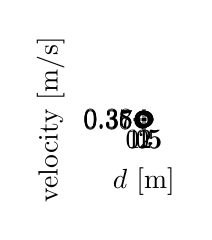
\begin{tikzpicture}

\begin{axis}[%
width=0.951\widthsette,
height=0.75\widthsette,
at={(0\widthsette,0\widthsette)},
scale only axis,
xmin=0,
xmax=2,
xlabel={$d$ [m]},
ymin=0.35,
ymax=0.38,
ylabel={velocity [m/s]},
axis background/.style={fill=white},
xmajorgrids,
ymajorgrids,
yticklabel style={/pgf/number format/.cd,fixed,precision=3}
]
\addplot [color=black, line width=1.0pt, mark size=2.5pt, mark=o, mark options={solid, black}, forget plot]
  table[row sep=crcr]{%
0.05	0.352715\\
0.2	0.371891\\
0.3	0.375066\\
0.5	0.376806\\
1	0.375925\\
1.5	0.374456\\
2	0.373188\\
};
\end{axis}
\end{tikzpicture}%
	\caption[Relation between the maximum velocity above the second cavity and 
	the distance between the cavities]{Relation between the maximum velocity in the peak above the second cavity and the distance $d$ between the cavities.}
	\label{fig:velpeaks}
\end{figure}
We see that if $d < d_{rec}$ the velocity is affected by the presence of 
the first cavity and so its value is lower. For $d>d_{rec}$ the velocity is 
slightly decreasing as $d$ increases; this fact is due to the turbulence that 
is generated near the end of the first cavity. As it can be seen in 
Figure~\ref{fig:kd1}, the turbulent kinetic energy that is generated from the 
first cavity is transported towards the second one, leading to an increased 
thickness of the boundary layer as we move in the $x$-direction.
\begin{figure}
	\centering
	\includegraphics[width=\textwidth,% trim={0 0 0 7cm}, clip 
	]{cavities_dist1_k_report.png}
	\caption[Turbulen kinetic energy in the cavities problem]{Turbulent kinetic energy [$\si{m^2/s^2}$] around the cavities with $d=\SI{1}{m}$, at $t=T_\text{end}$. $Re=\num{6e5}$.}
	\label{fig:kd1}
\end{figure}
%
\subsection{Coupled problem}
%A more complex result.